%============================================================
%  MÉMOIRE D'INGÉNIEUR EN DATA SCIENCES
%  Université de Maroua — ENSPM
%  Auteur : NDZESSA AVELE BRUNO LANDRY
%============================================================

\documentclass[12pt, a4paper, oneside]{report}

%------------------------------------------------------------
%  ENCODAGE & LANGUE
%------------------------------------------------------------
\usepackage[utf8]{inputenc}
\usepackage[T1]{fontenc}
\usepackage[french]{babel}
\usepackage{csquotes}
\usepackage{booktabs}
\usepackage{siunitx}
\usepackage{float}
\usepackage{caption}
\usepackage[table]{xcolor}
\usepackage{newtxtext}
\usepackage{newtxmath}
%------------------------------------------------------------
%  POLICES & TYPOGRAPHIE
%------------------------------------------------------------
\usepackage{lmodern}
\usepackage{microtype}
\usepackage{setspace}
\onehalfspacing

%------------------------------------------------------------
%  GÉOMÉTRIE DE LA PAGE
%------------------------------------------------------------
\usepackage[
top=2.5cm,
bottom=2.5cm,
left=3cm,
right=2.5cm,
headheight=28pt        % CORRECTION 1 : 15pt → 28pt (évite le warning fancyhdr)
]{geometry}

%------------------------------------------------------------
%  EN-TÊTES & PIEDS DE PAGE
%------------------------------------------------------------
\usepackage{fancyhdr}
\pagestyle{fancy}
\fancyhf{}
\fancyhead[L]{\small\textit{\leftmark}}
%\fancyhead[R]{\small\textit{ENSPM — Maroua}}
\fancyfoot[L]{Rédigé par NDZESSA AVELE Bruno Landry}
\fancyfoot[R]{\thepage}
\renewcommand{\headrulewidth}{0pt}
\renewcommand{\footrulewidth}{0pt}

\fancypagestyle{plain}{
	\fancyhf{}
	\fancyfoot[C]{\thepage}
	\renewcommand{\headrulewidth}{0pt}
}
%------------------------------------------------------------
%  COULEURS — VERSION IMPRESSION NOIR ET BLANC
%------------------------------------------------------------
\usepackage[dvipsnames, table]{xcolor}

% Remplace les couleurs vives par du noir et des gris
\definecolor{primary}{RGB}{0, 0, 0}          % noir pur → titres, cadres
\definecolor{secondary}{RGB}{80, 80, 80}     % gris foncé → sous-titres, filets
\definecolor{accent}{RGB}{50, 50, 50}        % gris très foncé → alertes
\definecolor{lightgray}{RGB}{240, 240, 240}  % gris clair → fonds de boîtes
\definecolor{darkgray}{RGB}{60, 60, 60}      % gris foncé → numéros de lignes
%------------------------------------------------------------
%  GRAPHIQUES & FIGURES
%------------------------------------------------------------
\usepackage{graphicx}
\usepackage{float}
\usepackage{subcaption}
\usepackage{wrapfig}
\usepackage{tikz}
\usetikzlibrary{shapes, arrows.meta, positioning, calc, decorations.pathmorphing}

%------------------------------------------------------------
%  TABLEAUX
%------------------------------------------------------------
\usepackage{booktabs}
\usepackage{tabularx}
\usepackage{multirow}
\usepackage{longtable}
\usepackage{array}

%------------------------------------------------------------
%  MATHÉMATIQUES & CODE
%------------------------------------------------------------
%\usepackage{amsmath, amssymb, amsthm}
\usepackage{listings}
\usepackage{algorithm}
\usepackage{algpseudocode}

\lstset{
	basicstyle=\small\ttfamily,
	backgroundcolor=\color{lightgray},
	frame=single,
	framerule=0.5pt,
	rulecolor=\color{secondary},
	breaklines=true,
	numbers=left,
	numberstyle=\tiny\color{darkgray},
	keywordstyle=\color{primary}\bfseries,
	commentstyle=\color{darkgray}\itshape,
	stringstyle=\color{accent},
	captionpos=b,
	xleftmargin=2em,
	xrightmargin=0.5em,
	extendedchars=true,           % CORRECTION 2 : autorise les accents dans lstlisting
	inputencoding=utf8,
	literate=
	{é}{{\'e}}1 {è}{{\`e}}1 {ê}{{\^e}}1 {ë}{{\"e}}1
	{à}{{\`a}}1 {â}{{\^a}}1 {ä}{{\"a}}1
	{ù}{{\`u}}1 {û}{{\^u}}1 {ü}{{\"u}}1
	{î}{{\^i}}1 {ï}{{\"i}}1
	{ô}{{\^o}}1 {ö}{{\"o}}1
	{ç}{{\c{c}}}1 {œ}{{\oe}}1 {æ}{{\ae}}1
	{É}{{\'E}}1 {È}{{\`E}}1 {Ê}{{\^E}}1
	{À}{{\`A}}1 {Â}{{\^A}}1
	{Ç}{{\c{C}}}1,
}

%------------------------------------------------------------
%  HYPERLIENS & PDF METADATA
%  IMPORTANT : hyperref doit toujours être chargé AVANT biblatex
%------------------------------------------------------------
\usepackage[
colorlinks=true,
linkcolor=black,       % ← était primary (bleu)
citecolor=black,       % ← était secondary (bleu clair)
urlcolor=black,        % ← était secondary
bookmarks=true,
pdfauthor={NDZESSA AVELE BRUNO LANDRY},
pdftitle={Plateforme gouvernementale pour la cartographie et mise en relation
	des besoins des entreprises locales},
pdfsubject={Mémoire de fin d'études — Ingénieur en Data Sciences},
pdfkeywords={Data Sciences, Cartographie, Entreprises, MINEPAT, Cameroun}
]{hyperref}
%------------------------------------------------------------
%  BIBLIOGRAPHIE
%  CORRECTION 3 : style=apa nécessite le package biblatex-apa
%  installé via MiKTeX Package Manager
%------------------------------------------------------------
%\usepackage[backend=biber,natbib=true, style=ieee, citestyle=ieee]{biblatex}
 % Ton fichier de références
\usepackage[numbers]{natbib}
%\addbibresource{references.bib}
%\bibliographystyle{plainnat}
%------------------------------------------------------------
%  PERSONNALISATION DES CHAPITRES
%------------------------------------------------------------
\usepackage{titlesec}

\titleformat{\chapter}[display]
{\normalfont\bfseries\color{black}}        % ← était color{primary}
{%
	\hfill
	\tikz[remember picture]{
		\node[fill=black, text=white,           % ← fill était primary
		font=\Large\bfseries,
		minimum width=1.5cm, minimum height=1.5cm,
		rounded corners=4pt]
		{\thechapter};
	}
}
{0pt}
{\vspace{1ex}\huge\raggedright}
[\vspace{0.5ex}{\color{black}\rule{\linewidth}{2pt}}]  % ← était primary

\titleformat{\section}
{\normalfont\large\bfseries\color{black}}  % ← était primary
{\thesection}{1em}{}
[\vspace{-0.5ex}{\color{darkgray}\rule{\linewidth}{0.6pt}}]  % ← était secondary

\titleformat{\subsection}
{\normalfont\normalsize\bfseries\color{black}}   % ← était secondary
{\thesubsection}{1em}{}

\titleformat{\subsubsection}
{\normalfont\normalsize\itshape\color{darkgray}} % ← était darkgray, ok
{\thesubsubsection}{1em}{}

%------------------------------------------------------------
%  TABLE DES MATIÈRES
%------------------------------------------------------------
\usepackage{titletoc}
\usepackage[titles]{tocloft}
\renewcommand{\cftchapfont}{\bfseries\color{black}}
\renewcommand{\cftchappagefont}{\bfseries\color{black}}
\renewcommand{\cftsecfont}{\color{darkgray}}
\setlength{\cftbeforechapskip}{6pt}

%------------------------------------------------------------
%  BOÎTES & ENVIRONNEMENTS SPÉCIAUX
%------------------------------------------------------------
\usepackage{tcolorbox}
\tcbuselibrary{most}

\newtcolorbox{definition}[1][]{
	colback=lightgray, colframe=black,
	title=Définition #1,
	fonttitle=\bfseries,
	arc=4pt, boxrule=0.8pt
}

\newtcolorbox{remarque}{
	colback=blue!5, colframe=darkgray,
	title=Remarque,
	fonttitle=\bfseries\small,
	arc=4pt, boxrule=0.6pt, left=4pt, right=4pt
}

\newtcolorbox{important}{
	colback=red!5, colframe=black,
	title=Important,
	fonttitle=\bfseries\small,
	arc=4pt, boxrule=0.6pt
}

%------------------------------------------------------------
%  LÉGENDES
%------------------------------------------------------------
\usepackage[
labelfont={bf, color=black},
font=small,
justification=centering
]{caption}

%------------------------------------------------------------
%  GLOSSAIRE & ACRONYMES
%  CORRECTION 4 : glossaries chargé APRÈS hyperref (ordre obligatoire)
%------------------------------------------------------------
\usepackage[acronym, nonumberlist]{glossaries}

\makeglossaries

\newacronym{dape}{DAPE}{Division des Analyses et des Politiques Économiques}
\newacronym{minepat}{MINEPAT}{Ministère de l'Économie, de la Planification
	et de l'Aménagement du Territoire}
\newacronym{owasp}{OWASP}{Open Web Application Security Project}
\newacronym{snd30}{SND30}{Stratégie Nationale de Développement  2020-2030}
\newacronym{dgepip}{DGEPIP}{Direction Générale de l'Économie et de la
	Programmation des Investissements Publics}
\newacronym{dgpat}{DGPAT}{Direction Générale de la Planification et de
	l'Aménagement du Territoire}
\newacronym{dgcoop}{DGCOOP}{Direction Générale de la Coopération et de
	l'Intégration Régionale}
\newacronym{dag}{DAG}{Direction des Affaires Générales}
\newacronym{uml}{UML}{Unified Modeling Language}
\newacronym{orm}{ORM}{Object Relational Mapping}
\newacronym{acm}{ACM}{Analyse des Correspondances Multiples}
\newacronym{cah}{CAH}{Classification Ascendante Hièrarchique}
\newacronym{afd}{AFD}{Analyse Factorielle Discriminante}
\newacronym{ins}{INS}{Institut National de la Statistique}
\newacronym{rge}{RGE}{Recensement Général des Entreprises}
\newacronym{cas}{CAS}{Cellule des Analyses Sectorielles}
\newacronym{gecam}{GECAM}{Groupement des Entreprises du Cameroun}
\newacronym{pme}{PME}{Petites et Moyennes Entreprises}
\newacronym{api}{API}{Application Programming Interface}
\newacronym{ml}{ML}{Machine Learning}
\newacronym{sgbd}{SGBD}{Système de Gestion de Bases de Données}
\newacronym{uis}{UI/UX}{User Interface / User Experience}

%------------------------------------------------------------
%  COMMANDES UTILITAIRES
%------------------------------------------------------------
\newcommand{\HRule}{\rule{\linewidth}{0.5mm}}
\newcommand{\auteur}{NDZESSA AVELE Bruno Landry}
\newcommand{\matricule}{21D0180EP}
\newcommand{\directeur}{Pr }
\newcommand{\annee}{2025 / 2026}
\newcommand{\titredoc}{Cartographie des besoins des entreprises camerounaises par analyse multidimensionnelle et développement d'une plateforme gouvernementale de mise en relation}
%============================================================
%  DOCUMENT
%============================================================
\begin{document}
	%------------------------------------------------------------
	%  PAGE DE GARDE
	%------------------------------------------------------------
	\begin{titlepage}
		\newgeometry{top=1.5cm, bottom=1.5cm, left=2.5cm, right=2.5cm}
		\begin{center}
			
			%--- BLOC 1 : En-tête bilingue avec logo université centré ---
			\begin{tabularx}{\textwidth}{>{\centering\arraybackslash}p{4.5cm}
					>{\centering\arraybackslash}X
					>{\centering\arraybackslash}p{4.5cm}}
				\multirow{2}{*}{%
					\parbox[c]{4.2cm}{\centering\small
						République du Cameroun\\[-2pt]
						{\tiny **********}\\[-2pt]
						Paix-Travail-Patrie\\[-2pt]
						{\tiny **********}\\[-2pt]
						Université de Maroua\\[-2pt]
						{\tiny **********}\\[-2pt]
						École Nationale Supérieure\\[-2pt]
						Polytechnique de Maroua}%
				}
				&
				\multirow{2}{*}{%
					\parbox[c]{3cm}{\centering%
						
\includegraphics[height=2.5cm]{LogoUMA.png}}%
				}
				&
				\multirow{2}{*}{%
					\parbox[c]{4.2cm}{\centering\small
						Republic of Cameroon\\[-2pt]
						{\tiny **********}\\[-2pt]
						Peace-Work-Fatherland\\[-2pt]
						{\tiny **********}\\[-2pt]
						The University of Maroua\\[-2pt]
						{\tiny **********}\\[-2pt]
						National Advanced School of\\[-2pt]
						Engineering of Maroua}%
				}
				\\[3.8cm] & & \\
			\end{tabularx}
			
			\vspace{0.3cm}
			\textcolor{primary}{\rule{\linewidth}{1.5pt}}
			\vspace{0.15cm}
			
			%--- BLOC 2 : Bandeau département avec logos ENSPM et MINEPAT ---
			\begin{tabularx}{\textwidth}{>{\centering\arraybackslash}p{3cm}
					>{\centering\arraybackslash}X
					>{\centering\arraybackslash}p{3cm}}
				\multirow{2}{*}{%
					\raisebox{-1\totalheight}{%
						
\includegraphics[height=1.8cm]{LogoENSPM.jpeg}%
					}%
				}
				&
				\multirow{2}{*}{%
					\parbox[c]{7cm}{\centering
						\textbf{\large\color{primary} DÉPARTEMENT D'INFORMATIQUE}\\[2pt]
						\textbf{\large\color{primary} ET TÉLÉCOMMUNICATIONS}}%
				}
				&
				\multirow{2}{*}{%
					\raisebox{-1\totalheight}{%
						
\includegraphics[height=1.8cm]{minepat.png}%
					}%
				}
				\\[1.4cm] & & \\
			\end{tabularx}
			
			\vspace{0.15cm}
			\textcolor{primary}{\rule{\linewidth}{1.5pt}}
			\vspace{0.5cm}
			
			%--- BLOC 3 : Titre du mémoire ---
			\begin{tcolorbox}[
				colback=primary!6, colframe=primary,
				arc=5pt, boxrule=1pt,
				left=12pt, right=12pt, top=10pt, bottom=10pt
				]
				\centering
				{\large\bfseries\color{primary} \titredoc}
			\end{tcolorbox}
			
			\vspace{0.45cm}
			
			%--- BLOC 4 : Nature du document ---
			{\normalsize Mémoire présenté et soutenu en vue de l'obtention du}\\[5pt]
			{\large\bfseries\color{primary} Diplôme d'Ingénieur  en Data Sciences}
			
			\vspace{0.45cm}
			
			%--- BLOC 5 : Auteur ---
			{\normalsize Par }\\[5pt]
			{\large\bfseries \auteur}\\[3pt]
			{\small Matricule : \matricule}
			
			\vspace{0.4cm}
			
			%--- BLOC 6 : Encadrement ---
			{\normalsize Sous la direction de :}\\[5pt]
			{\large\bfseries\color{primary} Pr KALADZAVI Guidedi}\\[2pt]
			{\small Ma\^itre de conférences}
			
			\vspace{0.4cm}
			
			%--- BLOC 7 : Jury ---
			\begin{tabularx}{\textwidth}{>{\bfseries\raggedright\arraybackslash}p{3.2cm}
					>{\raggedright\arraybackslash}X}
				\multicolumn{2}{c}{\normalsize\bfseries Devant le jury composé de :}\\[6pt]
				Président :    & Pr MOULLA KOULLA Donatien \\[4pt]
				Rapporteur :   & Pr KALADZAVI Guidedi \\[4pt]
				Examinatrice : & Dr BOUDJOU Hortense \\[4pt]
				Invité: & M. Abdelaziz Junmbe
			\end{tabularx}
			
			\vfill
			
			%--- BLOC 8 : Pied de page ---
			\textcolor{primary}{\rule{\linewidth}{1pt}}\\[5pt]
			{\bfseries Année Académique \annee}
			
		\end{center}
		\restoregeometry
	\end{titlepage}
	
	%------------------------------------------------------------
	%  PAGES LIMINAIRES (numérotation romaine)
	%------------------------------------------------------------
%	\frontmatter   % Si vous utilisez \mainmatter plus loin
	% Sinon, utilisez : \pagenumbering{roman}
	\pagenumbering{roman}
	\setcounter{page}{1}
	
	%--- DÉDICACE ---
	\chapter*{Dédicace}
	\addcontentsline{toc}{chapter}{Dédicace}
	\thispagestyle{plain}
	
	\vspace{4cm}
	\begin{flushright}
		\begin{minipage}{0.6\textwidth}
			\itshape\large
			Je dédie ce travail à ma famille.
		\end{minipage}
	\end{flushright}
	\vfill
	
	%--- REMERCIEMENTS ---
	\chapter*{Remerciements}
	\addcontentsline{toc}{chapter}{Remerciements}
	\thispagestyle{plain}
	Ce travail n'aurait pas vu le jour sans l'apport considérable de 
	 nombreuses personnes. Nous remercions sincèrement :
	
	\begin{itemize}
		\item \textbf{Pr MOULLA KOULLA Donatien}, pour l'honneur qu'il nous fait de présider le jury de cette soutenance;
		\item \textbf{Dr BOUDJOU Hortense}, pour avoir accepter d'examiner ce travail et pour les observations, remarques et suggestions dans le seul but d'améliorer ce travail; 
		\item \textbf{Pr KALADZAVI Guidedi}  Chef du Département d'Informatique et Télécommunications et notre encadreur académique pour les réformes et améliorations apporté à ce travail;
		\item Tous les \textbf{enseignants} qui, à travers leurs enseignements, ont rendu ce travail possible;
		\item \textbf{M. ALAMINE OUSMANE MEY} Ministre de l'Economie de la Planification et de l'Aménagement du Territoire pour nous avoir accordé la possibilité d'effectuer un stage académique au sein de la structure dont il a la charge;
		\item \textbf{M. MENDO PAULIN} chef de la \gls{dape} pour l'accueil chaleureux et l'accompagnement permanent dont nous avons fait l'objet;
		\item \textbf{M. ABDELAZIZ JUNMBE} Cadre à la \gls{cas} et notre encadreur professionnel pour ses conseils avisés et le suivi à la loupe de l'évolution de ce travail;
		\item  \textbf{Notre grande famille} pour les sacrifices consentis;
		\item \textbf{Nos camarades} pour le soutien et la solidarité dont ils ont fait preuve;
		\item Tous ceux qui de près ou de loin ont contribué à l'aboutissement de ce travail.
	\end{itemize}
	
	%--- TABLE DES MATIERES ---
	\tableofcontents
	\addcontentsline{toc}{chapter}{Table des matières}
	
%--- LISTE DES ACRONYMES ---
\printglossary[type=\acronymtype, title={Liste des abréviations}]
\addcontentsline{toc}{chapter}{Liste des acronymes et abréviations}

	%--- RÉSUMÉ ---
\chapter*{Résumé}
\addcontentsline{toc}{chapter}{Résumé}
\thispagestyle{plain}
Le secteur économique privé camerounais fait face à des difficultés manifestes qui entravent sa croissance et sa pérennité. Afin de dynamiser ce tissu économique, le présent travail s'articule autour d'un double objectif : analyser les données d'une enquête nationale initiée par le \gls{minepat} pour cartographier précisément les besoins des entreprises, puis concevoir une plateforme numérique de mise en relation des entreprises. Les variables issues de la dite enqu\^ete étant essentiellement catégorielles, une démarche d'analyse factorielle combinant statistiques descriptives (uni-variées et bis-variées) et classification automatique a été déployée. L'analyse révèle que $96{,}23\,\%$ des structures recensées présentent un besoin de financement, le secteur d'activité s'imposant comme la variable qui permet le mieux de segmenter la nature des besoins. De plus, une forte dépendance est mise en évidence entre l'ancienneté des entreprises et leurs exigences en matière de recherche et d'innovation. L'application de la Classification Ascendante Hiérarchique (CAH) a permis de partitionner le secteur privé en trois profils distincts. La première catégorie, qualifiée d'acteurs agro-productifs émergents, regroupe les petites structures évoluant majoritairement dans l'agroalimentaire ($81{,}1\,\%$) et ayant une ancienneté de 5 à 9 ans. La deuxième catégorie, identifiée comme les opérateurs financiers et autres services établis, représente des entreprises plus matures, dont $26{,}6\,\%$ affichent plus de 20 ans d'existence, orientées principalement vers les services financiers et bancaires. Enfin, la troisième catégorie, nommée les petites entreprises multiple-sectorielles, est constituée de jeunes structures en phase de démarrage opérant à $68{,}8\,\%$ dans des secteurs diversifiés hors agroalimentaire. Le second volet de ce travail est consacré au développement de la plateforme «~Business Partnership~». Adoptant une approche orientée vers la performance, la base de données sous-jacente a fait l'objet d'une modélisation dimensionnelle, optimisant ainsi la fluidité et l'efficacité des requêtes SQL lors des recherches de partenariats.

\vspace{0.5cm}
\noindent \textbf{Mots-clés :} Plateforme numérique, cartographie des besoins,  secteur privé.
%	[Insérer ici le résumé en français — environ 200 à 300 mots décrivant le contexte, les objectifs, la méthodologie et les résultats principaux de votre travail.]
	
	\vspace{1cm}

	\chapter*{Abstract}
	\addcontentsline{toc}{chapter}{Abstract}
	\thispagestyle{plain}
	The Cameroonian private sector faces clear difficulties that hinder its growth and sustainability. In order to revitalize this economic fabric, this work revolves around a dual objective: analyzing data from a national survey initiated by the \gls{minepat} to precisely map business needs, and then designing a digital matchmaking platform for enterprises. Since the variables from this survey are essentially categorical, a factor analysis approach combining descriptive statistics (univariate and bivariate) and automatic classification was deployed. The analysis reveals that $96.23\,\%$ of the surveyed entities suffer from a critical funding deficit, with the sector of activity emerging as the variable that best segments the nature of these needs. Furthermore, a strong dependence is highlighted between the seniority of the companies and their requirements in terms of research and innovation. The application of Hierarchical Cluster Analysis (HCA) made it possible to partition the entrepreneurial fabric into three distinct profiles. The first category, described as emerging agro-productive actors, brings together small entities operating mainly in the agri-food sector ($81.1\,\%$) and having 5 to 9 years of seniority. The second category, identified as established financial operators and other services, represents more mature companies, $26.6\,\%$ of which have been in existence for more than 20 years, primarily focused on financial and banking services. Finally, the third category, named small multisectoral enterprises, consists of young startup entities with $68.8\,\%$ operating in diversified sectors outside of agri-food. The second part of this work is dedicated to the development of the "Business Partnership" platform. Adopting a performance-oriented approach, the underlying database underwent dimensional modeling, thereby optimizing the fluidity and efficiency of SQL queries during partnership searches.\vspace{0.5cm}
	
	 \textbf{Keywords:} Digital platform, needs mapping, private sector.
%	\textbf{Keywords:} Digital platform, business mapping, matching system, Data Sciences, MINEPAT, private sector, Cameroon.
	
	\medskip
	
%	[Insert here the English abstract — approximately 200 to 300 words describing the context, objectives, methodology and main results of your work.]
	

	%--- LISTE DES TABLEAUX ---
\listoftables
\addcontentsline{toc}{chapter}{Liste des tableaux}


	%--- LISTE DES FIGURES ---
	\listoffigures
	\addcontentsline{toc}{chapter}{Liste des figures}
	

	
	
	%============================================================
	%  CORPS DU MÉMOIRE (numérotation arabe)
	%============================================================
	\pagenumbering{arabic}
	\setcounter{page}{1}
	
	%------------------------------------------------------------
	%  INTRODUCTION GÉNÉRALE
	%------------------------------------------------------------
	\chapter*{Introduction Générale}
	\addcontentsline{toc}{chapter}{Introduction Générale}
	\markboth{Introduction Générale}{Introduction Générale}
	
La capacité à collaborer et à tisser des relations inter-entreprises pourrait contribuer à la croissance, la compétitivité et la pérennité des entreprises du secteur privé. Au Cameroun, ce besoin de collaboration est d'une grande importance du fait des ambitions portées par la \gls{snd30}, qui place le développement du secteur privé au cœur de l'émergence nationale\cite{minepat2020}.

 
Nous pouvons tout de m\^eme relever que, malgré la présence de divers dispositifs de mise en relation à l'instar des plateformes numériques B2B(LinkedIn, Facebook Marketplace, Alibaba), de la Bourse de Sous-Traitance et de Partenariat (BSTP) ou des dynamiques contractuelles directes les performances globales du secteur privé demeurent en deçà des attentes au vue des résultats de l'évaluation mi-parcours de la \gls{snd30} \cite{minepat2025}. Ce constat met en lumière une inadéquation potentielle entre les outils de collaboration actuelles et les réalités auxquelles font face les entreprises du secteur privé camerounais. En effet, aucun dispositif institutionnel ne permet aujourd'hui aux entreprises d'identifier précisément leurs besoins spécifiques et de bénéficier d'un réseau d'entreprises susceptibles de les accompagner dans leurs différentes activités. 

Dès lors, se pose le problème de la capacité à recenser les besoins des entreprises, à construire des profils d'entreprises sur la base de ces besoins et à concevoir une plateforme numérique de mise en relation sur la base des services offerts et des besoins exprimés. Face à ce défi, notre réflexion est guidée par les préoccupations centrales suivantes : Comment identifier des profils de besoins homogènes d'entreprises à partir des données de l'enqu\^ete réalisée par le MINEPAT? Comment exploiter ces profils ? Et enfin comment concevoir et implémenter une plateforme de mise en relation sur la base des besoins et offres exprimés?

Pour répondre à cela, notre travail s'articule autour de cinq chapitres :

Le chapitre 1 présente la structure d'accueil, expose le contexte global de l'étude et formalise la problématique identifiée sur le terrain. Le chapitre 2 est dédié au cadre théorique et à l'état de l'art. Il s'attèle à définir les concepts clés liés à la collaboration inter-entreprises et analyse de manière critique les solutions existantes afin d'en ressortir les limites techniques et fonctionnelles. Les chapitres 3 et 4 constituent le cœur méthodologique de notre travail, détaillant successivement la phase de conception et la phase de réalisation, où les choix technologiques et les modélisations sont explicités. Le chapitre 5 évalue et présente les résultats obtenus, validant la pertinence fonctionnelle de la solution développée. Enfin, une conclusion générale viendra dresser le bilan de nos travaux et ouvrir des perspectives d'amélioration pour les développements futurs.

	%============================================================
	%  CHAPITRE 1 : PRÉSENTATION DE LA STRUCTURE ET DU STAGE
	%============================================================
	\chapter{Présentation du cadre de l'étude}
	\label{chap:structure}
Ce chapitre pr\'esente le cadre institutionnel et probl\'ematique
dans lequel s'inscrit ce travail. Il est organis\'e en deux parties.
La premi\`ere d\'ecrit l'organisation et les missions du \gls{minepat},
structure au sein de laquelle le stage acad\'emique a \'et\'e
effectu\'e. La seconde expose le contexte \'economique national,
identifie les lacunes des initiatives existantes en mati\`ere de
connaissance des besoins des entreprises, et formule la
probl\'ematique ainsi que la d\'emarche m\'ethodologique retenue.
\section[Présentation du MINEPAT]{Présentation du \gls{minepat}}
\label{sec:minepat}

Le Ministère de l'Économie, de la Planification et de l'Aménagement du Territoire
(\gls{minepat}), créé par le Décret N°\,2008/220 du 4 juillet 2008, est l'institution
gouvernementale chargée de l'élaboration et de la mise en \oe uvre de la politique
économique nationale ainsi que de l'aménagement du territoire \cite{decret2008}. Placé sous l'autorité
d'un Ministre assisté d'un Ministre délégué, le \gls{minepat} s'appuie sur un ensemble
de structures organisationnelles complémentaires pour accomplir ses missions, le ministre est accompagné par: un
Secrétaire particulier, quatre conseillers techniques, une Inspection Générale, une
administration centrale, des services déconcentrés, des services extérieurs ainsi que
des établissements et organismes rattachés. Le ministre délégué dispose d'un secrétaire particulier.

%------------------------------------------------------------
\subsection{Organisation interne du \gls{minepat}}
%------------------------------------------------------------

\subsubsection{Le Ministre délégué}

Le Ministre délégué est chargé d'assister le Ministre dans l'exercice de ses fonctions.
Il dispose à cet effet d'un Secrétariat particulier et peut se voir déléguer des
attributions spécifiques par le Ministre.

\subsubsection{L'Inspection Générale}

L'Inspection Générale est placée sous l'autorité d'un Inspecteur Général dont la
mission principale est l'évaluation des performances des services du Ministère. Elle
veille à la bonne application des directives ministérielles, contrôle la régularité des
opérations administratives et financières, et formule des recommandations en vue de
l'amélioration du fonctionnement interne des structures.

\subsubsection{L'Administration Centrale}

L'administration centrale constitue le c\oe ur opérationnel du \gls{minepat}. Elle est
composée des structures suivantes~:

\begin{enumerate}
	
	\item \textbf{Le Secrétariat Général (SG)}~: il assure la coordination administrative
	de l'ensemble des directions et divisions du Ministère. Il comprend notamment la
	Division des Affaires Juridiques, la Division de la Promotion des Relations Publiques
	et de la Communication, la Division Informatique, la Division de Suivi et de la
	Relance, la Cellule de Traduction, la Sous-Direction de l'Accueil du Courrier et de
	Liaison, ainsi que la Sous-Direction de la Documentation et des Archives.
	
	\item \textbf{La Direction Générale de l'Économie et de la Programmation des
		Investissements Publics (DGEPIP)}~: elle est chargée du suivi de la conjoncture
	économique, de la programmation des investissements publics et de l'élaboration des
	cadres de dépenses à moyen terme. Elle comprend la Division des Analyses et des
	Politiques Économiques (DAPE) --- au sein de laquelle s'est déroulé le présent
	stage ---, la Division de la Prévision et de la Préparation des Programmes et
	Projets, ainsi que la Direction de la Programmation des Investissements Publics.
	
	\item \textbf{La Direction Générale de la Planification et de l'Aménagement du
		Territoire (DGPAT)}~: elle est responsable des études prospectives, de la planification
	stratégique et de l'aménagement du territoire. Elle regroupe la Division de la
	Prospective et de la Planification Stratégique, la Division des Analyses
	Démographiques et des Migrations, la Direction de l'Aménagement du Territoire et
	de la mise en valeur des Zones Frontalières, ainsi que la Direction des
	Infrastructures et d'Appui au Développement Régional et Local.
	
	\item \textbf{La Direction Générale de la Coopération et de l'Intégration Régionale
		(DGCOOP)}~: elle gère les relations de coopération bilatérale et multilatérale du
	Cameroun. Elle comprend la Direction de la Coopération Nord-Sud et des
	Organisations multilatérales, la Direction de l'Intégration Régionale, la Division
	de la Coopération avec les Pays Émergents, la Division de la Coopération avec le
	Monde Islamique, le Service du Fichier des Accords et des Conventions, ainsi que
	le Service d'Appui à la Coopération Décentralisée.
	
	\item \textbf{La Direction des Affaires Générales (DAG)}~: elle assure la gestion
	des ressources humaines, budgétaires et matérielles du Ministère. Elle comprend la
	Sous-Direction des Personnels, de la Solde et des Pensions, la Sous-Direction du
	Budget, la Sous-Direction des Ressources Humaines, la Sous-Direction de
	l'Équipement et de la Maintenance, ainsi que la Cellule SIGIPES (Système
	Informatique de Gestion Intégré des Personnels de l'État et de la Solde).
	
\end{enumerate}

\subsubsection{Les Services Déconcentrés}

Les services déconcentrés assurent la représentation du \gls{minepat} à l'échelle
territoriale. Ils sont composés des Délégations Régionales de l'Économie, de la
Planification et de l'Aménagement du Territoire, présentes dans chacune des dix
régions du Cameroun, ainsi que des Délégations Départementales de l'Économie, de
la Planification et de l'Aménagement du Territoire, dont le rôle est d'assurer le
relais des politiques nationales au niveau des départements.

\subsubsection{Les Établissements et Organismes Rattachés}

Le \gls{minepat} supervise plusieurs établissements spécialisés qui contribuent à la
production de données statistiques et à la mise en \oe uvre des politiques publiques.
Il s'agit notamment~:

\begin{itemize}
	\item des Missions d'Aménagement du Territoire~: MIDIMA, MEADEN et MEAO~;
	\item du Bureau Central des Recensements et des Études de Population
	\textbf{(BUCREP)}~;
	\item de l'Institut National de la Statistique \textbf{(INS)}, principal producteur
	de données statistiques officielles au Cameroun~;
	\item de l'Institut Panafricain pour le Développement \textbf{(IPD)}~;
	\item de l'Institut Sous-régional de Statistique et d'Économie Appliquée
	\textbf{(ISSEA)}~;
	\item de l'Institut de Formation et de Recherche Démographique \textbf{(IFORD)}~;
	\item du Comité Technique de Préparation et de Suivi du Programme d'Ajustement
	Structurel \textbf{(CTS)}.
\end{itemize}

%------------------------------------------------------------
\subsection[Missions du MINEPAT]{Missions du \gls{minepat}}
%------------------------------------------------------------

Le \gls{minepat} est en charge de l'élaboration et de la mise en \oe uvre de la
politique économique de la Nation ainsi que de l'aménagement du territoire. Ses
missions s'articulent autour de trois axes principaux.

\subsubsection{En matière d'économie}

Dans le domaine économique, le \gls{minepat} est chargé~:
\begin{enumerate}
	\item de la cohérence et de la coordination des actions engagées avec les partenaires
	internationaux et bilatéraux dans le cadre du programme de redressement et de
	relance économiques~;
	\item du suivi de la coopération sous-régionale et internationale, notamment avecùle
	Programme des Nations Unies pour le Développement (PNUD), la Commission
	Économique des Nations Unies pour l'Afrique (CEA), la Communauté Économique
	et Monétaire de l'Afrique Centrale (CEMAC) et la Communauté Économique des
	États de l'Afrique Centrale (CEEAC)~;
	\item de la prospection, de la négociation, de la finalisation et du suivi de
	l'exécution des accords et conventions de prêts, ainsi que de la gestion de
	la banque de projets et de la promotion des investissements publics~;
	\item de la préparation des cadres de dépenses à moyen terme et du budget
	d'investissement public~;
	\item du suivi et du contrôle des programmes et projets d'investissement, en liaison
	avec les ministères sectoriels et le ministère chargé des finances.
\end{enumerate}

\subsubsection{En matière de planification}

Dans le domaine de la planification, le \gls{minepat} est chargé~:
\begin{enumerate}
	\item de la réalisation des études et des analyses prospectives sur le développement
	du pays à moyen et long terme~;
	\item de l'élaboration d'un cadre global de planification stratégique et de la
	cohérence des stratégies sectorielles de développement~;
	\item de la coordination et du suivi de la mise en \oe uvre de la stratégie de
	réduction de la pauvreté~;
	\item du suivi de la coordination de la politique de développement économique et
	social du Gouvernement.
\end{enumerate}

\subsubsection{En matière d'aménagement du territoire}

Dans le domaine de l'aménagement du territoire, le \gls{minepat} est chargé~:
\begin{enumerate}
	\item de la coordination et de la réalisation des études d'aménagement du territoire,
	tant au niveau national que régional~;
	\item de l'élaboration des normes et règles d'aménagement du territoire et du
	contrôle de leur application~;
	\item du suivi et du contrôle de la mise en \oe uvre des programmes nationaux,
	régionaux ou locaux d'aménagement du territoire~;
	\item du suivi des organisations sous-régionales chargées de l'aménagement ou de
	la préservation de l'écosystème sous-régional.
\end{enumerate}

%------------------------------------------------------------
\subsection{Présentation de la structure d'accueil : la \gls{dape}}
%------------------------------------------------------------

Au sein de la \gls{dgepip}, la Division des Analyses et des Politiques Économiques (\gls{dape})
constitue la structure au sein de laquelle s'est déroulé le présent stage. La \gls{dape} est
organisée en quatre cellules spécialisées dont les missions couvrent l'ensemble du
cycle d'analyse économique~:

\begin{itemize}
	\item \textbf{La Cellule des Analyses Conjoncturelles}~: elle assure le suivi de
	l'évolution à court terme de l'économie camerounaise et produit des notes
	périodiques sur la conjoncture nationale et internationale~;
	\item \textbf{La Cellule des Politiques Économiques}~: elle évalue la cohérence et
	l'impact des politiques économiques mises en \oe uvre par le Gouvernement~;
	\item \textbf{La Cellule de Synthèse Macroéconomique}~: elle produit des analyses
	consolidées sur les grands équilibres macroéconomiques, notamment les comptes
	nationaux, la balance des paiements et les finances publiques~;
	\item \textbf{La Cellule des Analyses Sectorielles}~: elle est chargée du suivi des
	performances sectorielles et de l'analyse des contributions des différents
	secteurs à la croissance économique nationale. C'est au sein de cette cellule
	que les missions décrites dans la section suivante ont été accomplies.
\end{itemize}
	\begin{figure}[H]           % H = ici exactement
		\centering
		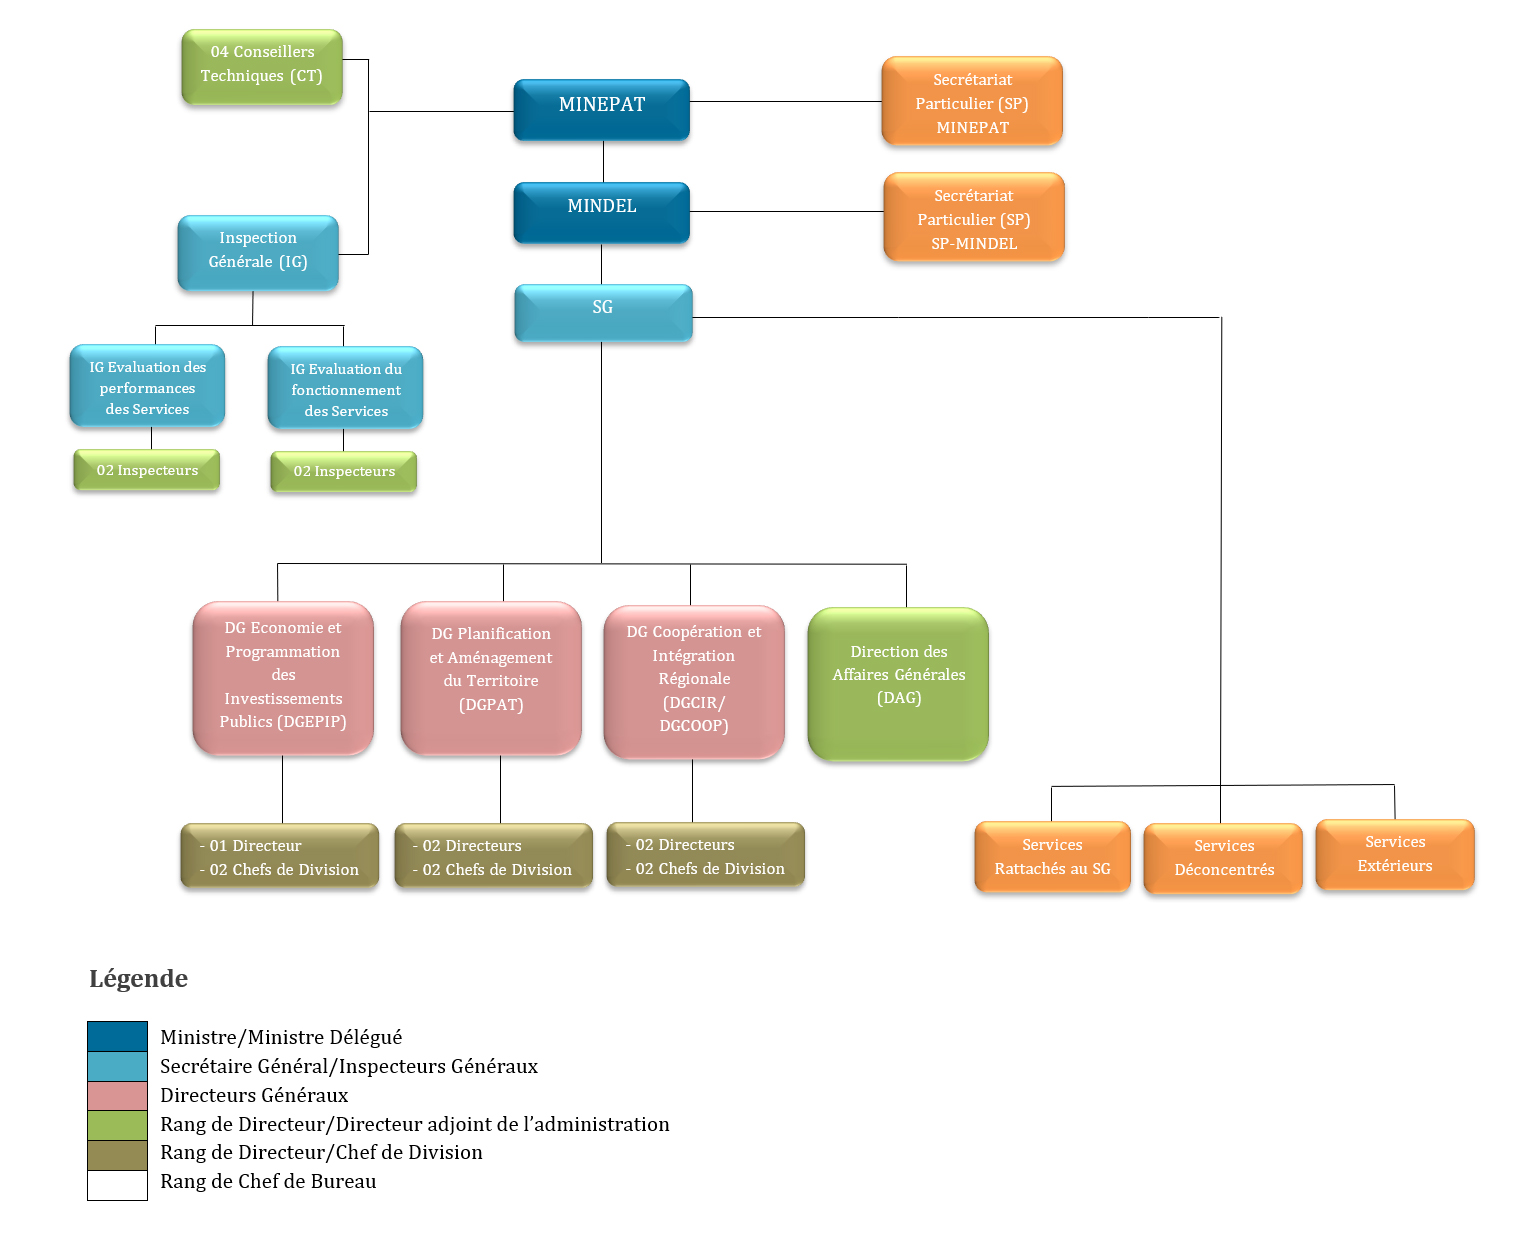
\includegraphics[width=0.8\textwidth]{Organigramme4.jpg}
		\caption[Organigramme simplifié du MINEPAT]{Organigramme simplifié du \gls{minepat} \footnotemark}
		\label{fig:organigramme}
	\end{figure}
	\footnotetext{Source : Site web MINEPAT}
	\section{Contexte et problématique}
	
	\subsection{Contexte}
	Dans de nombreux pays en développement, les entreprises locales jouent un rôle déterminant en ce qui concerne la production de biens et services, la création de valeur ajoutée et la dynamisation de l’activité économique \cite{fmi2023}. C’est la raison pour laquelle depuis 2009, le Cameroun s’est fixé pour objectif : le développement du secteur privé \cite{minepat2009}. En effet, selon la vision à l'horizon 2035 , le développement de ce secteur constitue un levier essentiel de croissance économique, de création d’emplois et de transformation structurelle des économies. 
	Conscient de l’importance de ce secteur dans le développement économique, le Gouvernement camerounais a adopté la Stratégie Nationale de Développement 2020-2030 \cite{minepat2020}, qui constitue le cadre de référence des politiques économiques et sociales pour la période 2020-2030. Cette stratégie vise notamment à accélérer la transformation structurelle de l’économie afin de faire du Cameroun un pays émergent à l’horizon 2035 \cite{minepat2020}.\\ 
	
	Dans ce cadre, plusieurs réformes ont déjà été mis en œuvre afin d’améliorer le climat des affaires et de promouvoir le développement du secteur privé \cite{minepat2025}. Il s’agit notamment de : (i) la révision du cadre légal et réglementaire régissant le régime foncier et domanial en cohérence avec l’industrialisation, la modernisation de l’agriculture, le développement des villes, de l’immobilier et du logement ; (ii) la relecture du cadre légal et réglementaire de la gouvernance et de gestion de la forêt, pêche et élevage en cohérence avec l’industrialisation ; (iii) la relecture du cadre légal et réglementaire de la publicité en lien avec l’économie de marché et de commerce électronique ou en ligne ; (iv) la mise en place d’un cadre légal et réglementaire de structuration du sous-secteur de la médecine traditionnelle en vue de vulgariser les médicaments locaux ; et (v) la création et la mise en place des juridictions spécialisées pour améliorer l’instruction des litiges commerciaux et financiers.\\
	
	Toutefois, malgré la mise en œuvre de ces réformes, les performances économiques observées restent bien loin  des objectifs fixés. Selon le rapport d’évaluation de mi-parcours de la SND30 rendu public par le MINEPAT en janvier 2026, la croissance économique qui devait atteindre environ 8,5 \% en 2025, s’est établie en moyenne à 3,4 \% entre 2020 et 2025, avec des taux annuels de 0,3 \% en 2020, 3,3 \% en 2021, 3,7 \% en 2022, 3,2 \% en 2023 et environ 3,5 \% en 2024. De même, la contribution du secteur industriel à l’économie reste inférieure aux objectifs fixés. En effet, la part de la valeur ajoutée manufacturières sur le PIB stagne à 14 \% entre 2020-2025 au lieu des 19,9 \% prévus. Par ailleurs, le crédit à l’économie plafonne à 17,5 \% contre un objectif de 23,2 \% \cite{minepat2025}. \\
	
	Ces résultats montrent que, malgré les réformes engagées, plusieurs contraintes continuent de limiter le développement des entreprises locales. Pour rattraper les écarts observés, Monsieur le Ministre de l’Economie de la planification et de l’Aménagement du Territoire a instruit à la Division des Analyses et des Politiques Economiques (DAPE) la mise en œuvre d’une étude visant à faire la cartographie des besoins des entreprises du tissu productif local. Les extrants de cette étude permettront au Gouvernement de mener des interventions plus ciblées et adaptées aux entreprises selon leurs besoins.
	
	
	\subsection{Problématique}
	
	Les difficultés et besoins des entreprises ont fait l’objet de plusieurs études. Le \gls{gecam} par le biais d’une enquête montre que près de 60\% d’entreprises font face à des difficultés parmi lesquelles, l’instabilité du système fiscal (72\%), les pénalités et amendes fiscales (66\%), le niveau du taux d’imposition (61\%) ainsi la multiplicité des contrôles de l’administration fiscale (59\%) \cite{gecam2019}. Pour le MINEPAT  l’accès à l’énergie électrique est la principale difficulté auxquelles font face les entreprises industrielles nationales \cite{minepat2022}. Aussi, à travers l’enquête sur le climat des affaires au Cameroun auprès des chefs d’entreprises du secteur industriel, le MINEPAT  soulève deux difficultés majeurs auxquelles sont confrontés les entreprises constituant le tissu productif nationale à savoir : l’accès aux facteurs de production et l’état des infrastructures routières \cite{minepat2023}. \\
	
	Il ressort qu’aucune de ces études n’a tenté de recueillir de manière exhaustive les besoins des entreprises locales qui constituent le tissu productif camerounais. En général, elles recueillent les besoins dans le cadre des enquêtes qui poursuivent d’autres objectifs et de ce fait, ne sont pas exhausif. En effet, l’étude du \gls{gecam} , bien que pertinente, se limite aux seuls membres de ce groupement et ne rend pas compte de la diversité du tissu économique national dans son ensemble. Le \gls{minepat}, pour sa part, demeure centré sur le secteur industriel et n’adresse pas de manière suffisamment directe les besoins des acteurs privés dans leur pluralité.\\
	
	C’est pour combler ces lacunes que le \gls{minepat} a engagé une enquête spécifiquement dédiée à la cartographie des besoins des entreprises du tissu productif local, dont les résultats permettront au Gouvernement de mener des interventions plus ciblées et adaptées aux entreprises selon leurs besoins. Au-delà de ce cela, la mise sur pied d’une plateforme numérique de mise en relation des entreprises par le MINEPAT est considérée comme un prolongement naturel de cette démarche. Car, à ce jour, aucun outil de ce type n’existe dans le paysage institutionnel camerounais.\\
	
	Dès lors, deux questions principales guident ce travail : 
	\begin{itemize}
		\item Quels sont les profils de besoins des entreprises locales au Cameroun ? 
		\item Comment développer et mettre en place une plateforme institutionnelle de mise en relation des entreprises locales dans le but de combler leurs besoins ?
	\end{itemize}
	\newpage
	\subsection{Objectifs du mémoire}
	L’objectif général de ce travail est de proposer une cartographie des besoins des entreprises locales sur la base des données obtenues à la suite de l’enquête initiée par la \gls{dape}, de concevoir et de développer une plateforme gouvernementale numérique permettant d’assurer la mise en relation des entreprises. Spécifiquement, il sera question de :
	\begin{itemize}
		\item Identifier et caractériser les besoins exprimés par les entreprises locales à partir des données de l'enquête ;
		\item Établir une cartographie des besoins en fonction des caractéristiques des entreprises au moyen de méthodes d'analyse de données ;
		\item Concevoir l'architecture fonctionnelle et technique d'une plateforme gouvernementale de mise en relation des entreprises ;
		\item Développer et tester un prototype fonctionnel de cette plateforme afin de vérifier la mise en œuvre des fonctionnalités définies.
	\end{itemize}
	%=============================================================

	%-------------------------------------------------------------
	\subsection{Méthodologie générale}
	\label{sec:methodologie_generale}
	%-------------------------------------------------------------
	
	Afin de répondre aux problématiques centrales de ce travail 
	à savoir l'identification des profils des besoins des entreprises et la conception d'une plateforme gouvernementale permettant
	la mise en relation des entreprises une
	démarche méthodologique structurée en deux axes complémentaires
	a été adoptée. Une approche analytique fondée sur le
	traitement statistique des données de l'enquête du \gls{minepat}
	et une approche technique fondée sur le développement d'une
	application web fonctionnelle.
	\subsubsection{Méthodologie d'analyse des données}
	Le premier axe de la démarche porte sur l'analyse statistique
	des données collectées lors de l'enquête nationale sur la
	cartographie et les besoins des entreprises conduite par le
	\gls{minepat} en 2025. Les données étant essentiellement de
	nature qualitative secteur d'activité, région d'implantation,
	taille, ancienneté, types de besoins exprimés une chaîne
	analytique adaptée à ce type de variables a été retenue,
	combinant des méthodes de description uni-variée et bis-variée et
	des méthodes multidimensionnelles éprouvées dans la littérature
	statistique.
	\begin{itemize}
		\item Dans un premier temps, une analyse uni-variée a
		permis de décrire la distribution des entreprises selon chacune
		de leurs caractéristiques, offrant une première photographie
		descriptive du tissu productif couvert par l'enquête.
		\item Dans un
		second temps, une analyse bis-variée fondée sur le test du
		$\chi^2$ de Pearson et le coefficient $V$ de Cramér a permis
		d'identifier et de quantifier les associations entre les
		caractéristiques des entreprises et leurs besoins exprimés.
		\item Dans un troisième temps,
		une \gls{acm} a été
		conduite afin de réduire la dimension des données et de
		produire une représentation factorielle synthétique du nuage
		d'entreprises dans un espace de dimension réduite. Les
		coordonnées factorielles issues de l'ACM ont ensuite alimenté
		une \gls{cah},
		conduite selon le critère d'agrégation de Ward, permettant de
		regrouper les entreprises en classes homogènes aux profils de
		besoins similaires.
		\item Enfin, une \gls{afd} a été appliquée afin de valider la robustesse de
		la partition obtenue, d'identifier les variables les plus
		discriminantes entre les classes et d'élaborer une règle de
		prédiction de classe pour les nouvelles entreprises s'inscrivant
		sur la plateforme.
	\end{itemize}
	L'ensemble de ces analyses a été conduit sous
	le logiciel \textbf{R}, en mobilisant les packages
	\texttt{FactoMineR}, \texttt{factoextra} et \texttt{caret},
	reconnus comme références dans le domaine de l'analyse
	multidimensionnelle \citep{husson_le_pages_2009}.
	
	\subsubsection{Méthodologie de conception de la plateforme}
	Le second axe de la démarche porte sur la conception et le
	développement de la plateforme numérique gouvernementale
	\textit{Business Partnership}. La conception de la base de données
	a été réalisée selon la méthode \textbf{dimensionnelle} où deux tables de dimensions et une table de fait ont été créé. Nous avons élaborer
	ce schéma de la base de données via l'\gls{orm} de Django, afin de garantir une structure relationnelle
	cohérente, évolutive et adaptée aux exigences fonctionnelles
	de la plateforme. Le développement de
	l'application a été conduit en suivant le paradigme MVT
	(Modèle-Vue-Template) qui assure une séparation nette des
	responsabilités entre la logique de données, la logique métier
	et la couche de présentation.
	
	Le c\oe ur fonctionnel 
	de la plateforme est une requete SQL qui permet de mettre en relation des entreprises ayant des besoins et des offres de services communs. 
	
	  La gestion de projet a été conduite selon la méthode
	agile \textbf{Kanban}, qui a permis de maintenir une organisation
	rigoureuse et transparente tout au long du développement, en
	adaptant continuellement les priorités en fonction de l'évolution
	des contraintes académiques et techniques \citep{anderson_2010}.
	\subsubsection{M\'ethodologie agile Kanban}
	
	La m\'ethode Kanban est une approche de gestion de projet
	issue du syst\`eme de production industrielle d\'evelopp\'e
	par Taiichi Ohno au sein des usines Toyota dans les ann\'ees
	1950, fond\'ee sur le principe du flux tir\'e
	(\textit{pull system}), selon lequel chaque \'etape du
	processus ne produit que ce que l\'etape suivante est en
	mesure d\'absorber \cite{ohno_1988}. Formalis\'ee dans le
	domaine du d\'eveloppement logiciel par Anderson et all.\cite{anderson_2010},
	elle s'inscrit dans la famille des m\'ethodes agiles dont
	les valeurs fondatrices ont \'et\'e \'enonc\'ees dans le
	Manifeste Agile de 2001 \cite{beck2001}. Contrairement \`a
	d'autres m\'ethodes agiles telles que Scrum, Kanban ne
	prescrit ni it\'erations de dur\'ee fixe, ni r\^oles
	pr\'ed\'efinis, ni c\'er\'emonies obligatoires, ce qui lui
	conf\`ere une flexibilit\'e organisationnelle maximale,
	particuli\`erement adapt\'ee aux projets conduits par des
	\'equipes de petite taille ou dans un contexte acad\'emique.
	
	La m\'ethode Kanban repose sur cinq propri\'et\'es
	fondamentales \cite{anderson_2010}~:
	
	\begin{enumerate}
		
		\item \textbf{La visualisation du flux de travail}~:
		l'ensemble des t\^aches constituant le projet est rendu
		visible sur un tableau structur\'e en colonnes repr\'esentant
		les diff\'erents \'etats du processus de r\'ealisation,
		permettant \`a chaque membre de l'\'equipe d'appr\'ehender
		instantan\'ement l'\'etat d'avancement global du projet~;
		
		\item \textbf{La limitation du travail en cours (WIP)}~:
		chaque colonne du tableau est soumise \`a une limite
		maximale de t\^aches simultan\'ement actives
		(\textit{Work In Progress limit}), afin d'\'eviter la
		surcharge des ressources, de favoriser l'ach\`evement des
		t\^aches engag\'ees avant d'en d\'emarrer de nouvelles,
		et d'identifier rapidement les goulots d'\'etranglement
		du processus~;
		
		\item \textbf{La gestion et la mesure du flux}~: le flux
		de travail est mesur\'e et suivi en continu \`a l'aide
		d'indicateurs tels que le \textit{lead time} (d\'elai
		entre la cr\'eation d'une t\^ache et sa livraison) et
		le \textit{cycle time} (dur\'ee de traitement effectif),
		afin d'optimiser la cadence de livraison~;
		
		\item \textbf{La formalisation des r\`egles du processus}~:
		les crit\`eres d'entr\'ee et de sortie de chaque \'etape
		sont explicitement d\'efinis et partag\'es par l'ensemble
		des parties prenantes, garantissant la coh\'erence et la
		pr\'evisibilit\'e des livraisons~;
		
		\item \textbf{L'am\'elioration continue collaborative}~:
		la m\'ethode Kanban inscrit l'\'equipe dans une d\'emarche
		permanente d'am\'elioration du processus
		(\textit{kaizen}), fond\'ee sur l'analyse r\'eguli\`ere
		des m\'etriques de flux et la mise en \oe uvre collective
		de mesures correctives.
		
	\end{enumerate}
	
	Dans le cadre du d\'eveloppement de la plateforme
	\textit{Business Partnership}, Kanban a \'et\'e retenue
	pour sa capacit\'e \`a s'adapter \`a la nature exploratoire
	et it\'erative d'un projet combinant analyse statistique
	et d\'eveloppement logiciel. Le tableau Kanban adopt\'e
	est structur\'e autour de cinq colonnes~:
	\textit{Backlog}, \textit{\`A faire},
	\textit{En cours}, \textit{En r\'evision} et
	\textit{Termin\'e}, couvrant les trois cat\'egories de
	t\^aches du projet~: les t\^aches d'analyse statistique,
	les t\^aches de d\'eveloppement logiciel et les t\^aches
	de r\'edaction du m\'emoire.
	
	\begin{figure}[H]
		\centering
		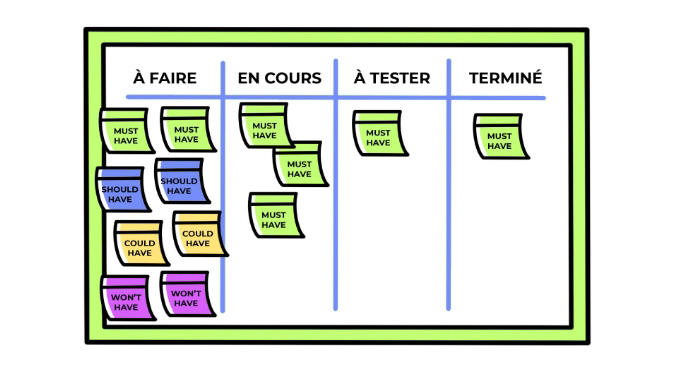
\includegraphics[width=0.8\textwidth]{methodeAgile.jpeg}
		\caption[Méthode agile Kanban en image]{Méthode agile Kanban en image\footnotemark}
		\label{fig:mon_label}
	\end{figure}
	\footnotetext{Source: openclassrooms}
	
	\section*{Conclusion}
	
	Ce chapitre a permis de situer le cadre institutionnel et
	probl\'ematique du pr\'esent travail. La pr\'esentation du
	\gls{minepat} a mis en \'evidence le r\^ole de cette institution
	dans la d\'efinition et la mise en \oe uvre des politiques
	\'economiques nationales. L'analyse du contexte a r\'ev\'el\'e
	que les initiatives men\'ees jusqu'ici pour documenter la situation
	des entreprises camerounaises pr\'esentent des limites communes~:
	elles ne couvrent pas l'ensemble du tissu productif et ne proposent
	pas de m\'ecanisme de mise en relation fond\'e sur les besoins
	exprim\'es. L'enqu\^ete du \gls{minepat} de 2025 constitue une
	r\'eponse institutionnelle \`a ces lacunes. Le chapitre suivant
	d\'efinit les concepts mobilis\'es dans ce travail et examine
	les solutions existantes de cartographie et de mise en relation.
	%============================================================
	%  CHAPITRE 2 : CONCEPTS ET ÉTAT DE L'ART
	%============================================================
	\chapter{Définition des concepts et état de l’art}
	Ce chapitre pose les fondements conceptuels et analytiques du
	travail. Il est organis\'e en deux parties~: la premi\`ere
	d\'efinit les notions de besoins des entreprises, de cartographie
	et de mise en relation~; la seconde examine les travaux et outils
	existants traitant de ces probl\'ematiques, en identifiant leurs
	apports et leurs limites au regard des objectifs poursuivis.
	\label{chap:etat_art}
	\newpage
	
	\section{Définition des concepts }
	\label{sec:concepts}
	
	\subsection{Cartographie des besoins des entreprises}
	
	Dans la litt\'erature \'economique, la notion de besoin renvoie \`a
	un \'ecart mesurable entre un \'etat observ\'e et un \'etat souhait\'e
	pour le bon fonctionnement d'une organisation. La Banque Mondiale
	d\'efinit les besoins des entreprises comme l'ensemble des contraintes
	qui, une fois lev\'ees, permettraient d'am\'eliorer de mani\`ere
	significative leur productivit\'e et leur capacit\'e \`a cro\^itre
	\cite{world_bank_doing_business_2020}. Cette d\'efinition s'inscrit
	dans le cadre m\'ethodologique de l'\textit{\'Evaluation des Besoins}
	(\textit{Needs Assessment}), une d\'emarche structur\'ee qui vise \`a
	identifier, hi\'erarchiser et documenter les manques d'une organisation
	afin d'orienter les interventions vers les facteurs de blocage les plus
	d\'eterminants \cite{world_bank_needs_2014}.
	
	La cartographie des besoins des entreprises est un processus
	syst\'ematique de collecte, d'organisation et de repr\'esentation
	sectorielle des contraintes exprim\'ees par les unit\'es
	\'economiques d'un territoire donn\'e. Elle constitue la premi\`ere
	\'etape op\'erationnelle d'une d\'emarche d'\'Evaluation des Besoins
	au sens de la Banque Mondiale, dont l'objectif est de produire une
	base d'information structur\'ee permettant aux d\'ecideurs publics
	d'orienter leurs interventions vers les entreprises et les contraintes
	les plus prioritaires \cite{world_bank_needs_2014}.
	
	
	\subsection{Mise en relation des entreprises}
	
La mise en relation des entreprises renvoie au mécanisme par lequel deux ou plusieurs unités économiques sont amenées à se connaître, à échanger sur leurs capacités et leurs besoins respectifs, et à explorer les conditions d'une collaboration mutuellement bénéfique. Il convient d'emblée de distinguer cette notion de celle de partenariat, avec laquelle elle est souvent confondue. La mise en relation constitue une étape préalable et distincte du partenariat proprement dit : tandis que la première relève d'un processus d'identification et de rapprochement entre acteurs économiques, le second renvoie à un accord formel ou tacite entre deux entreprises en vue d'une collaboration effective, généralement matérialisé par un contrat ou un protocole d'accord. Autrement dit, la mise en relation crée les conditions favorables à l'émergence d'un partenariat, sans pour autant le présupposer ni l'imposer. 
La mise en relation des entreprises constitue un facteur clé de renforcement des capacités productives et de génération de valeur. Elle permet en effet à une entreprise confrontée à un manque spécifique qu'il s'agisse d'un besoin en financement, en compétences techniques, en équipements ou en accès aux marchés de trouver un partenaire disposant précisément des ressources ou des capacités susceptibles de combler ce manque. L'Organisation de Coopération et de Développement Économiques (OCDE) souligne d'ailleurs que les dispositifs institutionnels de mise en relation contribuent significativement à l'amélioration de la productivité des petites et moyennes entreprises et à leur intégration dans les chaînes de valeur nationales et internationales \cite{ocde2021}. Plusieurs mécanismes et approches concourent à cette mise en relation entre entreprises, dont les principaux sont présentés ci-après.
	
	\subsubsection{Plateformes numériques B2B}
	Les plateformes numériques B2B (Business-to-Business) constituent l'une des formes les plus modernes et les plus répandues de mise en relation entre entreprises. Elles proposent un espace numérique dynamique où les entreprises peuvent se rendre visibles, interagir et engager des échanges commerciaux avec d'autres acteurs économiques, qu'ils soient nationaux ou internationaux \cite{acceor2024}. Contrairement aux marketplaces grand public, qui visent principalement les transactions entre professionnels et consommateurs, les plateformes B2B sont spécifiquement conçues pour faciliter les interactions entre entreprises, en soutenant aussi bien la prospection passive — consistant à attirer des partenaires potentiels grâce à une présence en ligne structurée — que la prospection active, fondée sur la recherche ciblée d'entreprises répondant à des critères sectoriels, géographiques ou fonctionnels précis. Elles jouent un rôle clé dans la quête de croissance et de réussite des entreprises en leur permettant d'élargir significativement leur réseau de partenaires au-delà des contraintes géographiques traditionnelles, de renforcer leur visibilité sur des marchés auxquels elles n'auraient pas accès autrement, et de fluidifier les échanges d'informations entre acteurs économiques évoluant dans un même secteur d'activité ou dans des secteurs complémentaires. Dans un contexte de numérisation croissante des économies africaines, ce type de dispositif représente une opportunité particulièrement prometteuse pour les entreprises camerounaises, dont la visibilité et la capacité de mise en réseau demeurent aujourd'hui limitées par l'absence d'un espace numérique institutionnel dédié.
	\subsubsection{Bourse de Sous Traitance et de Partenariat}
	
	Les Bourses de Sous-Traitance et de Partenariat (BSTP) constituent un autre mécanisme structuré de mise en relation entre entreprises, développé notamment en collaboration avec l'Organisation des Nations Unies pour le Développement Industriel (ONUDI) et le Programme des Nations Unies pour le Développement (PNUD). Ce sont des centres d'information technique, de promotion et de mise en relation entre donneurs d'ouvrages, fournisseurs et sous-traitants, dont la vocation première est de favoriser l'utilisation la plus optimale des capacités productives des industries affiliées \cite{minpmeesa}. Les bourses de sous-traitance jouent un double rôle dans l'écosystème économique : d'une part, elles fonctionnent comme des points de rencontre structurés entre l'offre et la demande de travaux de sous-traitance industrielle, mettant en relation des entreprises donneuses d'ordres avec des sous-traitants disposant des capacités requises ; d'autre part, elles assurent une fonction d'assistance et d'accompagnement, particulièrement à l'égard des petits et moyens sous-traitants ou fournisseurs qui disposent de moyens limités pour prospecter de manière autonome. L'objectif principal de ces structures est de fournir aux entreprises locales manufacturières les outils et les services qui amélioreront leurs performances et leurs pratiques, et qui leur permettront d'accéder à des marchés de sous-traitance industrielle auxquels elles n'auraient pas pu prétendre seules. Ce modèle présente une pertinence particulière dans le contexte camerounais, où la grande majorité des entreprises sont des très petites ou petites entreprises dont les capacités de prospection commerciale sont structurellement limitées.
	\subsubsection{Partenariats contractuels directs}
	Les partenariats contractuels directs représentent la forme la plus formalisée et la plus ancienne de mise en relation entre entreprises. Ils reposent sur un accord juridiquement contraignant entre deux ou plusieurs parties, qui définit les droits et obligations de chacune dans le cadre d'une collaboration spécifique. Ce type de partenariat peut intervenir à différentes étapes de la chaîne de valeur : dans l'activité de production, sous la forme de contrats de sous-traitance par lesquels une entreprise confie à une autre la réalisation d'une partie de sa production ; dans la distribution, via des accords d'exclusivité territoriale ou des contrats de franchise qui permettent à une entreprise de commercialiser les produits ou services d'une autre sur un marché donné ; ou encore dans le domaine de la recherche et de l'innovation, à travers des accords de co-développement ou de partage de propriété intellectuelle. Le contrat constitue l'instrument juridique le plus fréquemment utilisé pour matérialiser ces partenariats, la liberté contractuelle permettant aux parties de définir librement le contenu de leur accord en fonction de leurs besoins spécifiques et des contraintes de leur environnement \cite{williamson1985}. Si cette forme de partenariat offre une sécurité juridique importante, elle suppose en revanche une connaissance préalable des partenaires potentiels et un processus de négociation souvent long et coûteux, ce qui en limite l'accessibilité pour les petites structures disposant de ressources juridiques et financières limitées.
	\section{État de l'art}
	\label{sec:etat_art}
	
	\subsection{Enquêtes en vue de la cartographie des besoins des entreprises}
	Comme indiqué dans la problématique, plusieurs études ont été initiées dans l'optique de s'enquérir de la santé de l'écosystème du secteur privé camerounais en vue d'apporter des réformes permettant l'amélioration du climat des affaires. Ces initiatives, bien que pertinentes chacune dans son domaine, présentent des limites qui justifient la mise en place d'une solution plus intégrée. La présente section en propose une lecture analytique, en examinant successivement leurs objectifs, leur méthodologie, leurs principaux résultats et les lacunes qu'elles laissent subsister.\\
	
	\subsubsection{Enquete du GECAM}
	Le Groupement des Entreprises du Cameroun (GECAM) a initié en 2020 une enquête dont l'objectif était d'effectuer un état des lieux des entreprises qui composent le groupement et d'évaluer les difficultés auxquelles elles sont confrontées. La méthodologie retenue a consisté en une collecte de données directement auprès des entreprises membres, suivie du calcul de statistiques descriptives permettant d'évaluer leurs performances. Les résultats révèlent qu'en 2019, 57\% des entreprises du groupement ont connu des difficultés, la fiscalité étant identifiée comme le principal frein, caractérisée par l'instabilité du système fiscal (72\%), les pénalités et amendes fiscales (66\%), le niveau du taux d'imposition (61\%) et la multiplicité des contrôles de l'administration fiscale (59\%) \cite{gecam2019}. Toutefois, cette étude présenterait deux limites majeures: d'une part, elle se restreint aux seules  entreprises membres du GECAM, ne permettant pas de tirer des conclusions généralisables à l'ensemble du tissu économique national; d'autre part, aucune recommandation concrète n'a été formulée à l'endroit des entreprises, et la question des besoins spécifiques et des opportunités de partenariat n'y est pas abordée.\\
	
	\begin{figure}[H]           % H = ici exactement
		\centering
		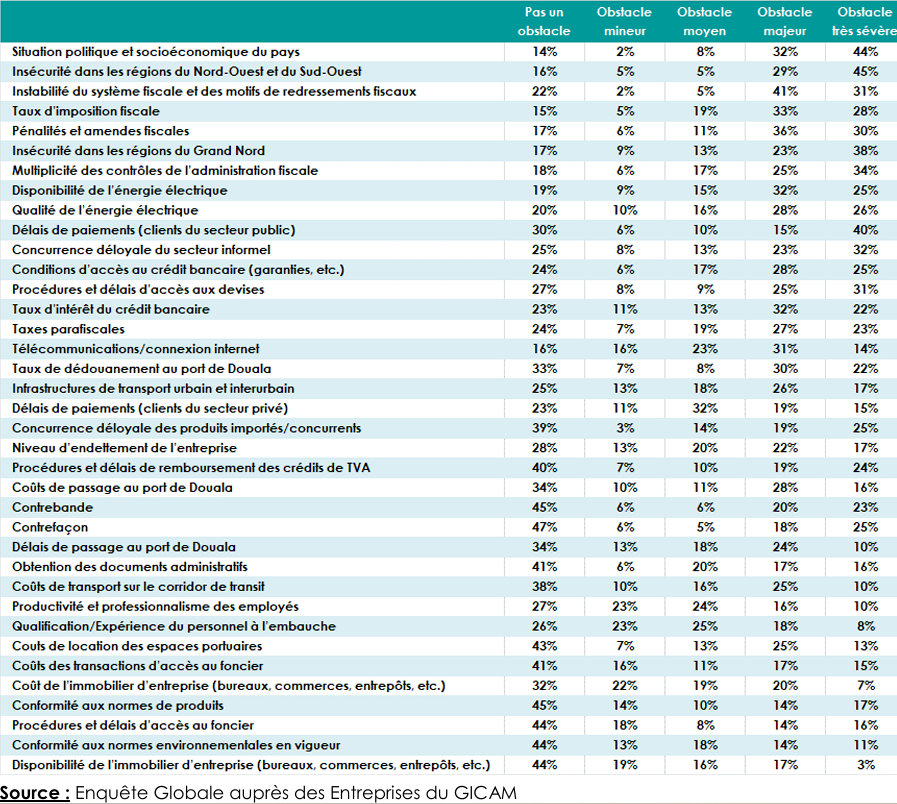
\includegraphics[width=0.8\textwidth]{enqueteGecam.png}
		\caption{récapitulatif de l'enquête du GECAM}
		\label{fig:mon_label}
	\end{figure}
	
	\subsubsection{Redaction du document de stratégie pour le developpement du secteur industriel par le MINEPAT}
	En 2022, le MINEPAT a engagé la rédaction d'un document de stratégie visant à proposer un nouveau cadre stratégique pour le secteur industriel, en réalignant la Stratégie de Développement du Secteur de l'Industrie et des Services (SDSIS) sur la planification post-Document Stratégique pour la Croissance Économique (DSCE). La démarche méthodologique adoptée s'est articulée en trois étapes: un état des lieux préalable de l'industrie camerounaise, une identification des problèmes susceptibles d'entraver le développement du secteur, et la proposition de stratégies assorties de mécanismes d'évaluation et de suivi. Les principaux résultats indiquent que la part de la valeur ajoutée manufacturière dans le PIB stagnait à 14,08\% en 2015, loin derrière des pays comparables tels que la Thaïlande (28,6\%) et la Malaisie (24\%); que 90\% des entreprises locales sont des très petites, petites ou moyennes entreprises; et que des projets structurants tels que le projet FABER et la construction de 8,000 km de voies ferrées ont été envisagés pour redynamiser le secteur \cite{minepat2022}. Les limites de ce document sont cependant notables: centré sur le seul secteur industriel, il n'évoque ni les besoins spécifiques des entreprises, ni les opportunités de partenariat inter-entreprises qui constituent pourtant un levier essentiel de compétitivité. \\
	
\subsubsection{Enquete sur le climat des affaires par le MINEPAT}
	Dans la continuité de ces travaux, le MINEPAT a lancé en novembre 2023 une enquête visant à préciser la manière dont les entreprises du secteur industriel perçoivent le climat des affaires, notamment en matière d'accès au financement, d'accès aux marchés et d'accès aux facteurs de production, ainsi que les actions menées par l'État en vue de l'améliorer. Sur le plan méthodologique, un échantillon de 1,000 entreprises a été constitué à l'échelle nationale en s'appuyant sur le réseau des délégués régionaux et départementaux du \gls{minepat}. Un questionnaire en ligne a été soumis, l'apurement et l'analyse des données collectées ont été effectués. Les résultats indiquent que 91\% des chefs d'entreprises considèrent que les coûts liés au taux d'intérêt, aux assurances et au courtage sont trop élevés, et appellent l'État à mettre en place des structures dédiées au financement des entreprises. L'accès aux facteurs de production et l'état des infrastructures routières sont unanimement identifiés comme des freins majeurs à la croissance. Malgré ces apports, l'étude reste circonscrite au seul secteur industriel et ne propose aucun mécanisme concret de mise en relation entre entreprises pour répondre aux besoins identifiés. \\
	
	\subsubsection{Recensement Général des Entreprises par l'INS}
	Enfin, le troisième Recensement Général des Entreprises (RGE3), réalisé par l'Institut National de la Statistique en 2023, avait pour objectifs d'actualiser le fichier des unités économiques nationales, de mettre en place un Système d'Information Géographique des entreprises et d'effectuer une analyse comparative avec les précédents recensements \cite{ins2023}. La méthodologie a consisté à constituer un fichier de base à partir des données administratives disponibles auprès de la Direction Générale des Impôts (DGI) et de la Caisse Nationale de Prévoyance Sociale (CNPS), puis à procéder à une collecte de terrain à l'aide d'outils numériques, après découpage du territoire national en douze Zones de Recensement \cite{ins2023}. Les résultats mettent en évidence une croissance significative du tissu entrepreneurial entre 2016 et 2023, avec une hausse de 109,5\% du nombre d'unités économiques, une prédominance du secteur tertiaire représentant 85,6\% des unités recensées, et une concentration très marquée des entreprises individuelles qui représentent 92,4\% du total. Cependant, en dépit de l'envergure de cet exercice, les défis rencontrés par les entreprises et leurs besoins spécifiques n'ont pas été documentés, et aucun outil de mise en relation entre acteurs économiques complémentaires n'a été envisagé à l'issue du recensement.\\
	
	\begin{figure}[H]           % H = ici exactement
		\centering
		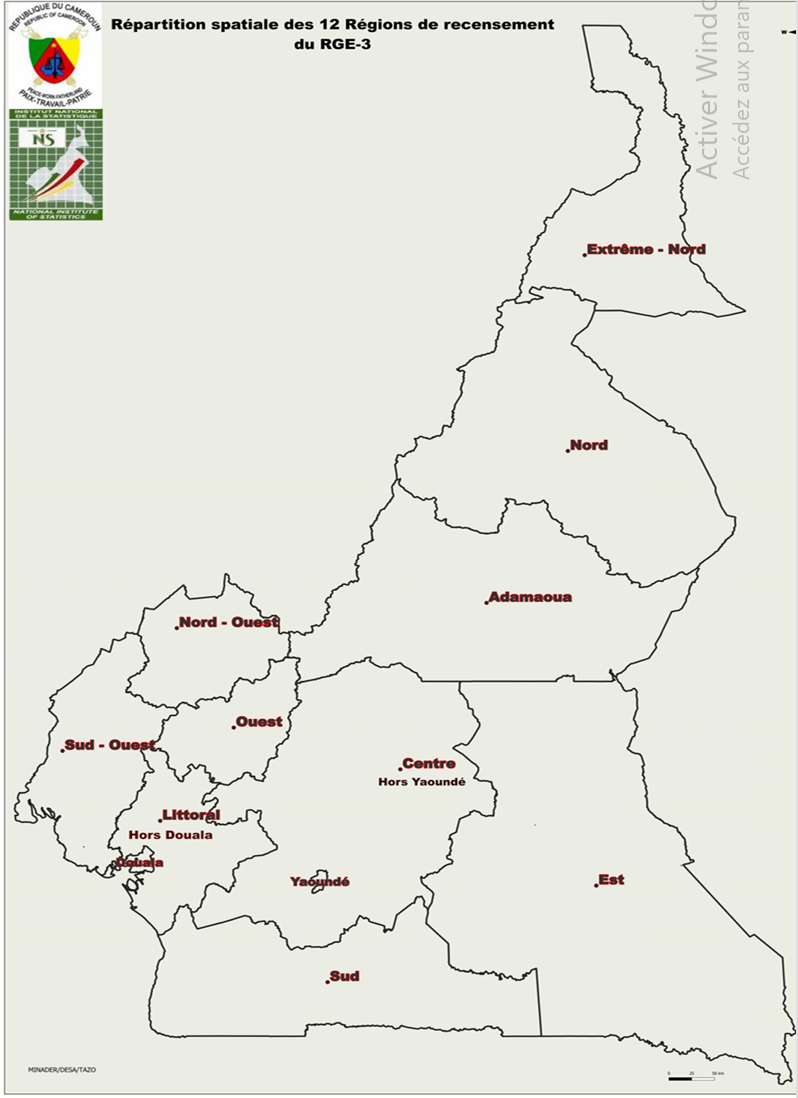
\includegraphics[width=0.8\textwidth]{zoneRecensement.png}
		\caption[Découpage des zones de recensement]{Découpage des zones de recensement \footnotemark}
		\label{fig:zoneResencement}
	\end{figure}
	\footnotetext{Source : Rapport du $3^{\text{eme}}$ Recensement Général des Entreprises}
\subsection{\'Etat de l'art}
\label{sec:etat_art}

\subsubsection{Syst\`emes de recommandation et mise en relation
	d'entreprises}

Les syst\`emes de recommandation constituent la cat\'egorie de
solutions algorithmiques la plus directement li\'ee au probl\`eme
trait\'e dans ce travail. Selon Francesco Ricci et all., ces syst\`emes
peuvent \^etre class\'es en trois familles selon leur principe de
fonctionnement \cite{ricci_2015}.

Le \textbf{filtrage bas\'e sur le contenu} (\textit{content-based
	filtering}) propose \`a un utilisateur des \'el\'ements pr\'esentant
des attributs similaires \`a ceux avec lesquels il a d\'ej\`a
interagi. Appliqu\'e \`a la mise en relation d'entreprises, ce
principe conduit \`a rapprocher des entreprises dont les profils
de besoins sont similaires. Sa limite principale est qu'il ne prend
pas en compte la compl\'ementarit\'e entre offres et besoins~: deux
entreprises ayant les m\^emes besoins ne sont pas n\'ecessairement
celles qui peuvent se r\'epondre mutuellement.

Le \textbf{filtrage collaboratif} (\textit{collaborative filtering})
exploite les comportements collectifs des utilisateurs pour inf\'erer
des affinit\'es. Dans le contexte B2B, il suppose l'existence d'un
historique d'interactions entre entreprises, ce qui est rarement
disponible dans les contextes institutionnels africains o\`u les
donn\'ees transactionnelles sont peu structur\'ees \cite{ricci_2015}.

Les \textbf{syst\`emes \`a base de connaissances}
(\textit{knowledge-based systems}) font correspondre les contraintes
d'un utilisateur avec les caract\'eristiques des \'el\'ements
disponibles. C'est l'approche la plus proche du probl\`eme trait\'e
dans ce travail~: l'entreprise exprime ses besoins et la plateforme
identifie les entreprises capables d'y r\'epondre. L'on peut
noter que cette approche ne souffre pas du probl\`eme du
\textit{cold start} (absence d'historique), ce qui la rend
particuli\`erement adapt\'ee aux contextes o\`u les donn\'ees
d'interaction sont rares.

\subsubsection{Plateforme de mise en relation~:
	travaux existants}

Plusieurs travaux acad\'emiques et institutionnels ont abord\'e la
probl\'ematique de la mise en relation d'entreprises dans les pays
en d\'eveloppement. \cite{lu_zhou_2011} ont propos\'e un cadre de
\textit{link prediction} sur des graphes bipartites offre-demande,
montrant que la structure de voisinage dans un r\'eseau \'economique
permet de pr\'edire avec une pr\'ecision \'elev\'ee les partenariats
potentiels entre entreprises. Cette approche a \'et\'e appliqu\'ee
avec succ\`es dans des contextes de sous-traitance industrielle en
Am\'erique latine, o\`u les Bourses de Sous-Traitance et de
Partenariat (BSTP) ont permis d'augmenter le taux d'utilisation
des capacit\'es productives des PME de 15 \`a 30\,\% dans les
secteurs participants \cite{unido_2022}.

Dans le contexte africain, la Commission \'Economique pour l'Afrique
souligne que l'absence de dispositifs institutionnels num\'eriques
de mise en relation constitue l'un des principaux obstacles \`a
l'int\'egration des PME dans les cha\^ines de valeur r\'egionales
\cite{uneca_digital_2023}. Cette lacune est aggravel'absence de
bases de donn\'ees structur\'ees sur les besoins et les capacit\'es
des entreprises locales, que les recensements existants --- comme
le \gls{rge}3 --- ne comblent pas enti\`erement \cite{ins2023}.

\subsubsection{Limites des plateformes commerciales existantes}

Les plateformes commerciales de mise en relation (LinkedIn, Alibaba,
Facebook Marketplace, Go Africa Online) pr\'esentent des limites
communes au regard des objectifs institutionnels poursuivis dans ce
travail. Premi\`erement, leur algorithme de recommandation repose
sur des signaux comportementaux (clics, vues, interactions) qui
pr\'esupposent un historique d'utilisation inexistant pour les
entreprises nouvellement enregistr\'ees \cite{ricci_2015}.
Deuxi\`emement, ces plateformes sont con\c{c}ues pour des
transactions commerciales et non pour la mise en correspondance
offre-demande sur la base de besoins d\'eclar\'es.
Troisi\`emement, leur mod\`ele \'economique fond\'e sur des
abonnements payants exclut de facto les entreprises \`a faibles
ressources, qui constituent pourtant la majorit\'e du tissu
productif camerounais \cite{ins2023}.
\section*{Conclusion}
Ce chapitre a permis de d\'elimiter le cadre conceptuel du travail
et de situer la contribution par rapport \`a l'existant. Les
d\'efinitions propos\'ees s'appuient sur le cadre m\'ethodologique
de l'\'Evaluation des Besoins de la Banque Mondiale, qui fournit
une base op\'erationnelle pour l'analyse des donn\'ees de l'enqu\^ete.
L'examen des travaux existants montre qu'aucune solution disponible
ne combine, dans un cadre institutionnel, la collecte structur\'ee
des besoins et un m\'ecanisme de mise en relation fond\'e sur ces
besoins. Le chapitre suivant pr\'esente le cahier des charges de
la plateforme \textit{Business Partnership}, qui r\'epond
pr\'ecis\'ement \`a cette lacune.
	%============================================================
	%  CHAPITRE 3 : MÉTHODOLOGIE
	%============================================================
	%=============================================================
	\chapter{Cahier des charges de la plateforme
		\textit{Business Partnership}}
	\label{chap:cahier_charges}
	%=============================================================
	
Ce chapitre formalise les exigences de la plateforme
\textit{Business Partnership}. Il pr\'esente successivement le
p\'erim\`etre du projet, l'identification des acteurs, les
sp\'ecifications fonctionnelles et non fonctionnelles, les mod\`eles
de conception (\gls{uml}), et le mod\`ele de donn\'ees logique.
	
	%=============================================================
	\section{Périmètre du projet et identification des acteurs}
	\label{sec:contexte_projet}
	%=============================================================
	\subsection{Périmétre du projet}
	\subsubsection{Contexte institutionnel}
	
	La plateforme \textit{Business Partnership} s'inscrit dans le cadre
	de la mise en \oe uvre de la Stratégie Nationale de Développement
	2020--2030 (\gls{snd30}), qui identifie le développement du secteur
	privé comme l'un des leviers essentiels de la transformation
	structurelle de l'économie camerounaise. Elle constitue le
	prolongement numérique de l'enquête sur la cartographie et les
	besoins des entreprises conduite par le \gls{minepat} en 2025,
	dont les données collectées alimentent directement le moteur de mise en relation. La plateforme est
	destinée à être opérée sous la tutelle du \gls{minepat}, qui
	en assurera la gouvernance et la maintenance, et à être accessible
	à l'ensemble des entreprises du tissu productif camerounais
	disposant d'un accès à internet.
	
	\subsubsection{Périmètre fonctionnel}
	
	Le périmètre de la plateforme \textit{Business Partnership} couvre
	les fonctionnalités suivantes~:
	
	\begin{itemize}
		\item la création et la gestion de comptes d'entreprises~;
		\item la saisie des besoins exprimés par
		les entreprises~;
		\item la mise en relation automatisée des entreprises;
		\item l'administration et le suivi de la plateforme par les
		agents du \gls{minepat}.
	\end{itemize}
	
	
	%=============================================================
	%\section{Identification des acteurs}
	%\label{sec:acteurs}
	%=============================================================
	\subsection{Identifications des acteurs}
	L'identification précise des acteurs du système constitue un
	préalable indispensable à la définition des cas d'usage et à la
	modélisation des droits d'accès. Un acteur est défini ici comme
	toute entité --- humaine ou système externe --- qui interagit
	avec la plateforme \textit{Business Partnership} dans le cadre
	de son utilisation normale. Trois catégories d'acteurs principaux
	ont été identifiées.
	
	
	\subsubsection{L'entreprise (acteur principal)}
	
	L'entreprise constitue l'acteur central de la plateforme. Elle
	désigne toute unité économique --- quelle que soit sa taille,
	sa forme juridique ou son secteur d'activité --- qui s'inscrit
	sur la plateforme afin de renseigner son profil, d'exprimer
	ses besoins et de consulter les recommandations de partenaires
	potentiels générées par le moteur de mise en relation. L'entreprise
	est représentée sur la plateforme par un  utilisateur
	physique disposant d'un compte personnel sécurisé.
	
	\subsubsection{L'administrateur}
	
	L'administrateur est un agent du \gls{minepat} disposant de
	droits d'accès étendus à l'ensemble des fonctionnalités de la
	plateforme. Il est chargé de la validation des inscriptions des
	entreprises, du suivi
	des indicateurs d'utilisation et de l'administration technique
	de la plateforme. Il dispose d'un tableau de bord dédié lui
	permettant de superviser en temps réel l'ensemble des activités
	de la plateforme.
	
	\subsubsection{Le visiteur}
	
	Le visiteur désigne tout internaute qui accède à la plateforme
	sans être authentifié. Il peut consulter les informations
	publiques de présentation de la plateforme et ses fonctionnalités,
	mais ne peut accéder ni aux profils des entreprises, ni aux
	recommandations, ni à aucune fonctionnalité interactive. Son
	accès est strictement limité aux pages publiques, afin de
	protéger la confidentialité des informations des entreprises
	enregistrées.
	
	\begin{table}[H]
		\centering
		\caption{Synthèse des acteurs et de leurs droits d'accès}
		\label{tab:acteurs}
		\renewcommand{\arraystretch}{1.5}
		\begin{tabularx}{\textwidth}{>{\raggedright\arraybackslash}p{3cm}
				>{\centering\arraybackslash}p{2.2cm}
				>{\centering\arraybackslash}p{2.2cm}
				>{\centering\arraybackslash}X}
			\toprule
			\rowcolor{primary!15}
			\textbf{Fonctionnalité}
			& \textbf{Visiteur}
			& \textbf{Entreprise}
			& \textbf{Administrateur} \\
			\midrule
			
			\rowcolor{lightgray}
			Créer un compte entreprise
			& \textcolor{green!60!black}{\checkmark}
			& \textcolor{green!60!black}{\checkmark}
			& \textcolor{green!60!black}{\checkmark} \\
			
			Gérer son profil
			& \textcolor{accent}{\texttimes}
			& \textcolor{green!60!black}{\checkmark}
			& \textcolor{green!60!black}{\checkmark} \\
			
			\rowcolor{lightgray}
			Saisir ses besoins
			& \textcolor{accent}{\texttimes}
			& \textcolor{green!60!black}{\checkmark}
			& \textcolor{green!60!black}{\checkmark} \\
			
			Consulter les recommandations
			& \textcolor{accent}{\texttimes}
			& \textcolor{green!60!black}{\checkmark}
			& \textcolor{green!60!black}{\checkmark} \\
			
			\rowcolor{lightgray}
			Contacter un partenaire
			& \textcolor{accent}{\texttimes}
			& \textcolor{green!60!black}{\checkmark}
			& \textcolor{green!60!black}{\checkmark} \\
			
			\rowcolor{lightgray}
			Accéder au tableau de bord
			& \textcolor{accent}{\texttimes}
			& \textcolor{accent}{\texttimes}
			& \textcolor{green!60!black}{\checkmark} \\
			
			Gérer les utilisateurs
			& \textcolor{accent}{\texttimes}
			& \textcolor{accent}{\texttimes}
			& \textcolor{green!60!black}{\checkmark} \\
			
			\rowcolor{lightgray}
			Exporter les données
			& \textcolor{accent}{\texttimes}
			& \textcolor{accent}{\texttimes}
			& \textcolor{green!60!black}{\checkmark} \\
			
			\bottomrule
		\end{tabularx}
	\end{table}
	
	%=============================================================
	\section{Spécifications fonctionnelles et non fonctionnelles}
	\label{sec:specs_fonctionnelles}
	%=============================================================
	\subsection{Spécifications fonctionnelles}
	Les spécifications fonctionnelles décrivent de manière exhaustive
	et précise l'ensemble des fonctionnalités que doit offrir la
	plateforme \textit{Business Partnership} à ses différents acteurs.
	Chaque fonctionnalité est décrite sous la forme d'un cas d'usage
	(\textit{use case}), précisant les acteurs impliqués, les
	préconditions, le scénario nominal et les exceptions éventuelles.
	
	\subsubsection{Gestion des comptes et authentification}
	
	
		\textbf{Acteur principal~:} Représentant légal de l'entreprise \\
		\textbf{Préconditions~:} L'entreprise n'est pas encore enregistrée
		sur la plateforme \\
		\textbf{Scénario nominal~:}
		\begin{itemize}
			\item L'utilisateur accède au formulaire d'inscription depuis
			la page d'accueil de la plateforme~;
			\item Il renseigne les informations obligatoires~: raison sociale,
			statut juridique, région, secteur d'activité, adresse
			électronique et mot de passe, documents; 
			\item Il soumet le formulaire~;
			\item Le système vérifie la validité et la cohérence des
			informations saisies~;
			\item L'administrateur de la plateforme examine les informations envoyées et valide ou invalide la création du compte.
		\end{itemize}
		\textbf{Exceptions~:} Adresse électronique déjà utilisée~;
		informations incomplètes ou incohérentes.
	
	
	\vspace{0.5cm}
	
		\textbf{Acteur principal~:} Entreprise / Administrateur \\
		\textbf{Préconditions~:} L'utilisateur dispose d'un compte validé \\
		\textbf{Scénario nominal~:}
		\begin{itemize}
			\item L'utilisateur saisit son nom d'utilisateur et son
			mot de passe dans le formulaire de connexion~;
			\item Le système vérifie les identifiants~;
			\item En cas de succès, l'utilisateur est redirigé vers son
			tableau de bord personnel.
		\end{itemize}
		\textbf{Exceptions~:} Identifiants incorrects.

	
	\subsubsection{Gestion des besoins}
	
		\textbf{Acteur principal~:} Entreprise \\
		\textbf{Préconditions~:} Le profil de l'entreprise est complété
		à au moins 50\,\% \\
		\textbf{Scénario nominal~:}
		\begin{enumerate}
			\item L'utilisateur accède à la secttion définir mes besoins automatiquement après l'enregistrement;
			\item Il défini ses besoins par services;
			\item Il défini également ses offres par service;
			\item La mise en relation se fait instantanément sur la base des entreprises déjà enregistrées.
		\end{enumerate}
		
\subsubsection{Administration de la plateforme}
	

	\textbf{Acteur principal :} Administrateur \par\smallskip
	\textbf{Préconditions :} L'administrateur est authentifié avec ses droits étendus \par\smallskip
	\textbf{Scénario nominal :}
	\begin{itemize}
		\item L'administrateur accède à son tableau de bord dédié ;
		\item Il consulte les indicateurs clés de la plateforme :
		nombre d'entreprises enregistrées, nombre de besoins
		saisis, nombre de mises en relation initiées;
		\item Il valide ou invalide une demande d'adhésion;
		\item Il accède à la liste complète des entreprises et peut
		consulter, modifier ou suspendre tout profil.
	\end{itemize}

	%=============================================================
	%\section{Spécifications non fonctionnelles}
	%\label{sec:specs_non_fonctionnelles}
	%=============================================================
	\subsection{Spécifications non fonctionnelles}
	Les spécifications non fonctionnelles définissent les contraintes
	de qualité, de performance et de sécurité auxquelles la plateforme
	\textit{Business Partnership} doit se conformer, indépendamment
	des fonctionnalités qu'elle offre. Elles constituent des exigences
	transversales qui conditionnent la qualité globale de la solution
	et son adéquation aux contraintes du contexte camerounais.
	
	%\subsection{Exigences de performance}
	
	
	\subsubsection{Exigences de sécurité}
	
	La sécurité constitue une exigence fondamentale de la plateforme,
	en raison de la sensibilité des informations économiques et
	commerciales que les entreprises y déposent. Les mesures de
	sécurité suivantes sont imposées~:
	
	\begin{itemize}
		
		\item \textbf{Hachage des mots de passe}~: les mots de passe
		des utilisateurs doivent être stockés sous forme hachée à l'aide
		d'un algorithme cryptographiquement sûr,
		et ne doivent en aucun cas être stockés en clair dans la base
		de données~;
		
		\item \textbf{Protection contre les attaques courantes}~: la
		plateforme doit intégrer des mécanismes de protection contre
		les principales vulnérabilités web répertoriées par l'\gls{owasp}, notamment les
		injections SQL, les attaques par script intersite (XSS) et
		la falsification de requêtes intersites (CSRF). Le framework
		Django, retenu pour le développement, intègre nativement des
		mécanismes de protection contre ces attaques~;
		
		\item \textbf{Contrôle d'accès}~: un système de contrôle
		d'accès basé sur les rôles (\textit{Role-Based Access Control},
		RBAC) doit garantir qu'aucun utilisateur ne peut accéder à des
		ressources ou des fonctionnalités au-delà de celles autorisées
		par son profil~;
		
		\item \textbf{Journalisation des accès}~: les accès à la
		plateforme et les opérations sensibles (modification de profil,
		suppression de données, connexions administrateur) doivent
		être journalisés afin de permettre la traçabilité et l'audit.
	\end{itemize}
	
	\subsubsection{Exigences d'accessibilité et d'ergonomie}
	
	La plateforme doit être accessible depuis les navigateurs web
	modernes les plus répandus (Google Chrome, Mozilla Firefox,
	Microsoft Edge, Safari) dans leurs versions récentes, sans
	nécessiter l'installation de plugins ou d'extensions tierces.
	Elle doit adopter une conception \textit{responsive}, garantissant
	une expérience utilisateur satisfaisante aussi bien sur ordinateur
	de bureau que sur terminal mobile, ces derniers représentant le
	principal mode d'accès à internet pour une large fraction des
	utilisateurs camerounais. L'interface doit être rédigée intégralement
	en \textbf{langue française}.
	

	%=============================================================
	\subsubsection{Diagramme des cas d'usage}
	\label{sec:use_case}
	%=============================================================
	
	Le diagramme des cas d'usage synthétise l'ensemble des interactions
	entre les acteurs identifiés et les fonctionnalités de la plateforme.
	Il constitue une représentation graphique standardisée, issue de la
	notation UML (\textit{Unified Modeling Language}), qui permet de
	communiquer de manière claire et non ambiguë les exigences
	fonctionnelles du système à l'ensemble des parties prenantes du
	projet, qu'elles soient techniques ou non \citep{booch_1998}.
	\begin{figure}[htbp]
		\centering
		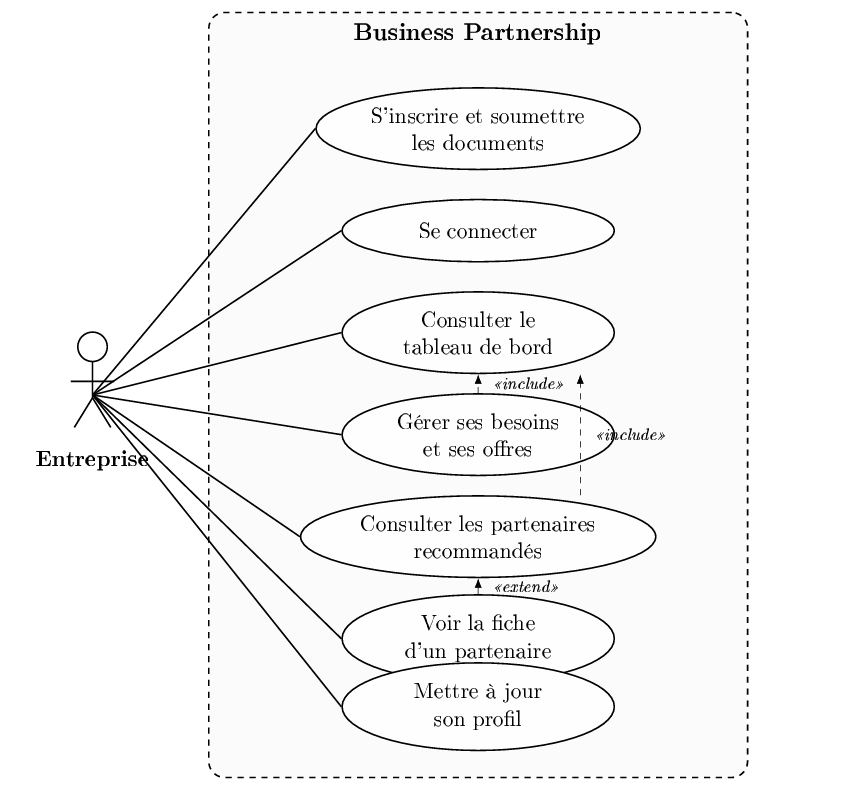
\includegraphics[width=0.85\textwidth]{UseCase1.png}
		\caption{Diagramme de cas d'utilisation -- Vue Entreprise}
		\label{fig:uc_entreprise}
	\end{figure}
	
	\begin{figure}[htbp]
		\centering
		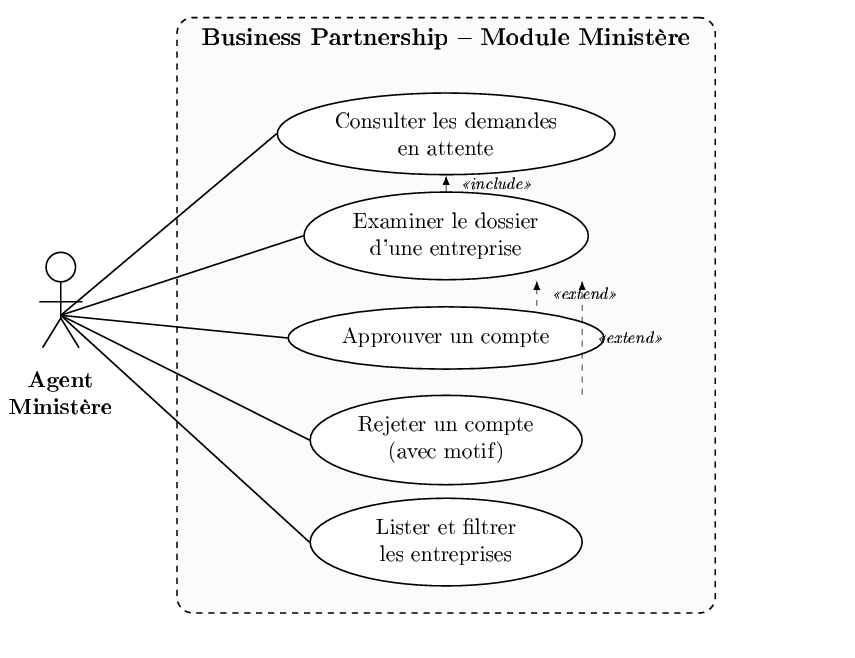
\includegraphics[width=0.85\textwidth]{UseCase2.png}
		\caption{Diagramme de cas d'utilisation -- Vue Agent Minist\`ere}
		\label{fig:uc_agent}
	\end{figure}
	
	\subsection{Architecture logicielle}
	\label{subsec:architecture_logicielle}
	
	La plateforme \textit{Business Partnership} suit le patron
	d'architecture \textbf{MVT} (Mod\`ele-Vue-Template) de Django,
	qui s\'epare la logique de donn\'ees, la logique m\'etier et la
	couche de pr\'esentation. La figure~\ref{fig:architecture_logicielle}
	illustre les interactions entre les composantes du syst\`eme.
	
	\begin{figure}[H]
		\centering
		\begin{tikzpicture}[
			box/.style={rectangle, draw=black, fill=lightgray,
				text width=4cm, align=center,
				minimum height=1cm, font=\small},
			arr/.style={->, thick}
			]
			\node[box] (client)  at (0,   4) {Navigateur web \\ (Client HTTP)};
			\node[box] (url)     at (0,   2.2) {URL Dispatcher \\ (urls.py)};
			\node[box] (vue)     at (0,   0.4) {Vue \\ (views.py)};
			\node[box] (modele)  at (-3.5,-1.4) {Mod\`ele \\ (models.py + ORM)};
			\node[box] (db)      at (-3.5,-3.2) {Base de donn\'ees \\ (SQLite3)};
			\node[box] (template)at ( 3.5,-1.4) {Template \\ (HTML + Bootstrap)};
			\node[box] (reco)    at ( 3.5,-3.2) {Module de \\ mise en relation \\ (SQL)};
			
			\draw[arr] (client)   -- (url);
			\draw[arr] (url)      -- (vue);
			\draw[arr] (vue)      -- (modele);
			\draw[arr] (modele)   -- (db);
			\draw[arr] (db)       -- (modele);
			\draw[arr] (modele)   -- (vue);
			\draw[arr] (vue)      -- (template);
			\draw[arr] (template) -- (client);
			\draw[arr] (vue)      -- (reco);
			\draw[arr] (reco)     -- (vue);
		\end{tikzpicture}
		\caption{Architecture logicielle de la plateforme
			\textit{Business Partnership}}
		\label{fig:architecture_logicielle}
	\end{figure}
	
	\subsection{Limites de la plateforme}
	\label{subsec:limites}
	
	\subsubsection{Limites relatives aux donn\'ees}
	
	La base de donn\'ees de la plateforme est aliment\'ee par les
	donn\'ees de l'enqu\^ete du \gls{minepat} de 2025.
	Les entreprises du secteur informel, les microentreprises rurales
	et les structures non enregistr\'ees aupr\`es des d\'el\'egations
	du \gls{minepat} ne sont pas repr\'esent\'ees dans la base.
	Cela limite la couverture effective du moteur de recommandation~:
	une entreprise dont les partenaires potentiels ne sont pas
	enregistr\'es sur la plateforme ne recevra pas de recommandations
	pertinentes.
	
	\subsubsection{Limites du moteur de mise en relation}
	
	Le moteur de mise en relation actuel repose sur une correspondance
	directe entre besoins d\'eclar\'es et offres de services. Cette
	approche ne prend pas en compte la proximit\'e g\'eographique
	entre entreprises, ni la capacit\'e de production r\'eelle des
	entreprises offreuses. Par ailleurs, l'absence d'un m\'ecanisme
	de retour d'exp\'erience (\textit{feedback}) apr\`es une mise en
	relation ne permet pas d'am\'eliorer les recommandations au fil
	du temps.
	
	\subsubsection{Limites techniques}
	
	La base de donn\'ees SQLite3 retenue pour le prototype pr\'esente
	des limites de performance en cas d'acc\`es concurrents \'elev\'es.
	Son remplacement par PostgreSQL est n\'ecessaire avant tout
	d\'eploiement en production. De plus, la plateforme ne dispose pas
	d'interface en langue anglaise, ce qui limite son accessibilit\'e
	dans les r\'egions anglophones du Cameroun.
	
\section*{Conclusion}
	Ce chapitre a formalis\'e l'ensemble des exigences de la plateforme
	\textit{Business Partnership}, depuis les cas d'usage jusqu'aux
	mod\`eles de conception et au mod\`ele de donn\'ees logique. Les
	sp\'ecifications d\'efinies constituent la base sur laquelle repose
	le d\'eveloppement pr\'esent\'e au chapitre suivant, qui d\'ecrit
	les m\'ethodes d'analyse des donn\'ees et la mise en \oe uvre
	technique de la plateforme.
	
	
	\chapter{Cartographie des besoins, conception et modélisation de la plateforme}
	Il sera question dans ce chapitre de présenter premièrement la méthodologie utilisée en vue du traitement des données issues de  l’enquête réalisée par le MINEPAT sur la cartographie des besoins des entreprises. Nous débuterons par une présentation des données à travers la description de la source de données, des variables et en fin les méthodes de traitements de ces données. S’en suivra enfin la présentation de la conception de la plateforme gouvernementale et des techniques utilisées.
	\label{chap:methodo}
	
	\section{Méthodologie d'analyse pour la cartographie des besoins des entreprises}
	
	\subsection{Présentation des données}
	\subsubsection{Source de données}
	L’enquête réalisée par le MINEPAT plus précisément par la \gls{dape} s’est fait à travers la soumission d’un formulaire électronique par les entreprises cibles. De cette soumission une base de données a pu être constituée résultat des réponses des entreprises qui faisaient l’objet de l’enquête. Le traitement de ces données s’est effectué dans le strict respect des procédures et outils statistiques. Le fichier \textbf{identifications.csv} regroupe l'ensemble des informations permettant d'identifier et de caractériser les entreprises enquêtées. Il contient des variables relatives à la dénomination de l'entreprise, à sa localisation géographique, à son secteur d'activité, à sa forme juridique, à son année de création et à sa taille. Ce fichier constitue la dimension cartographique de la base de données, en ce qu'il permet de positionner chaque entreprise dans le tissu économique national selon plusieurs axes d'analyse. Le fichier \textbf{besoins.csv}, quant à lui, recense les besoins exprimés par les entreprises en réponse aux questions posées dans le formulaire. Il contient des informations sur les types de besoins identifiés par les entreprises qu'ils soient d'ordre financier, organisationnel, technologique ou commercial. Ce fichier constitue la dimension analytique de la base de données, sur laquelle repose la logique de recommandation de la plateforme.  Ces deux fichiers ont été joints par un identifiant unique attribué à chaque entreprise lors de la collecte, permettant d'associer à chaque unité économique ses caractéristiques d'identification et ses besoins exprimés. Avant toute analyse, une phase d'apurement des données a été réalisée afin de traiter les valeurs manquantes, d'identifier les doublons éventuels et de vérifier la cohérence des réponses fournies.
	\subsubsection{Description des variables}
	Les variables utilisées lors de cette enquête sont essentiellement qualitative et sont orientées dans deux buts principaux : identifier de la manière la plus précise possible les entreprises et obtenir des informations les plus complètes sur leurs besoins. Nous nous proposons de décrire ces variables dans les tableaux qui suivent.
	
	%------------------------------------------------------------------
	% Tableau 1 : Variables d'identification
	%------------------------------------------------------------------
	\begin{table}[H]
		\centering
		\caption{Variables pour l'identification des entreprises
			(\texttt{identifications.csv})}
		\label{tab:var_identification}
		\renewcommand{\arraystretch}{1.5}
		\begin{tabularx}{\textwidth}{
				>{\ttfamily\raggedright\arraybackslash}p{3.8cm}
				>{\raggedright\arraybackslash}p{2.8cm}
				>{\raggedright\arraybackslash}X}
			
			\toprule
			\rowcolor{primary!15}
			\textbf{Variable} & \textbf{Type} & \textbf{Commentaire} \\
			\midrule
			
			id
			& Qualitatif nominal
			& Entier attribué automatiquement par la plateforme en fonction
			de la date de soumission du formulaire. \\
			
			\rowcolor{lightgray}
			raison\_sociale
			& Qualitatif nominal
			& Permet d'obtenir la dénomination sous laquelle l'entreprise
			s'est enregistrée. \\
			
			statut\_juridique
			& Qualitatif nominal
			& Permet d'obtenir le statut juridique de l'entreprise
			(SARL, SA, EI, etc.). \\
			
			\rowcolor{lightgray}
			autre\_statut\_juridique
			& Qualitatif nominal
			& Champ de saisie libre permettant à l'entreprise d'indiquer
			son statut juridique lorsque celui-ci ne figure pas parmi
			les modalités proposées dans le formulaire. \\
			
			region
			& Qualitatif nominal
			& Permet d'identifier la région dans laquelle évolue
			l'entreprise parmi les dix régions du Cameroun. \\
			
			\rowcolor{lightgray}
			localisation
			& Qualitatif nominal
			& Permet d'obtenir des informations plus précises sur
			l'emplacement de l'entreprise, au niveau du quartier
			ou de la ville. \\
			
			taille\_entreprise
			& Qualitatif nominal
			& Fait référence aux différentes catégories d'entreprises
			rencontrées au Cameroun selon leur taille
			(TPE, PE, PME, GE). \\
			
			\rowcolor{lightgray}
			date\_debut\_activite
			& Qualitatif nominal
			& Renvoie à la date effective de démarrage des activités
			de l'entreprise. \\
			
			secteur\_activite
			& Qualitatif ordinal
			& Fait référence au secteur d'activité auquel appartient
			l'entreprise (primaire, secondaire ou tertiaire). \\
			
			\rowcolor{lightgray}
			secteur\_autre
			& Qualitatif ordinal
			& Champ de saisie libre permettant d'enregistrer un secteur
			d'activité autre que ceux proposés dans le formulaire. \\
			
			branche\_activite
			& Qualitatif nominal
			& Permet d'identifier la branche d'activité dans laquelle
			évolue l'entreprise au sein de son secteur. \\
			
			\rowcolor{lightgray}
			branche\_autre
			& Qualitatif nominal
			& Champ de saisie libre permettant d'enregistrer une branche
			d'activité autre que celles proposées dans le formulaire. \\
			
			bien\_services
			& Qualitatif nominal
			& Permet d'identifier les biens et services proposés
			par l'entreprise à sa clientèle. \\
			
			\rowcolor{lightgray}
			telephone
			& Qualitatif nominal
			& Adresse téléphonique de l'entreprise permettant
			de la contacter. \\
			
			
			\bottomrule
		\end{tabularx}
	\end{table}
	
	%------------------------------------------------------------------
	% Tableau 2 : Variables des besoins
	%------------------------------------------------------------------
	\begin{table}[H]
		\centering
		\caption{Variables relatives aux besoins des entreprises
			(\texttt{besoins.csv})}
		\label{tab:var_besoins}
		\renewcommand{\arraystretch}{1.5}
		\begin{tabularx}{\textwidth}{
				>{\ttfamily\raggedright\arraybackslash}p{3.8cm}
				>{\raggedright\arraybackslash}p{2.8cm}
				>{\raggedright\arraybackslash}X}
			
			\toprule
			\rowcolor{primary!15}
			\textbf{Variable} & \textbf{Type} & \textbf{Commentaire} \\
			\midrule
			
			entreprise\_id
			& Qualitatif nominal
			& Clé étrangère faisant référence à l'identifiant unique
			(\texttt{id}) de l'entreprise dans le fichier
			\texttt{identifications.csv}. Permet d'associer chaque
			besoin à l'entreprise correspondante. \\
			
			\rowcolor{lightgray}
			type\_besoin
			& Qualitatif nominal
			& Fait référence à la catégorie de besoin exprimé par
			l'entreprise (besoin financier, technologique,
			commercial, organisationnel, etc.). \\
			
			detail\_besoin
			& Qualitatif nominal
			& Permet de décrire avec plus de précision la nature
			du besoin exprimé, en complément de la catégorie
			renseignée dans la variable \texttt{type\_besoin}. \\
			
			\rowcolor{lightgray}
			plateforme\_existante
			& Qualitatif nominal
			& Fait référence aux moyens ou plateformes de mise en
			relation auxquels l'entreprise a déjà souscrit ou
			qu'elle utilise actuellement pour trouver des
			partenaires commerciaux. \\
			
			\bottomrule
		\end{tabularx}
	\end{table}
	\subsubsection{Pré-traitement de la Base de Données}
	
	Avant toute analyse statistique, il est recommandé d'effectuer une phase de prétraitement des données afin d'en garantir la qualité et la cohérence. Cette étape, souvent désignée sous le terme de data cleaning dans la littérature en Data Sciences, constitue un préalable indispensable à la fiabilité des résultats. Elle a comporté les opérations suivantes:
	
	\begin{itemize}
		\item \textbf{Organisation des données} :
		
		
		La première étape du traitement a consisté à rendre stable la structure de la base de données afin de disposer d’un fichier exploitable pour l’analyse. La base initiale comportait une table principale décrivant le profil des entreprises et une table secondaire renseignant les besoins exprimés. Comme une même entreprise pouvait déclarer plusieurs besoins, la table des besoins contenait plusieurs lignes pour une seule entreprise. Il n’était donc pas pertinent de faire une simple jointure ligne à ligne, car cela aurait multiplié artificiellement certaines entreprises dans la base finale. Le traitement a plutôt consisté à ramener les besoins au niveau de l’entreprise, de manière à conserver une seule ligne par entreprise dans la table principale, tout en ajoutant les informations relatives aux besoins sous forme de variables distinctes.\\
		
		\item \textbf{Transformation des données}
		
		La deuxième étape a porté sur la transformation de la table des besoins en variables binaires de type Oui/Non. Chaque type de besoin initialement déclaré dans la feuille des besoins a été converti en une colonne spécifique. Lorsqu’une entreprise avait déclaré un besoin donné, la modalité « Oui » lui était attribuée ; dans le cas contraire, la modalité « Non » était retenue. Cette opération permet de rendre les besoins directement comparables entre entreprises, tout en évitant les problèmes liés au format long de la table initiale. Elle facilite aussi l’exploitation statistique, car chaque entreprise est décrite à la fois par ses caractéristiques propres et par l’ensemble des besoins qu’elle a ou n’a pas exprimés.\\
		
		\item \textbf{Discrétisation des données} :
		La troisième étape a consisté à harmoniser certaines informations mal structurées ou hétérogènes, notamment la variable relative à la date de début d’activité. Cette variable contenait des formats variés : années simples, dates complètes, valeurs numériques issues d’Excel, textes partiels ou informations difficilement exploitables. Pour rendre cette information utilisable, elle a été transformée en classes d’âge de l’entreprise : « Moins de 3 ans », « 3 à 4 ans », « 5 à 9 ans », « 10 à 19 ans », « 20 ans et plus » et « Non renseigné ». Ce choix permet de passer d’une information brute parfois instable à une variable catégorielle claire, homogène et interprétable. Il permet également de comparer les entreprises selon leur niveau de maturité, ce qui est plus pertinent qu’une date brute souvent mal renseignée.\\
		
		\item \textbf{Supression des données}:
		
		
		La quatrième étape a concerné la rationalisation des besoins exprimés. Certains besoins étaient très proches sur le fond, mais apparaissaient sous des libellés séparés. C’est le cas, par exemple, des besoins liés aux équipements de conditionnement, de conservation ou de stockage, de production et de transformation. Ces différentes modalités ont été regroupées dans une seule variable appelée besoin\_equipements, car elles renvoient toutes à une contrainte matérielle ou productive. De la même manière, les besoins relatifs aux nouvelles techniques de conditionnement, de conservation ou stockage, de production et de transformation ont été regroupés dans une variable appelée besoin\_innovation\_recherche, qui traduit davantage un besoin d’innovation, d’amélioration technique ou d’accompagnement en recherche appliquée. Cette consolidation permet de réduire la dispersion des modalités et de rendre les résultats plus lisibles.\\
		
		\item 
		Enfin, la dernière étape a consisté à uniformiser les modalités textuelles et à produire une base finale cohérente, prête pour l’analyse statistique. Les accents ont été retirés sur les modalités afin d’éviter que deux valeurs identiques sur le fond soient traitées comme différentes à cause de variations d’écriture. Les besoins ont été regroupés en sept grandes catégories finales, ce qui permet de conserver l’essentiel de l’information tout en simplifiant la lecture économique des résultats. Au terme du traitement, chaque entreprise est décrite par son profil et par un ensemble réduit, clair et homogène de besoins. Cette structuration est particulièrement pertinente, car elle permet de comparer les entreprises entre elles et de repérer plus facilement les proximités entre profils d’entreprises et types de besoins exprimés.
	\end{itemize}
	\subsection{Méthode d'analyse}
	Le traitement de la base de données passe par l’utilisation d’un ensemble de méthodes, les objectifs ici sont la description et l’exploration du jeu de données à disposition. 
	\subsubsection{Analyse descriptive}
	L’analyse descriptive constitue la première étape d’exploitation statistique de la base. Elle permet de comprendre la structure générale des entreprises enquêtées avant tout regroupement plus avancé. Cette étape repose sur deux niveaux complémentaires : l’analyse univariée, qui décrit chaque variable séparément, et l’analyse bivariée, qui met en relation les caractéristiques des entreprises avec les besoins exprimés. Cette progression est importante, car elle évite d’interpréter directement des groupes complexes sans avoir d’abord identifié les principales tendances de la base.
	\begin{enumerate}
		\item \textbf{Analyse uni-variée}:
		
		L’analyse univariée vise d’abord à présenter la distribution des entreprises selon leurs principales caractéristiques : statut juridique, région, taille, ancienneté et secteur d’activité principal. Pour chaque variable, les effectifs et les pourcentages sont calculés afin de connaître le poids de chaque modalité dans l’ensemble de la base. La logique est la suivante : une modalité fortement représentée peut influencer les résultats globaux, tandis qu’une modalité faiblement représentée doit être interprétée avec prudence. Par exemple, si une région ou un secteur concentre une grande partie des entreprises, les besoins observés au niveau global peuvent en partie refléter cette concentration.\\
		
		Les besoins exprimés par les entreprises sont également analysés de manière univariée. L’objectif est d’identifier les besoins les plus fréquents parmi les sept catégories retenues : intrants, financement, emballages, transport, appui à l’entreprise, équipements, innovation et recherche. Pour chaque besoin, l’analyse consiste à compter le nombre d’entreprises ayant répondu « Oui », puis à rapporter cet effectif au nombre total d’entreprises. Le pourcentage obtenu indique la proportion d’entreprises concernées par chaque besoin. Cette étape permet de hiérarchiser les contraintes exprimées et de distinguer les besoins transversaux, qui touchent une grande partie des entreprises, des besoins plus spécifiques.\\
		
		
	\item \textbf{Analyse bis-variée}:
	
L’analyse bivariée intervient ensuite pour dépasser la simple description globale. Elle consiste à croiser les variables de profil avec les variables de besoins afin de déterminer si certains types d’entreprises expriment davantage certains besoins. Par exemple, les besoins de financement peuvent être croisés avec la taille des entreprises, les besoins en équipements avec le secteur d’activité, ou encore les besoins d’appui avec l’ancienneté. Cette étape permet de répondre à une question centrale : les besoins sont-ils répartis de manière uniforme entre toutes les entreprises, ou varient-ils selon leur profil ?\\

L’intérêt de l’analyse bivariée est donc de produire une lecture plus ciblée des besoins. Une analyse globale peut montrer qu’un besoin est important, mais elle ne dit pas nécessairement quels types d’entreprises sont les plus concernés. Le croisement des variables permet de préciser cette information. Par exemple, si les petites entreprises déclarent plus fréquemment un besoin de financement, cela suggère que la contrainte financière est particulièrement associée à leur profil. Si les entreprises d’un secteur donné déclarent davantage des besoins en équipements, cela peut révéler une contrainte productive ou technologique propre à ce secteur.\\

Pour renforcer l’interprétation des croisements, le test du $\chi^2$ est mobilisé. Ce test permet de vérifier si la relation observée entre une variable de profil et un besoin est statistiquement significative. L’hypothèse testée est l’indépendance entre les deux variables. Lorsque la p-value est inférieure à 5 \%, l’hypothèse d’indépendance est rejetée : il existe alors une association statistique entre la caractéristique de l’entreprise et le besoin considéré. À l’inverse, lorsque la p-value est supérieure à 5 \%, la relation observée n’est pas suffisamment robuste pour être considérée comme significative.\\

Lorsque le test du $\chi^2$ indique une association significative, l’intensité de cette association peut être appréciée à l’aide du V de Cramer. Cette mesure permet de distinguer une relation faible, modérée ou forte. Elle est utile parce qu’une association peut être statistiquement significative tout en étant peu importante sur le plan pratique. Le V de Cramer complète donc le Khi-deux en indiquant non seulement si deux variables sont liées, mais aussi à quel degré elles le sont. Dans l’analyse, cette étape permet de retenir les associations réellement pertinentes pour comprendre la structuration des besoins des entreprises.
	\end{enumerate}

	\subsubsection{Analyse exploratoire des données}
	Après les analyses univariée et bivariée, l’analyse multivariée permet d’étudier simultanément l’ensemble des variables de profil et des besoins. Cette étape est nécessaire, car les entreprises ne se différencient pas seulement par une variable isolée. Elles se distinguent plutôt par une combinaison de caractéristiques : taille, secteur, ancienneté, région, statut juridique et besoins exprimés. Les méthodes multivariées permettent donc de passer d’une lecture variable par variable à une lecture globale des profils d’entreprises. Dans cette logique, l’\gls{acm}), la \gls{cah} puis l'\gls{afd} sont mobilisées.
	\begin{enumerate}
		\item \textbf{Analyse des Correspondances Multiples}:
	
	L'Analyse des Correspondances Multiples (ACM) est une m\'ethode
	factorielle con\c{c}ue pour traiter simultan\'ement plusieurs
	variables qualitatives. Comme le souligne,
	elle peut \^etre consid\'er\'ee comme l'\'equivalent de
	l'Analyse en Composantes Principales (ACP) pour les variables
	qualitatives, et se r\'eduit formellement \`a une Analyse
	Factorielle des Correspondances (AFC) appliqu\'ee au tableau
	disjonctif complet ou au tableau de Burt issus du tableau de
	donn\'ees initial \cite{saporta_2010}.
	
	%-------------------------------------------------------------
	\subsubsection*{Le tableau disjonctif complet}
	%-------------------------------------------------------------
	
	Soit un tableau de donn\'ees $X$ compos\'e de $n$ individus
	d\'ecrits par $p$ variables qualitatives $Q_1, Q_2, \ldots,
	Q_p$, o\`u la variable $Q_j$ admet $m_j$ modalit\'es. Le
	nombre total de modalit\'es est $m = \sum_{j=1}^{p} m_j$.
	L'ACM repose sur la transformation de ce tableau en un
	\textbf{tableau disjonctif complet} (TDC) $Z$ de dimension
	$n \times m$, dans lequel chaque variable qualitative $Q_j$
	est recodée en $m_j$ variables binaires selon le principe
	de l'indicatrice:
	
	\begin{equation}
		z_{ik}^{(j)} =
		\begin{cases}
			1 & \text{si l'individu } i \text{ pr\'esente la modalit\'e }
			k \text{ de la variable } Q_j \\
			0 & \text{sinon}
		\end{cases}
		\label{eq:tdc}
	\end{equation}
	%-------------------------------------------------------------
	\subsubsection*{Le tableau de Burt et l'\'equivalence avec l'AFC}
	%-------------------------------------------------------------
	
	Il est démontré que en souméttant le tableau $B$ de Burt à une Analyse Factorielle des Correspondances (AFC), l'on obtient àune cons
	tante multiplicative près, les mêmes coordonnées factorielles des catégories \cite[chap.10, p.226]{saporta_2010}.
	
	\begin{equation}
		B = Z^{\top} Z
		\label{eq:burt}
	\end{equation}
	
	$B$ est une matrice carr\'ee sym\'etrique de dimension
	$m \times m$, dont les blocs diagonaux contiennent les
	effectifs marginaux de chaque variable, et dont les blocs
	hors-diagonaux contiennent les tableaux de contingence
	croisant deux \`a deux les variables qualitatives. C'est
	cette structure qui conf\`ere \`a l'ACM sa puissance~:
	elle analyse simultan\'ement l'ensemble des relations
	entre toutes les paires de variables.
	
	%-------------------------------------------------------------
	\subsubsection*{M\'etrique et inertie totale}
	%-------------------------------------------------------------
	
	L'ACM attribue \`a chaque individu un poids uniforme
	$\frac{1}{n}$ et utilise la m\'etrique $D_m^{-1}$, o\`u
	$D_m$ est la matrice diagonale des fr\'equences marginales
	des modalit\'es~:
	
	\begin{equation}
		D_m = \text{diag}\!\left(\frac{n_k}{np}\right)_{k=1,\ldots,m}
		\label{eq:metrique}
	\end{equation}
	
	o\`u $n_k = \sum_{i=1}^{n} z_{ik}$ d\'esigne l'effectif
	de la modalit\'e $k$. Cette m\'etrique pond\`ere davantage
	les modalit\'es rares, leur conf\'erant un poids plus
	important dans la construction des axes factoriels.
	L'inertie totale du
	nuage en ACM est donn\'ee par la formule~:
	
	\begin{equation}
		I_{\text{totale}} = \frac{m}{p} - 1
		= \frac{1}{p} \sum_{j=1}^{p} (m_j - 1)
		\label{eq:inertie_totale}
	\end{equation}
	\cite[chap.10, p.225]{saporta_2010}
	Cette expression, propre \`a l'ACM, explique pourquoi les
	pourcentages d'inertie expliqu\'ee par axe sont
	structurellement faibles~: l'inertie totale cro\^it avec
	le nombre de modalit\'es, si bien qu'un axe qui explique
	10\,\% de l'inertie totale peut n\'eanmoins capturer une
	structure tr\`es significative des donn\'ees. Pour
	corriger ce biais d'interpr\'etation, \cite{saporta_2010}
	recommande la \textbf{correction de Benz\'ecri}, qui
	r\'e\'evalue les valeurs propres $\hat{\lambda}_s$
	selon la formule~:
	
	\begin{equation}
		\hat{\lambda}_s =
		\left(\frac{p}{p-1}\right)^2
		\left(\lambda_s - \frac{1}{p}\right)^2
		\quad \text{pour } \lambda_s > \frac{1}{p}
		\label{eq:correction_benzecri}
	\end{equation}
	
	Le pourcentage d'inertie corrig\'e expliqu\'e par l'axe
	$s$ est alors~:
	
	\begin{equation}
		\tilde{\tau}_s =
		\frac{\hat{\lambda}_s}{\displaystyle\sum_{s'} \hat{\lambda}_{s'}}
		\times 100
		\label{eq:tau_corrige}
	\end{equation}
	
	\paragraph{Notion de CAH}
	La Classification Ascendante Hiérarchique est ensuite réalisée à partir des coordonnées factorielles de l’ACM. Cette articulation est méthodologiquement pertinente, car la classification ne s’appuie pas directement sur les variables brutes, mais sur une représentation synthétique des principales différences entre entreprises. L’ACM réduit la complexité de l’information, puis la CAH utilise cette information pour constituer des groupes homogènes. Le principe est de regrouper progressivement les entreprises les plus proches jusqu’à obtenir une partition finale. Dans le cas retenu, la classification est contrainte à trois classes afin d’obtenir une typologie lisible et opérationnelle.\\
	
	Le choix de trois classes répond à une logique de synthèse. Un nombre trop élevé de classes rendrait l’interprétation plus complexe et risquerait de produire des groupes trop fragmentés pour l’aide à la décision. À l’inverse, un nombre trop faible pourrait masquer des différences importantes entre entreprises. Trois classes permettent de dégager une typologie équilibrée, suffisamment simple pour être exploitable, mais assez différenciée pour mettre en évidence plusieurs profils de besoins. Chaque classe regroupe donc des entreprises relativement proches en termes de caractéristiques et de besoins exprimés.\\
	
	L’interprétation finale repose sur le profilage des classes. Une fois les groupes constitués, chaque classe est décrite selon la taille des entreprises, la région, le secteur d’activité, l’ancienneté et les besoins déclarés. Cette étape est essentielle, car la CAH fournit des groupes statistiques, mais leur sens économique doit être construit à partir des modalités qui les caractérisent. Les tableaux de profilage permettent d’identifier les caractéristiques dominantes de chaque groupe. Le taux de déclaration des besoins par classe est particulièrement important, car il permet de nommer les classes selon leur contenu réel : classe à dominante productive, financière, logistique, organisationnelle ou orientée vers l’innovation.\\
	
	
	\paragraph{Formalisation mathématiques}
	Soit un ensemble de $n$ individus\\ $\Omega = \{\omega_1, \omega_2,
	\ldots, \omega_n\}$, décrits dans un espace factoriel de dimension $q$
	par leurs coordonnées issues de l'ACM. L'objectif de la CAH est de
	construire une partition de $\Omega$ en $K$ classes homogènes, en
	regroupant de manière itérative les individus les plus proches au sens
	d'une mesure de dissimilarité.
	
	La dissimilarité entre deux individus $\omega_i$ et $\omega_j$ est
	mesurée par la distance euclidienne dans l'espace factoriel~:
	
	\begin{equation}
		d(\omega_i, \omega_j) =
		\sqrt{\sum_{s=1}^{q} \left(F_{is} - F_{js}\right)^2}
		\label{eq:distance_euclidienne}
	\end{equation}
	
	La méthode de Ward est retenue comme critère d'agrégation. Elle repose
	sur la minimisation de la perte d'inertie inter-classes lors de chaque
	fusion. Soient $C_a$ et $C_b$ deux classes de cardinalités respectives
	$n_a$ et $n_b$, de centres de gravité $\bar{x}_a$ et $\bar{x}_b$.
	L'écart de Ward entre $C_a$ et $C_b$ est défini par~:
	
	\begin{equation}
		\Delta(C_a, C_b) = \frac{n_a \cdot n_b}{n_a + n_b}
		\left\| \bar{x}_a - \bar{x}_b \right\|^2
		\label{eq:ward}
	\end{equation}
	
	À chaque étape de l'algorithme, les deux classes $C_a$ et $C_b$
	minimisant $\Delta(C_a, C_b)$ sont fusionnées en une classe
	$C_{ab} = C_a \cup C_b$.
	
	
	\item Analyse Factirielle Disctriminante (AFD):
	
	L'Analyse Factorielle Discriminante est une méthode d'analyse multivariée à caractère supervisé, qui intervient en aval de la classification. Contrairement à la CAH qui est non supervisée et construit les groupes sans information préalable sur leur appartenance, l'AFD suppose que les classes sont connues et cherche à identifier les combinaisons linéaires des variables explicatives qui permettent de les séparer et de les caractériser le mieux possible. Elle permet ainsi de déterminer quelles sont les variables qui contribuent le plus à discriminer les groupes identifiés lors de la classification, et d'évaluer la qualité de cette discrimination à travers des indicateurs tels que le pouvoir discriminant des axes canoniques et le taux de bon classement des individus. Dans le cadre de cette étude, l'AFD sera appliquée aux classes d'entreprises issues de la CAH, afin de valider la pertinence de la partition obtenue et d'identifier les variables secteur d'activité, région, type de besoin, taille de l'entreprise qui caractérisent le mieux chacun des profils constitués.
	\end{enumerate}
	
	\paragraph{Formulation mathématique}
	
	Soit $n$ individus répartis en $g$ classes $\mathcal{C}_1, \ldots, \mathcal{C}_g$, chaque individu $i$ étant décrit par un vecteur $\mathbf{x}_i \in \mathbb{R}^p$. La variance totale du nuage de points se décompose selon le théorème de Huygens en~:
	
	\begin{equation}
		\mathbf{T} = \mathbf{W} + \mathbf{B},
		\label{eq:decomp_variance}
	\end{equation}
	
	où la matrice de dispersion intra-classes $\mathbf{W}$ (variance résiduelle) et la matrice de dispersion inter-classes $\mathbf{B}$ (variance expliquée) sont définies par~:
	
	\begin{align}
		\mathbf{W} &= \sum_{c=1}^{g} \sum_{i \in \mathcal{C}_c} \left(\mathbf{x}_i - \boldsymbol{\mu}_c\right) \left(\mathbf{x}_i - \boldsymbol{\mu}_c\right)^{\top}, \label{eq:W} \\[6pt]
		\mathbf{B} &= \sum_{c=1}^{g} n_c\,\left(\boldsymbol{\mu}_c - \boldsymbol{\mu}\right) \left(\boldsymbol{\mu}_c - \boldsymbol{\mu}\right)^{\top}, \label{eq:B}
	\end{align}
	
	avec $\boldsymbol{\mu}_c = \frac{1}{n_c}\sum_{i \in \mathcal{C}_c} \mathbf{x}_i$ le centroïde de la classe $c$, $n_c$ son effectif, et $\boldsymbol{\mu} = \frac{1}{n}\sum_{i=1}^{n} \mathbf{x}_i$ le centre de gravité global du nuage.
	
	L'AFD cherche les vecteurs de projection $\mathbf{a} \in \mathbb{R}^p$ qui maximisent le rapport de la variance inter-classes à la variance intra-classes dans l'espace projeté. Cet indicateur est appelé \textit{critère de Fisher}~:
	
	\begin{equation}
		\mathbf{a}^* = \underset{\mathbf{a}}{\arg\max}\; \frac{\mathbf{a}^{\top}\mathbf{B}\,\mathbf{a}}{\mathbf{a}^{\top}\mathbf{W}\,\mathbf{a}}.
		\label{eq:fisher}
	\end{equation}
	
	Ce problème d'optimisation est équivalent au problème aux valeurs propres généralisé $\mathbf{B}\mathbf{a} = \lambda\mathbf{W}\mathbf{a}$, qui se ramène, sous réserve d'inversibilité de $\mathbf{W}$, au problème aux valeurs propres standard suivant~:
	
	\begin{equation}
		\mathbf{W}^{-1}\mathbf{B}\,\mathbf{a}_s = \lambda_s\,\mathbf{a}_s, \qquad s = 1, \ldots, \min(p,\, g-1).
		\label{eq:vp_standard}
	\end{equation}
	
	Les vecteurs propres $\mathbf{a}_1, \mathbf{a}_2, \ldots$ ordonnés selon les valeurs propres décroissantes $\lambda_1 \geq \lambda_2 \geq \cdots$ constituent les \textbf{axes discriminants}. Le nombre maximal d'axes est limité par la dimension de l'espace et le nombre de groupes, soit $\min(p,\, g-1)$. La part de discrimination expliquée par l'axe $s$ est donnée par le taux d'inertie~:
	
	\begin{equation}
		\tau_s = \frac{\lambda_s}{\displaystyle\sum_{s'=1}^{\min(p,\,g-1)} \lambda_{s'}}.
		\label{eq:inertie_afd}
	\end{equation}
	
	\paragraph{Projection sur les axes discriminants}
	Les coordonnées discriminantes de l'individu $i$ sur l'axe $s$ sont obtenues par projection de son vecteur centré sur le vecteur discriminant $\mathbf{a}_s$~:
	\begin{equation}
		y_{is} = \mathbf{a}_s^{\top}\,(\mathbf{x}_i - \boldsymbol{\mu}),
		\label{eq:projection}
	\end{equation}
	soit, sous forme matricielle pour l'ensemble de l'échantillon~:
	\begin{equation}
		\boxed{\mathbf{Y} = (\mathbf{X} - \mathbf{1}_n\boldsymbol{\mu}^{\top})\,\mathbf{A}}
		\label{eq:proj_matrice}
	\end{equation}
	où $\mathbf{A} = [\mathbf{a}_1 \mid \mathbf{a}_2 \mid \cdots \mid \mathbf{a}_d] \in \mathbb{R}^{p \times d}$ regroupe les $d$ vecteurs discriminants retenus et $\mathbf{Y} \in \mathbb{R}^{n \times d}$ est la matrice des scores factoriels.
	
	\paragraph{Règle de classification et hypothèses probabilistes}
	L'AFD peut être formulée sous un angle probabiliste à travers la règle de classification bayésienne pour l'affectation de nouveaux individus. Pour un vecteur d'observations $\mathbf{x}_i$, la probabilité a posteriori d'appartenir à la classe $c$ s'exprime par~:
	
	\begin{equation}
		P(\mathcal{C}_c \mid \mathbf{x}_i) = \frac{P(\mathbf{x}_i \mid \mathcal{C}_c)\,\pi_c}{\displaystyle\sum_{c'=1}^{g} P(\mathbf{x}_i \mid \mathcal{C}_{c'})\,\pi_{c'}},
		\label{eq:bayes}
	\end{equation}
	
	où $\pi_c = n_c / n$ représente la probabilité a priori de la classe $c$ et $P(\mathbf{x}_i \mid \mathcal{C}_c)$ est la densité de probabilité conditionnelle (vraisemblance). 
	
	Pour construire une frontière de décision linéaire, l'algorithme sous-jacent (notamment implémenté dans la fonction \texttt{lda()} du package \texttt{MASS} sous R) repose sur deux hypothèses statistiques fondamentales \cite[chap.~12]{venables2002modern}~:
	\begin{itemize}
		\item \textbf{La normalité multivariée :} Les variables explicatives suivent une distribution normale au sein de chaque groupe.
		\item \textbf{L'homoscédasticité :} Les classes partagent une structure de variance commune, impliquant l'égalité des matrices de covariance conditionnelles ($\boldsymbol{\Sigma}_c = \boldsymbol{\Sigma}, \forall c$).
	\end{itemize}
	
	Sous ces hypothèses, la fonction de vraisemblance s'écrit~:
	\begin{equation}
		P(\mathbf{x}_i \mid \mathcal{C}_c) = \frac{1}{(2\pi)^{p/2}|\boldsymbol{\Sigma}|^{1/2}} \exp\!\left( -\frac{1}{2} (\mathbf{x}_i - \boldsymbol{\mu}_c)^{\top} \boldsymbol{\Sigma}^{-1} (\mathbf{x}_i - \boldsymbol{\mu}_c) \right).
		\label{eq:vraisemblance}
	\end{equation}
	
	En passant au logarithme, la règle de décision bayésienne revient à maximiser le \textbf{score discriminant linéaire}~:
	\begin{equation}
		\delta_c(\mathbf{x}_i) = \mathbf{x}_i^{\top}\,\boldsymbol{\Sigma}^{-1}\boldsymbol{\mu}_c - \frac{1}{2}\,\boldsymbol{\mu}_c^{\top}\,\boldsymbol{\Sigma}^{-1}\boldsymbol{\mu}_c + \log(\pi_c).
		\label{eq:score_bayes}
	\end{equation}
	L'individu est alors affecté à la classe $\hat{c}$ maximisant ce critère~: $\hat{c}(\mathbf{x}_i) = \arg\max_{c} \delta_c(\mathbf{x}_i)$. Géométriquement, cela équivaut à attribuer l'entité à la classe dont le centroïde est le plus proche au sens de la \textbf{distance de Mahalanobis} pénalisée par les structures a priori~:
	\begin{equation}
		d_M^2(\mathbf{x}_i,\, \mathcal{C}_c) = (\mathbf{x}_i - \boldsymbol{\mu}_c)^{\top}\,\boldsymbol{\Sigma}^{-1}\,(\mathbf{x}_i - \boldsymbol{\mu}_c) - 2\log(\pi_c).
		\label{eq:mahalanobis}
	\end{equation}
	
	La matrice de covariance théorique commune $\boldsymbol{\Sigma}$ est estimée empiriquement à partir de la matrice de dispersion intra-classe ($\mathbf{W}$) corrigée de ses degrés de liberté afin de garantir un estimateur sans biais (matrice de covariance poolée)~:
	\begin{equation}
		\hat{\boldsymbol{\Sigma}} = \frac{1}{n - g} \mathbf{W} = \frac{1}{n - g} \sum_{c=1}^{g} (n_c - 1) \mathbf{S}_c,
		\label{eq:sigma_estime}
	\end{equation}
	où $\mathbf{S}_c$ désigne la matrice de covariance interne de la seule classe $c$.
	
	
	
	%=============================================================
\section{Méthodologie de conception et de développement de la plateforme Business Partnership}
\label{sec:methodologie_dev}
%=============================================================
Dans cette section, nous présentons la démarche méthodologique ainsi que les instruments techniques ayant guidé la conception et le développement de la plateforme \textit{Business Partnership}. Notre approche s'articule autour de trois axes principaux : la modélisation formelle de l'architecture de données, la sélection de l'écosystème logiciel (langage et frameworks).

\subsection{Conception de la base de données}
Une architecture de données rigoureuse est le gage d'une application robuste, évolutive et performante. Afin de formaliser cette structure, nous avons adopté la méthode \textit{Dimensionnelle}, une approche systémique dont les bases ont été jeté par \textbf{Ralph Kimball}\cite{kimball2002toolkit}. Le Système de Gestion de Base de Données (SGBD) retenu pour le développement et la phase de prototypage est \textit{SQLite3}. Ce choix est justifié par sa légèreté, sa configuration simplifiée (sans serveur autonome) et sa parfaite conformité aux propriétés ACID (Atomicité, Cohérence, Isolation, Durabilité).

\subsubsection{Spécification fonctionnelle et règles de gestion}
L'analyse des besoins métiers de la plateforme a permis de dégager les règles de gestion suivantes, indispensables à la construction de nos modèles de données :
\begin{itemize}
	\item \textbf{Profil de l'entreprise :} Chaque entreprise s'enregistre sur la plateforme et est caractérisée par sa raison sociale, sa région d'implantation.
	\item \textbf{Capacités de couverture :} Une entreprise peut posséder (ou non) les compétences requises pour combler les besoins d'une ou plusieurs classes d'entreprises.
	\item \textbf{Expression des besoins :} Dès son inscription, l'entreprise peut définir ses besoins sur la plateforme.
	\item \textbf{Système de recommandation :} Des entreprises sont recommandées sur la base des besoins exprrimés.
\end{itemize}

\subsubsection{Schéma de la base de données}
Le modèle de données définie trois tables dont une de fait et deux de dimensions. La première table de dimension \textbf{Services} est la table qui représentera offres et besoins. La table \textbf{Entreprise} permettra d'enregistrer les utilisateurs et enfin la table 
 \begin{figure}[htbp]
	  \centering
	     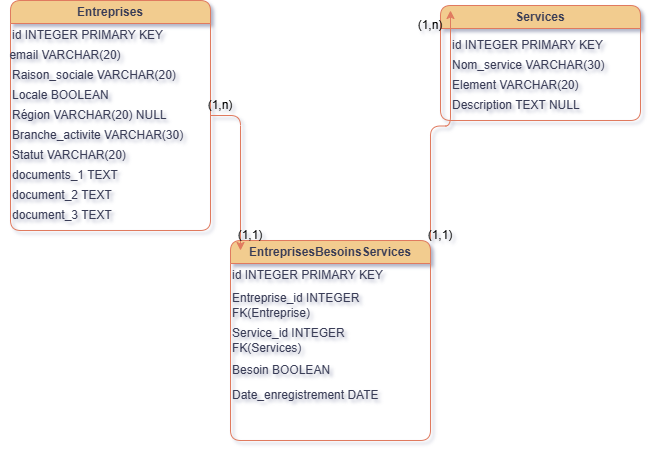
\includegraphics[width=0.8\textwidth]{model1.png}
	     \caption{Schéma de la base de données}
	     \label{fig:mcd}
	 \end{figure}

\subsection{Langages de programmation et frameworks utilisés}
Le choix de l'environnement technologique répond à des impératifs d'efficacité, de sécurité et de rapidité de déploiement. Notre choix s'est porté sur le langage \textit{Python} et le framework \textit{Django}. 

Python s'est imposé naturellement en raison de sa polyvalence et de sa suprématie dans le domaine de la Data Science, facilitant ainsi l'intégration future de nos algorithmes de mise en relation. 

Le framework de haut niveau \textit{Django}, initialement développé en 2003 pour la gestion de sites d'actualités par le journal américain \textit{Lawrence Journal-World}, est aujourd'hui une référence mondiale pour le développement d'applications web robustes. Django se distingue par son architecture orientée \textit{MTV} (Modèle-Template-Vue), qui est une déclinaison directe du traditionnel pattern \textit{MVC} (Modèle-Vue-Contrôleur) :
\begin{itemize}
	\item \textbf{Le Modèle (Model) :} Correspond à la couche de données. Il encapsule la structure de la base de données via un ORM (\textit{Object-Relational Mapping}) et gère la logique métier.
	\item \textbf{Le Template (Template) :} Gère la couche de présentation (l'interface utilisateur HTML/CSS). Il équivaut à la \textit{Vue} dans le modèle MVC classique.
	\item \textbf{La Vue (View) :} Contient la logique de contrôle. Elle intercepte les requêtes HTTP, interagit avec les Modèles pour récupérer ou modifier les données, et sélectionne le Template approprié à afficher. Elle fait office de \textit{Contrôleur}.
\end{itemize}
	
	\section*{Conclusion}
	En conclusion, la méthodologie déployée dans ce travail répond aux exigences techniques de notre double objectif. D'une part, la cartographie des besoins des entreprises s'est appuyée sur un ensemble d'outils statistiques allant des analyses descriptives (univariée et bivariée) aux méthodes multidimensionnelles, notamment l'Analyse des Correspondances Multiples (\gls{acm}), l'Analyse Factorielle Discriminante (\gls{afd}) et la Classification Ascendante Hiérarchique (\gls{cah}). D'autre part, le développement de la plateforme numérique «~Business Partnership~» repose sur une modélisation dimensionnelle de la base de données afin de garantir l'efficacité des requêtes.
	%============================================================
	%  CHAPITRE 4 : PRÉSENTATION DES RÉSULTATS
	%============================================================
	%=============================================================
	\chapter{Présentation des résultats}
	%=============================================================
	
	Ce chapitre présente l'ensemble des résultats obtenus dans le cadre
	de ce travail, structurés autour de deux axes complémentaires. Le
	premier axe est consacré à la présentation et à l'interprétation des
	résultats issus de l'analyse statistique des données de l'enquête
	réalisée par le \gls{minepat} sur la cartographie des besoins des
	entreprises du tissu productif local. Cette analyse s'articule en
	trois niveaux de profondeur croissante~: une analyse univariée
	décrivant la distribution des entreprises selon leurs caractéristiques
	principales, une analyse bivariée croisant ces caractéristiques avec
	les besoins exprimés et validant les associations observées par le
	test du $\chi^2$ de Pearson, et une analyse multidimensionnelle
	mobilisant l'Analyse des Correspondances Multiples (ACM), la
	Classification Ascendante Hiérarchique (CAH) et l'Analyse Factorielle
	Discriminante (AFD). Le second axe est consacré à la présentation de
	la plateforme \textit{Business Partnership}. L'ensemble de ces
	analyses ont été conduites sur un fichier contenant
	\textbf{1\,194 entreprises}, issues de l'enquête nationale du
	\gls{minepat} de 2025.
	
	%=============================================================
	\section{Résultats sur la cartographie des entreprises}
	\label{sec:resultats_carto}
	%=============================================================
	
	Cette section est consacrée à la présentation des résultats de l'analyse statistique des
	données collectées lors de l'enquête. Elle se veux etre progressive en débutant par une ~: description
	univariée, s'en suivra une analyse des associations bivariées, et enfin  l'exploration
	multidimensionnelle.
	\subsection{Qualité et préparation des données}
	
	Avant toute analyse, une phase de contr\^ole de la qualit\'e des
	donn\'ees a \'et\'e effectu\'ee. Le tableau~\ref{tab:qualite_donnees}
	pr\'esente les indicateurs cl\'es de cette phase.
	
	\begin{table}[H]
		\centering
		\caption{Indicateurs de qualit\'e et de pr\'eparation des donn\'ees}
		\label{tab:qualite_donnees}
		\renewcommand{\arraystretch}{1.4}
		\begin{tabularx}{\textwidth}{>{\raggedright\arraybackslash}X
				>{\centering\arraybackslash}p{3cm}
				>{\raggedright\arraybackslash}p{4cm}}
			\toprule
			\rowcolor{primary!15}
			\textbf{Indicateur} & \textbf{Valeur} & \textbf{Action} \\
			\midrule
			
			Observations initiales (fichier \texttt{identifications})
			& 1\,254 & --- \\
			
			\rowcolor{lightgray}
			Doublons d\'etect\'es
			& 60 & Supprim\'es \\
			
			Valeurs manquantes sur variable cl\'e (\texttt{secteur\_activite})
			& 0 & --- \\
			
			\rowcolor{lightgray}
			Valeurs manquantes sur \texttt{date\_debut\_activite}
			& 47 & Regroup\'ees en modalit\'e <<~Non renseign\'e~>> \\
			
			Variables exclues de l'analyse factorielle
			& 4 & \texttt{id}, \texttt{email},
			\texttt{telephone}, \texttt{site\_web} \\
			
			\rowcolor{lightgray}
			Cat\'egories de besoins initiales
			& 12 & Regroup\'ees en 7 cat\'egories \\
			
			Observations finales retenues
			& 1\,194 & Base finale utilis\'ee \\
			
			\bottomrule
		\end{tabularx}
	\end{table}
	%-------------------------------------------------------------
	\subsection{Résultats de l'analyse univariée}
	\label{subsec:univariee}
	%-------------------------------------------------------------
	
	L'analyse univariée a consisté à déterminer le nombre et le
	pourcentage d'entreprises présentant des modalités similaires sur
	les différentes variables retenues~: statut juridique, région
	d'implantation, taille, ancienneté et secteur d'activité principal.
	Elle constitue la première photographie descriptive du tissu productif
	camerounais couvert par l'enquête, et permet d'identifier les
	caractéristiques dominantes des entreprises interrogées avant
	d'explorer les relations entre leurs attributs et leurs besoins.
	
	\subsubsection{Répartition des entreprises par statut juridique}
	Le statut juridique est la forme revêtue par une entreprise. Il donne une indication sur la structure de l’entreprise et sur le cadre juridique dans lequel elle naît, évolue et interagit avec ses partenaires
	%(lecoindesentreprenerus.fr).
	La distribution des entreprises selon leur statut juridique révèle
	une prépondérance des Sociétés à Responsabilité Limitée (SARL), qui
	représentent 35,0\,\% des entreprises de l'échantillon. Les entreprises individuelles viennent en deuxième position avec 
	28,7\%. Ce qui pourrait traduire une difficulté pour les grandes entreprises à se constituer dans l'écosystème Camerounais.
	
	\begin{figure}[H]
		\centering
		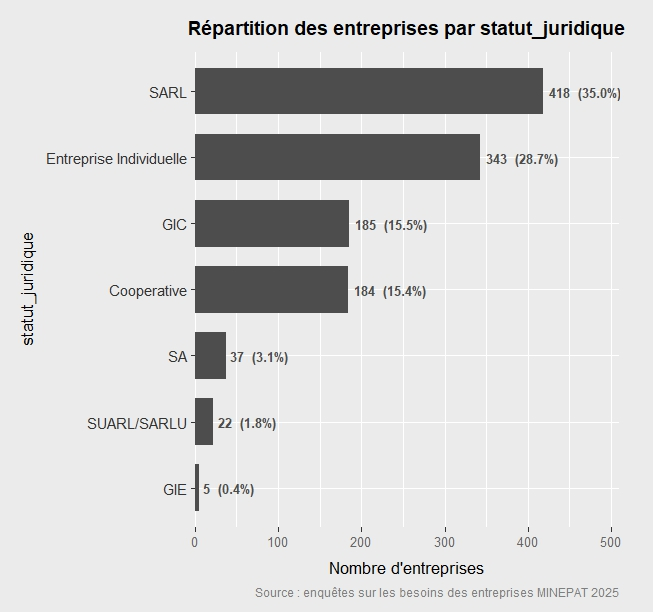
\includegraphics[width=0.75\textwidth]{statut.jpeg}
		\caption{Répartition des entreprises enquêtées par statut juridique}
		\label{fig:statut_juridique}
	\end{figure}
\newpage
	\subsubsection{Répartition des entreprises par région}
	Le Cameroun compte 10 régions et au vue des données exploitées, nous pouvons relever une répartition assez inéquitable.
	En effet plus de la moitié des entreprises interrogées sont implentées dans les régions du Centre et du Littoral avec
	respectivement un pourcentage de 39,3\% et 17,8\%. Les autres régions se partagent 42,9\% avec les régions du Nord-Ouest et du Sud-Ouest qui ferment la marque avec respectivement 2,7\% et 2,8\% des entreprises étudiées. 
	\begin{figure}[H]
		\centering
		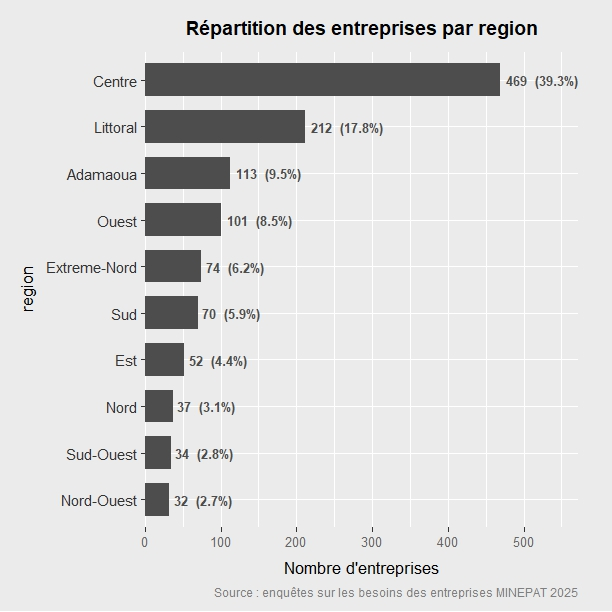
\includegraphics[width=0.75\textwidth]{repartition_region.jpeg}
		\caption{Répartition des entreprises enquêtées par région}
		\label{fig:region}
	\end{figure}
	
	
	
	\subsubsection{Répartition des entreprises par taille}
	La taille de l'entreprise repose sur le nombre de salariés et le chiffre d'affaires annuel de celle ci. %(https://blog.hubspot.fr/sales/taille-entreprise-classification)
	La discribution des entreprises par taille reflète la structure du tissus productif camerounais,
	caractérisé par une prédominance des petites entreprises et des très petites entreprises Les Grandes Entreprises sont très peu nombreuses et constituent 1,3\% des entreprises interrogées.
	\begin{figure}[H]
		\centering
		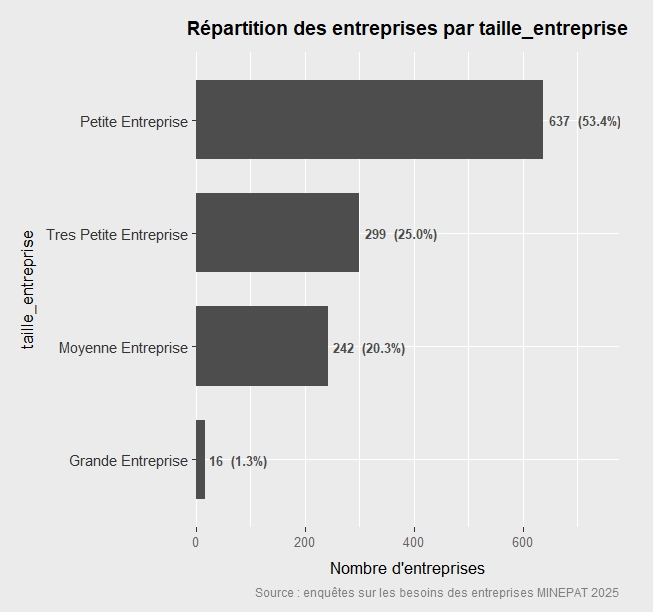
\includegraphics[width=0.75\textwidth]{repartition_taille.jpeg}
		\caption{Répartition des entreprises enquêtées par taille}
		\label{fig:taille}
	\end{figure}
	
	\subsubsection{Répartition des entreprises par ancienneté}
	La capacité d'une entreprise à se maintenir dans le temps témoigne de sa résilience et de sa force. 
	La répartition des entreprises par ancienneté indique que ce sont les entreprises de 5 à 9 ans
	d'ages qui ce sont le plus prétées au jeu avec 39,0\% de participation. Les entreprises ayant pas plus de 4  ans sont relativement nombreuses avec un pourcentage de 31,2\%. 
	\begin{figure}[H]
		\centering
		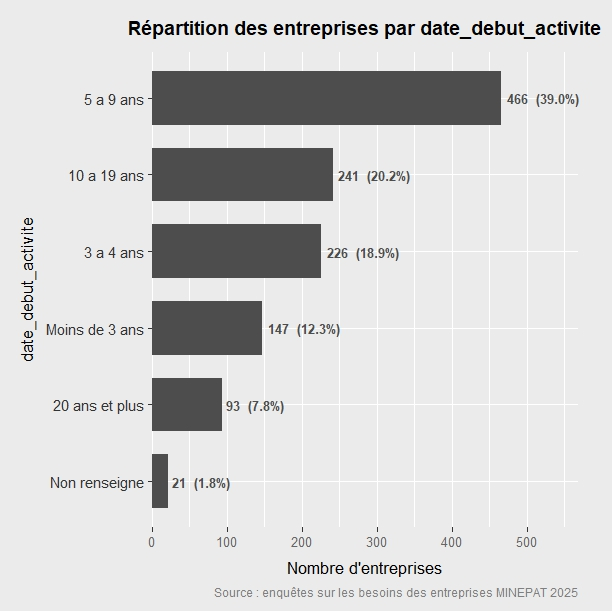
\includegraphics[width=0.75\textwidth]{anciennete.jpeg}
		\caption{Répartition des entreprises enquêtées par ancienneté}
		\label{fig:anciennete}
	\end{figure}
	
	
	\subsubsection{Répartition des entreprises par secteur d'activité}
	Les secteurs d'activités des entreprises locales sont plutot diversifiés. Nous avons pu relever que 
le secteur de l'agriculture et de l'agroalimentaire est le plus représenté dans les entreprises locales, 
il détient à lui seul 62,6\% des entreprises étudiées. Les secteurs de l'industrie manufacturière et des 
Technologies de l'Informations et de la Communication sont assez peu nombreuses avec respectivement des taux de 5,2 \% et 3,7 \%. 
	\begin{figure}[H]
		\centering
		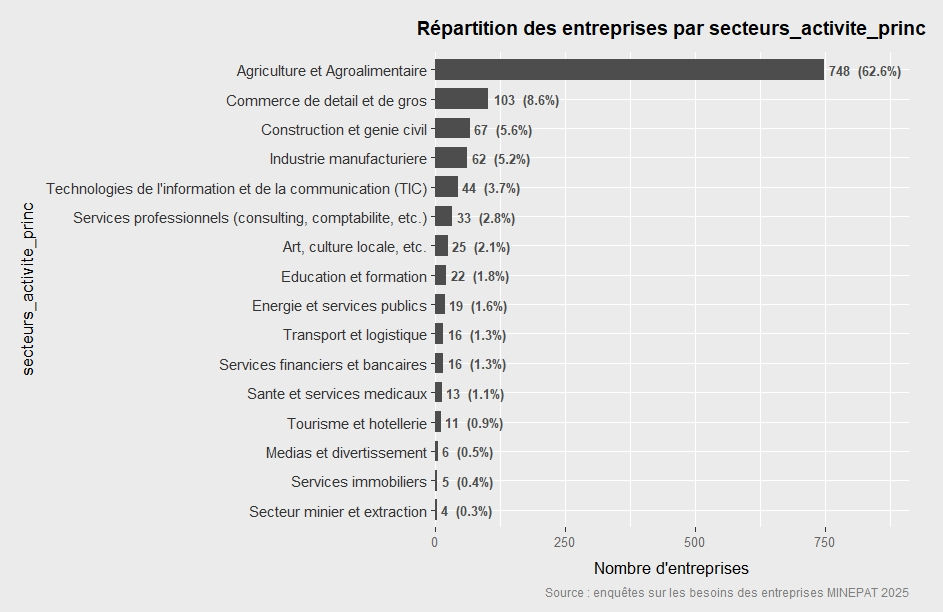
\includegraphics[width=0.75\textwidth]{repartition_activite.jpeg}
		\caption{Répartition des entreprises enquêtées par secteur d'activité}
		\label{fig:secteur}
	\end{figure}

	\subsubsection{Répartition des besoins exprimés}
	
	Les entreprises interrogées ont exprimé des besoins divers en relation avec les problèmes rencontrés quotidiennement. Le besoin qui revient le plus est celui du financement avec un taux de 96,2\% ce qui pourrait s'expliquer par une prédominance des TPE et des PME qui ont besoin de fonds pour une meilleur implentation. Vient ensuite le besoin en équipements avec 93,0\%, le besoin de transport est la moins fréquente ce qui traduirait l'existence d'infrastructures adéquat pour l'acheminement des produits.
	\begin{figure}[H]
		\centering
		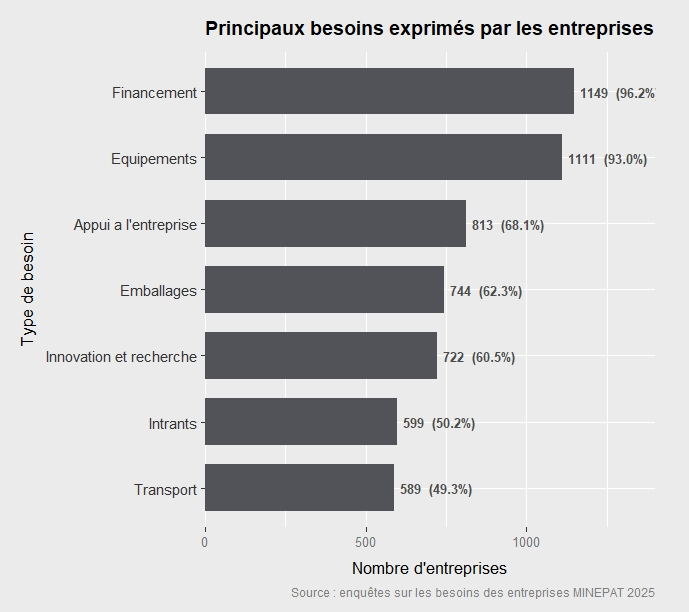
\includegraphics[width=0.75\textwidth]{besoinsCorriges.jpeg}
		\caption{Répartition globale des besoins exprimés par les entreprises
			enquêtées}
		\label{fig:besoins_global}
		\end{figure}
			
			%-------------------------------------------------------------
			\subsection{Résultats de l'analyse bivariée}
			\label{subsec:bivariee}
			%-------------------------------------------------------------
			
			L'analyse bivariée a consisté à croiser les variables descriptives
			des entreprises avec les besoins qu'elles ont exprimés, afin
			d'identifier d'éventuelles associations structurelles entre les
			caractéristiques des entreprises et leurs besoins spécifiques. Deux
			outils ont été mobilisés~: les tableaux de contingence, qui permettent
			de visualiser la distribution conjointe des variables, et le test du
			$\chi^2$ de Pearson accompagné du coefficient $V$ de Cramér, qui
			permettent de tester et de quantifier l'intensité de ces associations
			\cite{saporta_2010}.
			
			\subsubsection{Répartition des besoins selon le statut juridique}
			
			Les figures ci-dessous présentent la distribution des besoins des
			entreprises selon leur statut juridique, ainsi que les résultats du
			test d'association correspondant.
			
			\begin{figure}[H]
				\centering
				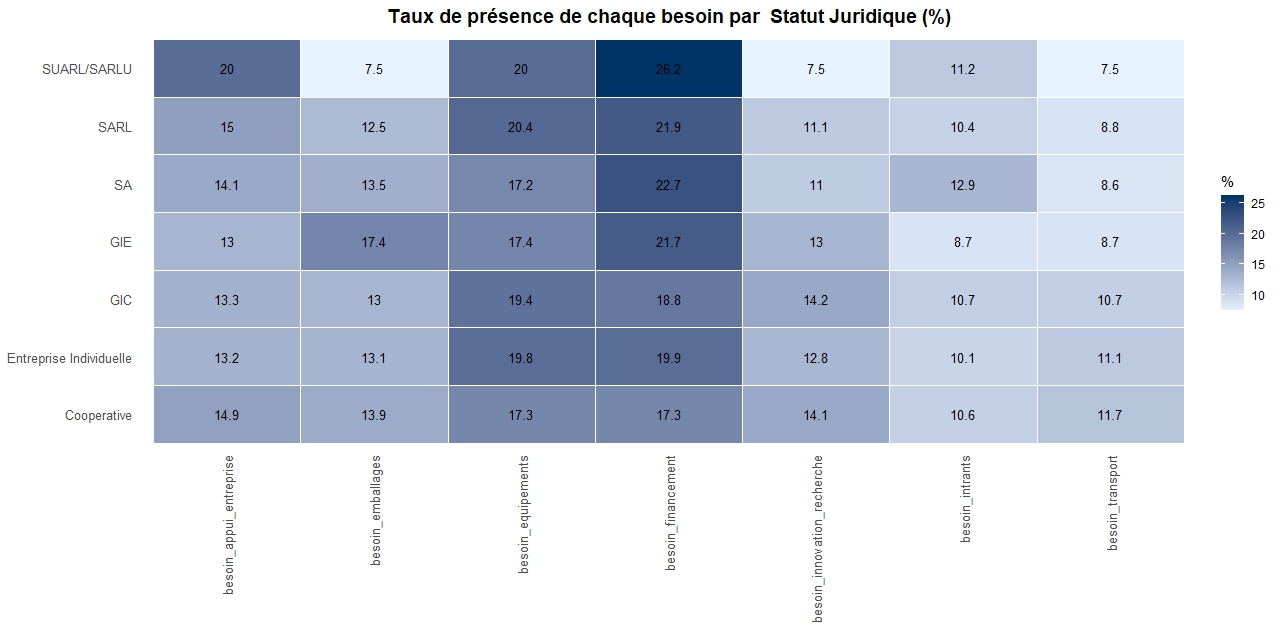
\includegraphics[width=\textwidth]{carte_chaleur_besoins_statut_juridique.jpeg}
				\caption{Distribution des besoins des entreprises selon le statut
					juridique}
				\label{fig:besoins_statut}
			\end{figure}
			
			\begin{table}[H]
				\centering
				\caption{Test du $\chi^2$ entre le statut juridique et les besoins
					des entreprises}
				\label{tab:khi2_statut}
				\renewcommand{\arraystretch}{1.4}
				\begin{tabularx}{\textwidth}{>{\raggedright\arraybackslash}X
						r r
						>{\centering\arraybackslash}p{2.8cm}
						r}
					\toprule
					\rowcolor{primary!15}
					\textbf{Besoin} & \textbf{$\chi^2$} & \textbf{p-valeur}
					& \textbf{Significatif} & \textbf{$V$ Cramér} \\
					\midrule
					Besoin en intrants        & 14,26 & 0,027  & Oui ($p < 0{,}05$) & 0,109 \\
					\rowcolor{lightgray}
					Besoin en financement     &  2,94 & 0,817  & Non                & 0,050 \\
					Besoin en emballages      & 44,47 & $<0{,}001$ & Oui ($p < 0{,}05$) & 0,193 \\
					\rowcolor{lightgray}
					Besoin en transport       & 50,44 & $<0{,}001$ & Oui ($p < 0{,}05$) & 0,206 \\
					Appui aux entreprises     & 26,32 & $<0{,}001$ & Oui ($p < 0{,}05$) & 0,148 \\
					\rowcolor{lightgray}
					Besoin en équipements     & 61,66 & $<0{,}001$ & Oui ($p < 0{,}05$) & 0,227 \\
					Innovation et recherche   & 77,88 & $<0{,}001$ & Oui ($p < 0{,}05$) & 0,255 \\
					\bottomrule
				\end{tabularx}
			\end{table}
			
			Les résultats du test du $\chi^2$ révèlent que le statut juridique
			est significativement associé à six des sept besoins étudiés, à
			l'exception du besoin en financement ($\chi^2 = 2{,}94$~;
			$p = 0{,}817$). Les associations les plus fortes concernent le besoin
			en innovation et en recherche ($V = 0{,}255$) et le besoin en
			équipements ($V = 0{,}227$), suggérant que la nature juridique de
			l'entreprise influence significativement la manière dont elle exprime
			ses besoins technologiques. Les entreprises de type SUARL/SARLU
			présentent notamment le taux le plus élevé de besoin en appui aux
			entreprises (20,0\,\%) et en financement (26,2\,\%), tandis que les
			Coopératives expriment davantage de besoins en innovation
			(14,1\,\%). Le besoin en financement constitue une exception notable~:
			il est exprimé de manière relativement homogène quelle que soit la
			forme juridique de l'entreprise, ce qui suggère que la contrainte
			financière est une réalité transversale à l'ensemble du tissu
			économique, indépendante du cadre juridique de l'entreprise.
			
			\subsubsection{Répartition des besoins selon la région}
			
			\begin{figure}[H]
				\centering
				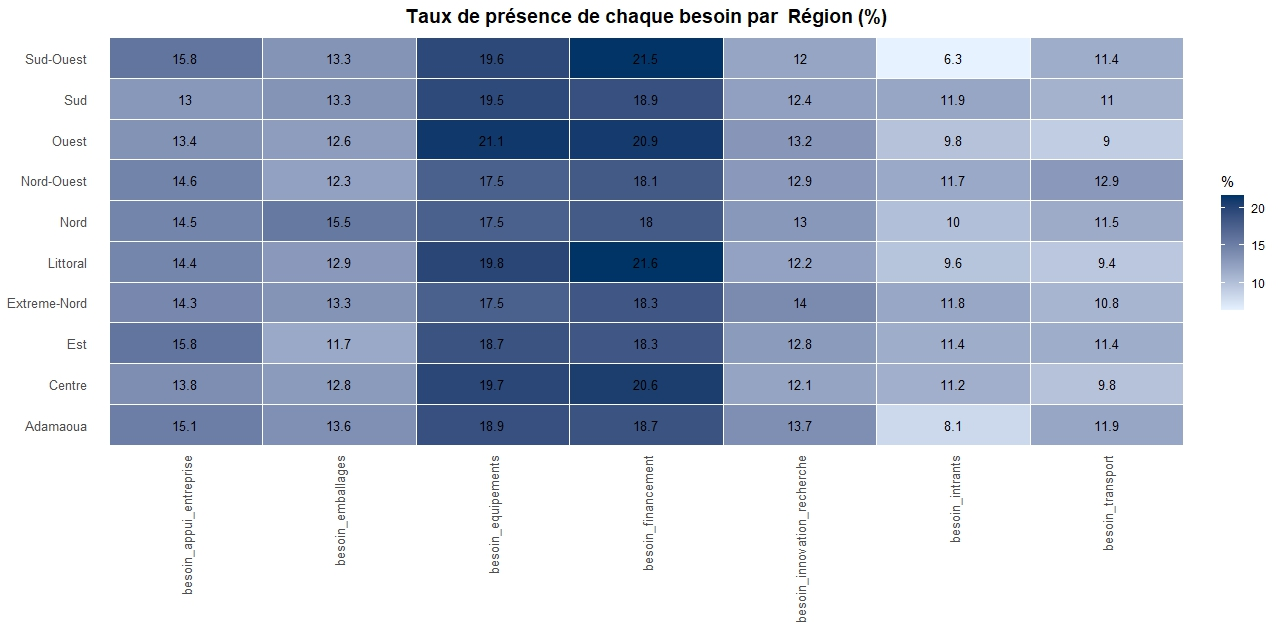
\includegraphics[width=\textwidth]{carte_chaleur_besoins_region.jpeg}
				\caption{Distribution des besoins des entreprises selon la région
					d'implantation}
				\label{fig:besoins_region}
			\end{figure}
			
			\begin{table}[H]
				\centering
				\caption{Test du $\chi^2$ entre la région d'implantation et les besoins
					des entreprises}
				\label{tab:khi2_region}
				\renewcommand{\arraystretch}{1.4}
				\begin{tabularx}{\textwidth}{>{\raggedright\arraybackslash}X
						r r
						>{\centering\arraybackslash}p{2.8cm}
						r}
					\toprule
					\rowcolor{primary!15}
					\textbf{Besoin} & \textbf{$\chi^2$} & \textbf{p-valeur}
					& \textbf{Significatif} & \textbf{$V$ Cramér} \\
					\midrule
					Besoin en intrants        & 28,91 & $<0{,}001$ & Oui ($p < 0{,}05$) & 0,156 \\
					\rowcolor{lightgray}
					Besoin en financement     &  6,21 & 0,718  & Non                    & 0,072 \\
					Besoin en emballages      & 18,69 & 0,028  & Oui ($p < 0{,}05$)    & 0,125 \\
					\rowcolor{lightgray}
					Besoin en transport       & 29,83 & $<0{,}001$ & Oui ($p < 0{,}05$) & 0,158 \\
					Appui aux entreprises     & 23,36 & 0,005  & Oui ($p < 0{,}05$)    & 0,140 \\
					\rowcolor{lightgray}
					Besoin en équipements     & 28,25 & $<0{,}001$ & Oui ($p < 0{,}05$) & 0,154 \\
					Innovation et recherche   & 23,77 & 0,005  & Oui ($p < 0{,}05$)    & 0,141 \\
					\bottomrule
				\end{tabularx}
			\end{table}
			
			La région d'implantation s'avère significativement associée à six
			besoins sur sept, le besoin en financement étant à nouveau le seul
			pour lequel aucune association significative n'est détectée
			($\chi^2 = 6{,}21$~; $p = 0{,}718$). Ce résultat confirme le
			caractère transversal de la contrainte financière, commune à
			l'ensemble des régions. Les besoins en transport ($V = 0{,}158$)
			et en intrants ($V = 0{,}156$) présentent les associations les plus
			fortes avec la région, ce qui est cohérent avec les disparités
			infrastructurelles importantes entre les régions camerounaises.
			Les régions du Nord-Ouest de l'Adamaoua et de l'Est, qui concentrent une part
			significative des entreprises à besoins en transport élevés,
			illustrent comment les contraintes géographiques et l'état des
			infrastructures conditionnent les priorités des entreprises locales.
			
			\subsubsection{Répartition des besoins selon l'ancienneté}
			
			\begin{figure}[H]
				\centering
				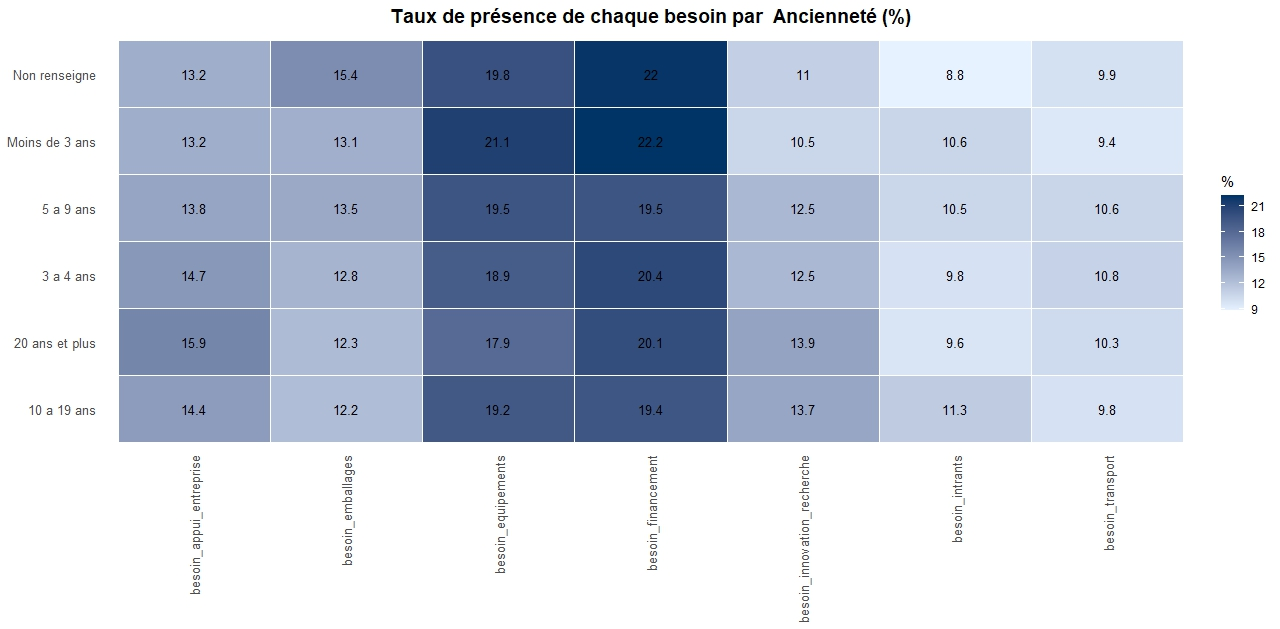
\includegraphics[width=\textwidth]{carte_chaleur_besoins_anciennete.jpeg}
				\caption{Distribution des besoins des entreprises selon leur
					ancienneté}
				\label{fig:besoins_anciennete}
			\end{figure}
			
			\begin{table}[H]
				\centering
				\caption{Test du $\chi^2$ entre l'ancienneté et les besoins
					des entreprises}
				\label{tab:khi2_anciennete}
				\renewcommand{\arraystretch}{1.4}
				\begin{tabularx}{\textwidth}{>{\raggedright\arraybackslash}X
						r r
						>{\centering\arraybackslash}p{2.8cm}
						r}
					\toprule
					\rowcolor{primary!15}
					\textbf{Besoin} & \textbf{$\chi^2$} & \textbf{p-valeur}
					& \textbf{Significatif} & \textbf{$V$ Cramér} \\
					\midrule
					Besoin en intrants        &  6,46 & 0,264  & Non                 & 0,074 \\
					\rowcolor{lightgray}
					Besoin en financement     &  4,44 & 0,488  & Non                 & 0,061 \\
					Besoin en emballages      &  5,09 & 0,405  & Non                 & 0,065 \\
					\rowcolor{lightgray}
					Besoin en transport       &  5,52 & 0,356  & Non                 & 0,068 \\
					Appui aux entreprises     & 11,84 & 0,037  & Oui ($p < 0{,}05$)  & 0,100 \\
					\rowcolor{lightgray}
					Besoin en équipements     & 14,84 & 0,011  & Oui ($p < 0{,}05$)  & 0,111 \\
					Innovation et recherche   & 20,10 & 0,001  & Oui ($p < 0{,}05$)  & 0,130 \\
					\bottomrule
				\end{tabularx}
			\end{table}
			
			L'ancienneté de l'entreprise est le critère présentant le moins
			d'associations significatives avec les besoins, puisque seulement
			trois besoins sur sept lui sont significativement liés. Les entreprises
			jeunes (moins de 3 ans) expriment davantage de besoins en financement
			(22,2\,\%) et en équipements (21,1\,\%), ce qui s'explique par leur
			stade de développement~: en phase de démarrage, l'accès aux
			ressources matérielles et financières constitue la contrainte
			prioritaire. À l'inverse, les entreprises plus matures (20 ans et
			plus) expriment un besoin en innovation et en recherche plus marqué
			(13,9\,\%), témoignant d'une préoccupation croissante pour la
			compétitivité à long terme et la modernisation technologique au fur
			et à mesure que l'entreprise se consolide.
			
			\subsubsection{Répartition des besoins selon le secteur d'activité}
			
			\begin{figure}[H]
				\centering
				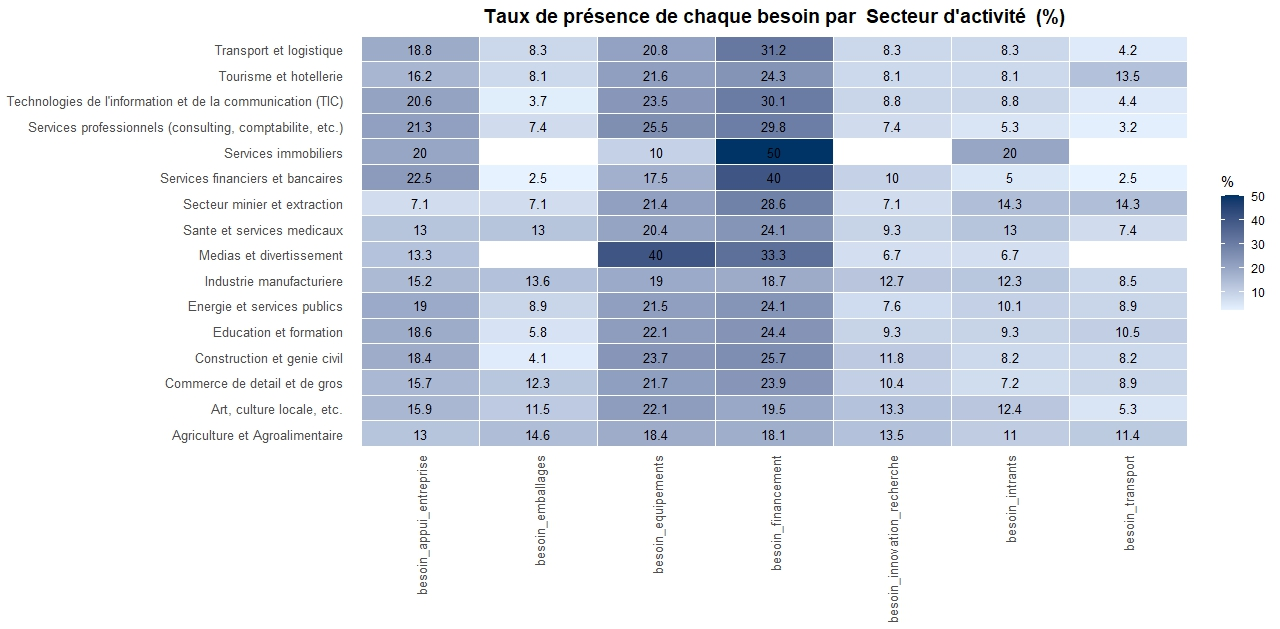
\includegraphics[width=\textwidth]{carte_chaleur_besoins_secteurs_activite.jpeg}
				\caption{Distribution des besoins des entreprises selon le secteur
					d'activité}
				\label{fig:besoins_secteur}
			\end{figure}
			
			\begin{table}[H]
				\centering
				\caption{Test du $\chi^2$ entre le secteur d'activité et les besoins
					des entreprises}
				\label{tab:khi2_secteur}
				\renewcommand{\arraystretch}{1.4}
				\begin{tabularx}{\textwidth}{>{\raggedright\arraybackslash}X
						r r
						>{\centering\arraybackslash}p{2.8cm}
						r}
					\toprule
					\rowcolor{primary!15}
					\textbf{Besoin} & \textbf{$\chi^2$} & \textbf{p-valeur}
					& \textbf{Significatif} & \textbf{$V$ Cramér} \\
					\midrule
					Besoin en intrants        & 103,48 & $<0{,}001$ & Oui ($p < 0{,}05$) & 0,294 \\
					\rowcolor{lightgray}
					Besoin en financement     &  34,10 & 0,003  & Oui ($p < 0{,}05$)    & 0,169 \\
					Besoin en emballages      & 306,81 & $<0{,}001$ & Oui ($p < 0{,}05$) & 0,507 \\
					\rowcolor{lightgray}
					Besoin en transport       & 147,87 & $<0{,}001$ & Oui ($p < 0{,}05$) & 0,352 \\
					Appui aux entreprises     &  20,13 & 0,167  & Non                    & 0,130 \\
					\rowcolor{lightgray}
					Besoin en équipements     & 239,10 & $<0{,}001$ & Oui ($p < 0{,}05$) & 0,447 \\
					Innovation et recherche   & 163,49 & $<0{,}001$ & Oui ($p < 0{,}05$) & 0,370 \\
					\bottomrule
				\end{tabularx}
			\end{table}
			
			Le secteur d'activité constitue la variable présentant les
			associations les plus fortes avec les besoins des entreprises~:
			six besoins sur sept lui sont significativement liés, avec des
			valeurs de $V$ de Cramér particulièrement élevées, notamment pour
			le besoin en emballages ($V = 0{,}507$), le besoin en équipements
			($V = 0{,}447$) et le besoin en transport ($V = 0{,}352$). Ces
			résultats confirment l'intuition selon laquelle le secteur d'activité
			est le principal déterminant de la nature des besoins exprimés par
			les entreprises. Les entreprises du secteur des Services immobiliers
			expriment le taux de besoin en financement le plus élevé (50,0\,\%),
			tandis que les entreprises du secteur des Médias et Divertissement
			présentent un besoin en équipements particulièrement fort (40,0\,\%).
			Le besoin en appui aux entreprises est le seul besoin pour lequel
			aucune association significative avec le secteur d'activité n'est
			détectée ($p = 0{,}167$), confirmant son caractère transversal à
			l'ensemble des secteurs.
			\subsubsection{Répartition des besoins selon la taille de l'entreprise}
			
			\begin{figure}[H]
				\centering
				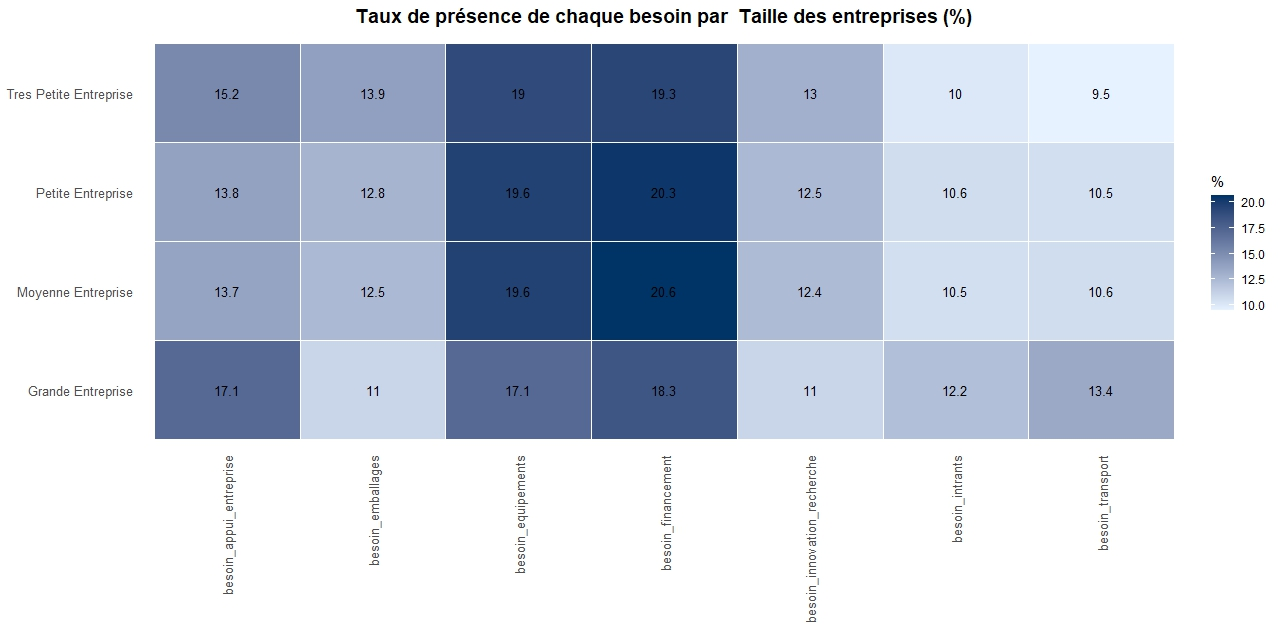
\includegraphics[width=\textwidth]{carte_chaleur_besoins_taille_entreprise.jpeg}
				\caption{Distribution des besoins des entreprises selon leur taille}
				\label{fig:besoins_taille}
			\end{figure}
			
			\begin{table}[H]
				\centering
				\caption{Test du $\chi^2$ entre la taille de l'entreprise et ses besoins}
				\label{tab:khi2_taille}
				\renewcommand{\arraystretch}{1.4}
				\begin{tabularx}{\textwidth}{>{\raggedright\arraybackslash}X
						r r
						>{\centering\arraybackslash}p{3cm}
						r}
					\toprule
					\rowcolor{primary!15}
					\textbf{Besoin} & \textbf{$\chi^2$} & \textbf{p-valeur}
					& \textbf{Significatif} & \textbf{$V$ Cramér} \\
					\midrule
					
					Besoin en intrants
					& 1,01 & 0,799 & Non & 0,029 \\
					
					\rowcolor{lightgray}
					Besoin en financement
					& 5,67 & 0,129 & Non & 0,069 \\
					
					Besoin en emballages
					& 7,48 & 0,058 & Non & 0,079 \\
					
					\rowcolor{lightgray}
					Besoin en transport
					& 3,20 & 0,362 & Non & 0,052 \\
					
					Besoin en appui aux entreprises
					& 13,95 & 0,003 & Oui ($p < 0{,}05$) & 0,108 \\
					
					\rowcolor{lightgray}
					Besoin en équipements
					& 2,25 & 0,521 & Non & 0,043 \\
					
					Innovation et recherche
					& 2,85 & 0,415 & Non & 0,049 \\
					
					\bottomrule
				\end{tabularx}
			\end{table}
			
			Les résultats du test du $\chi^2$ révèlent que la taille de
			l'entreprise n'est significativement associée qu'à un seul besoin sur
			les sept étudiés~: le besoin en appui aux entreprises ($\chi^2 =
			13{,}95$~; $p = 0{,}003$~; $V = 0{,}108$). Ce résultat est
			interprétable de manière intuitive~: les besoins d'accompagnement et
			d'appui institutionnel sont davantage ressentis par les petites
			structures, qui ne disposent pas en interne des ressources humaines
			et organisationnelles nécessaires pour gérer leurs activités de
			manière autonome, contrairement aux grandes entreprises qui
			internalisent généralement ces fonctions. L'association reste
			néanmoins modérée ($V = 0{,}108$), ce qui suggère que d'autres
			facteurs que la taille influencent également ce besoin.
			
			Pour les six autres besoins étudiés, aucune association
			statistiquement significative avec la taille de l'entreprise n'est
			détectée. Ce constat est particulièrement notable pour le besoin en
			financement ($\chi^2 = 5{,}67$~; $p = 0{,}129$), qui se confirme une
			nouvelle fois comme une contrainte universelle, indépendante de la
			taille de l'entreprise. De même, le besoin en équipements ($p =
			0{,}521$) et le besoin en innovation ($p = 0{,}415$) ne sont pas
			significativement liés à la taille, ce qui peut paraître surprenant
			mais s'explique par le fait que les besoins technologiques concernent
			l'ensemble des entreprises quel que soit leur niveau de développement,
			même si leur nature précise peut différer.
			
			
			
			
			%-------------------------------------------------------------
			\subsection{Résultats de l'analyse multidimensionnelle}
			\label{subsec:multi}
			%-------------------------------------------------------------
			
			Les analyses univariée et bivariée ont permis de décrire le tissu
			économique et d'identifier des associations entre les caractéristiques
			des entreprises et leurs besoins. Cependant, ces méthodes ne
			permettent pas d'appréhender simultanément l'ensemble des relations
			entre les variables dans leur globalité. L'analyse multidimensionnelle
			vient combler cette limite en offrant une représentation synthétique
			des données dans un espace factoriel de dimension réduite, à partir
			duquel des groupes d'entreprises aux profils similaires peuvent être
			construits et caractérisés. Elle s'articule en trois étapes
			successives~: l'ACM pour la réduction de dimension, la CAH pour
			la construction des classes, et l'AFD pour leur validation et
			caractérisation.
			
			\subsubsection{Analyse des Correspondances Multiples (ACM)}
			
			L'ACM a été conduite à l'aide du package \texttt{FactoMineR} du
			langage R %\cite{lebart_morineau_piron_1995}
			, sur l'ensemble des
			variables qualitatives retenues pour décrire les entreprises et
			leurs besoins. Son objectif principal est d'identifier les axes
			factoriels sur lesquels les données présentent la plus grande
			variabilité, afin de produire une représentation synthétique du
			nuage d'entreprises dans un espace de dimension réduit.
			
			\paragraph{Valeurs propres et inertie expliquée}
			
			Le choix du nombre d'axes à retenir s'effectue à partir de
			l'examen de l'éboulis des valeurs propres, qui représente la
			part d'inertie totale expliquée par chacun des axes factoriels.
			
			\begin{figure}[H]
				\centering
				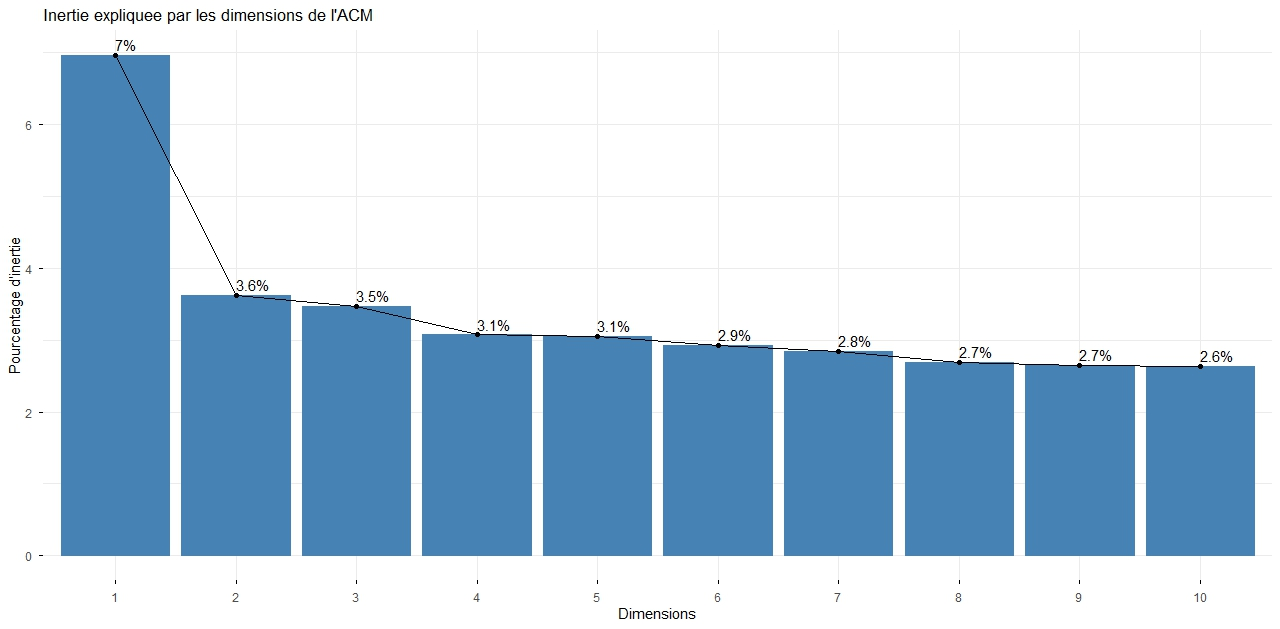
\includegraphics[width=0.75\textwidth]{contributionValeursPropres.jpeg}
				\caption{Éboulis des valeurs propres de l'ACM --- part d'inertie
					expliquée par axe factoriel}
				\label{fig:acm_vp}
			\end{figure}
			
			L’objectif principal de l’ACM étant l’interprétation à partir des projections des modalités sur les axes factoriels, le nombre d’axes à retenir est choisi en utilisant le critère du pourcentage d'inertie expliqué par les axes factorielles. Il est souvent conseillé de sélectionner les axes factorielles qui expliquent au moins 80\% de l'inertie total du nuage dans notre cas, nous avons retenu les 5 premiers axes factoriels qui avec les valeurs propres corrigées expliquent 88,74\% de l'inertie totale.
			
			
			\paragraph{Projection des modalités sur le premier plan factoriel}
		

			La projection des modalités sur les deux premiers axes factoriels
			permet de visualiser les associations entre les différentes modalités
			des variables et d'identifier les oppositions structurantes du nuage
			de points.
			
			\begin{figure}[H]
				\centering
				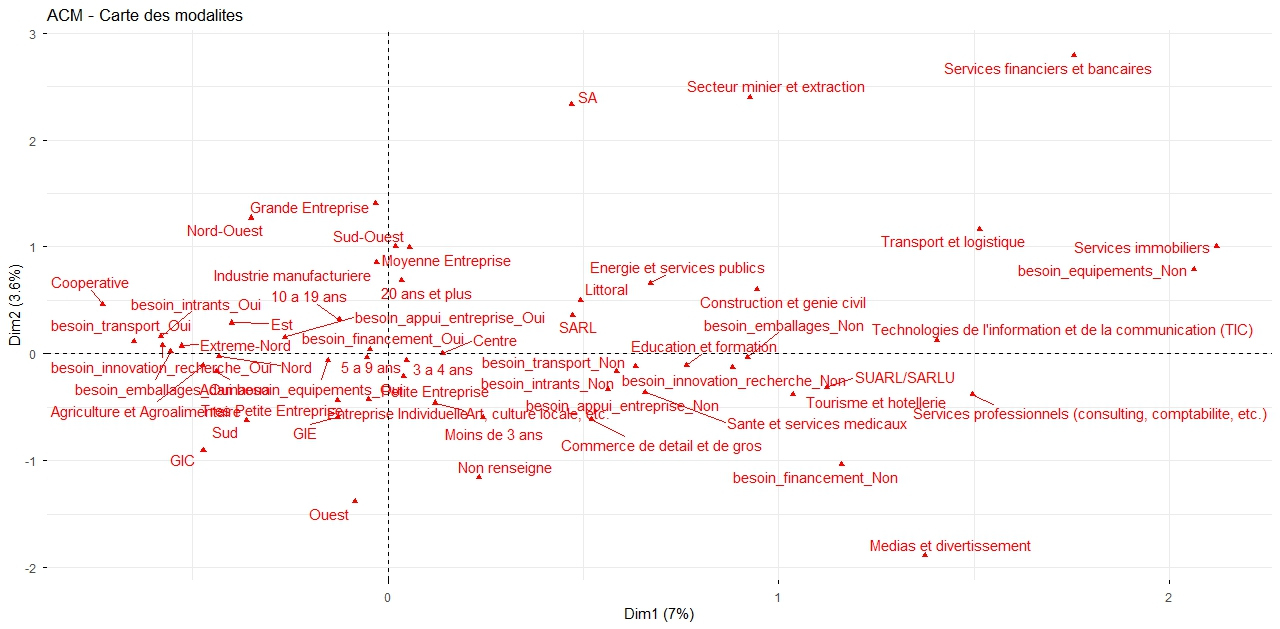
\includegraphics[width=\textwidth]{projectionDesCategories.jpeg}
				\caption{Projection des modalités sur le premier plan factoriel
					de l'ACM (axes 1 et 2)}
				\label{fig:acm_projection}
			\end{figure}
			
			On observe dans la figure \ref{fig:acm_projection} que bien de modalités sont assez proches des deux premiers axes factoriels. L'axe 1 oppose les entreprises tertiaires des entreprises du secteur primaire à travers la présence ou non d'un certains nombre de besoins et la répartition des secteurs d'activités. L'axe 2 permet de discriminer les statuts des entreprises et leurs tailles. On peut remarquer la présence quasi au centre du besoin en financement considéré comme un besoin transversal des entreprises.
			
			\paragraph{Variables contribuant aux axes factoriels}
			
			Les figures suivantes présentent les contributions des variables
			au premier et au second axe factoriel, permettant d'identifier
			les attributs les plus structurants de chaque dimension.
			
			\begin{figure}[H]
				\centering
				\begin{minipage}{0.48\textwidth}
					\centering
					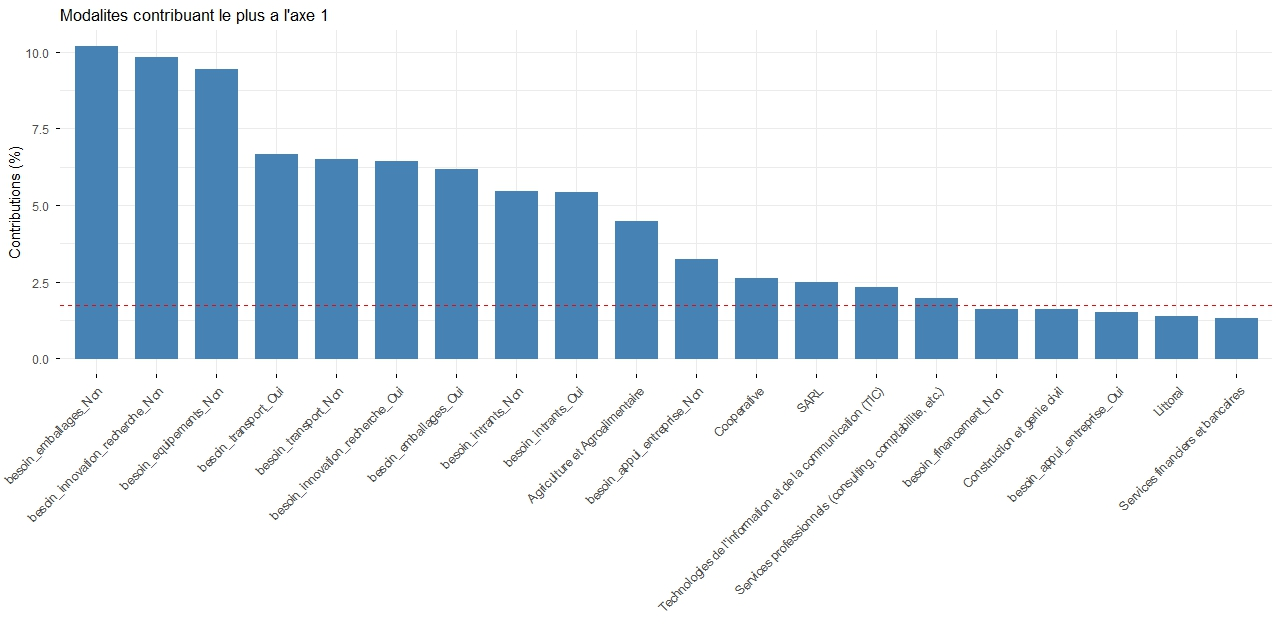
\includegraphics[width=\textwidth]{contributionCategoriesAlAxe1.jpeg}
					\caption{Contributions des modalités au premier axe factoriel}
					\label{fig:acm_contrib1}
				\end{minipage}
				\hfill
				\begin{minipage}{0.48\textwidth}
					\centering
					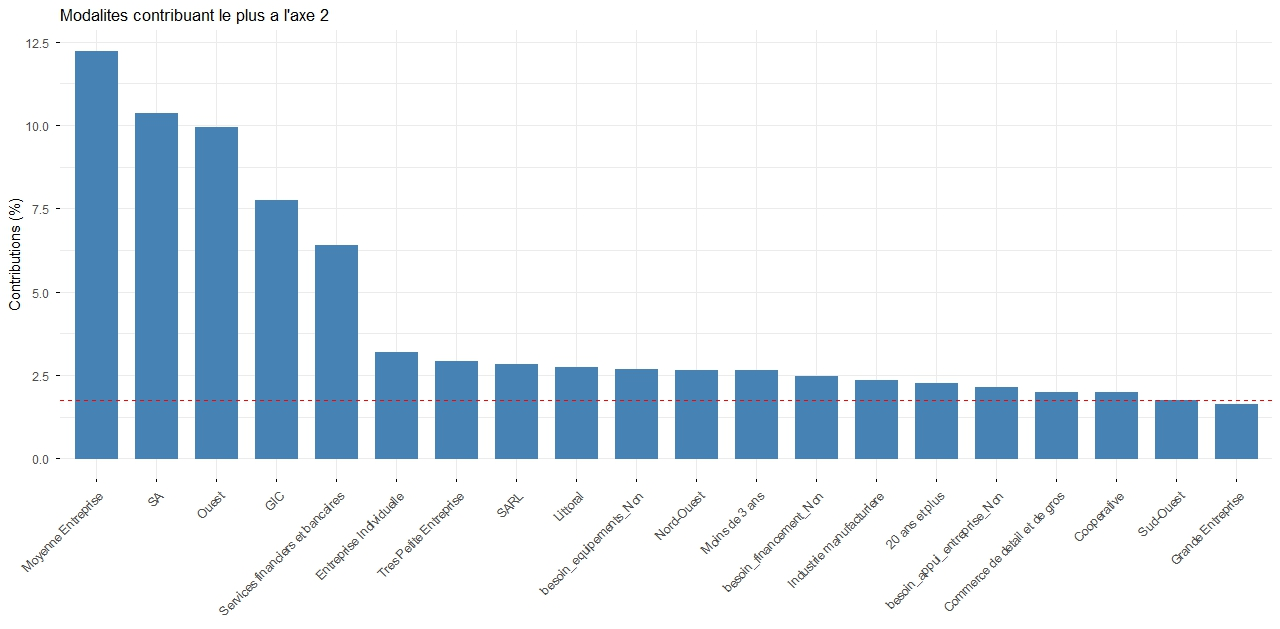
\includegraphics[width=\textwidth]{contributionCategorieALAxe2.jpeg}
					\caption{Contributions des modalités au second axe factoriel}
					\label{fig:acm_contrib2}
				\end{minipage}
			\end{figure}
			
		Le premier axe factoriel (Dim 1), qui capte la plus grande part de
		l'inertie de la structure des données (7\,\%), est fortement construit
		par des variables liées aux besoins opérationnels et techniques des
		structures. En observant l'éboulis des contributions, un groupe de
		trois modalités se détache très nettement au-dessus des autres,
		frôlant les 10\,\% de contribution chacune~:
		\texttt{besoin\_emballages\_Non},
		\texttt{besoin\_innovation\_recherche\_Non} et
		\texttt{besoin\_equipements\_Non}.
		Viennent ensuite, de manière équilibrée (entre 5\,\% et 7\,\%),
		les expressions contrastées des besoins logistiques et techniques
		(\texttt{besoin\_transport\_Oui},
		\texttt{besoin\_transport\_Non},
		\texttt{besoin\_innovation\_recherche\_Oui},
		\texttt{besoin\_emballages\_Oui}).
		Le seuil de contribution moyenne (ligne pointillée rouge à environ
		1{,}8\,\%) met en évidence que l'Axe~1 est presque exclusivement
		dicté par la dichotomie entre la présence et l'absence de besoins
		matériels et d'innovation au sein des structures.

		
		Le second axe factoriel (Dim 2, 3.6 \% de l'inertie) est quant à lui défini par des variables purement statutaires, institutionnelles et géographiques, marquant une rupture totale avec la logique de besoins de l'axe précédent. Le graphique des contributions montre que la construction de cet axe repose majoritairement sur cinq piliers qui dépassent de loin le seuil de contribution théorique : la taille moyenne d'entreprise (Moyenne Entreprise, ~12 \%), la forme juridique de Société Anonyme (SA, ~10.5 \%), la région de l'Ouest (~10 \%), le statut de Groupement d'Intérêt Communautaire (GIC, ~7.5 \%) et le secteur des Services financiers et bancaires (~6.5 \%). Les variables d'âge de l'entreprise ou de besoins opérationnels n'exercent ici qu'une influence très secondaire, ce qui confirme que l'Axe 2 capte spécifiquement le niveau de formalisation et de structuration légale des entités.
			
			\subsubsection{Classification Ascendante Hiérarchique (CAH)}
			
			La CAH a été conduite à partir des coordonnées factorielles des
			entreprises sur les axes retenus lors de l'ACM, en utilisant la
			méthode d'agrégation de Ward qui minimise la perte d'inertie
			inter-classes à chaque étape de fusion \cite{saporta_2010}.
			
			\paragraph{Dendrogramme et choix du nombre de classes}
			
			Le dendrogramme obtenu à l'issue de la CAH permet de visualiser
			la hiérarchie des regroupements.
			
			\begin{figure}[H]
				\centering
				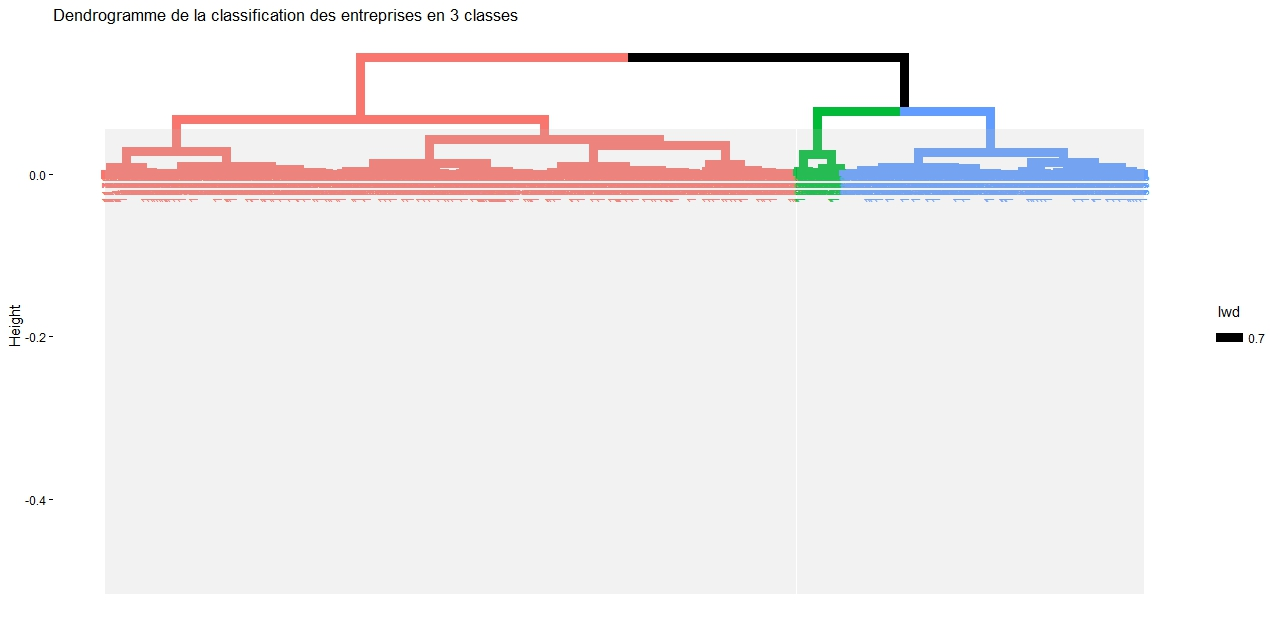
\includegraphics[width=0.85\textwidth]{dendrogramme.jpeg}
				\caption{Dendrogramme de la Classification Ascendante Hiérarchique
					(méthode de Ward)}
				\label{fig:dendrogramme}
			\end{figure}
			
		Nous avons choisi de partitionner le jeu de données en trois classes. Du fait qu'un nombre trop élevé de classe pourrait très mal représenter les groupes du jeu de donnée et un nombre trop petit traduirait une difficulté pour distinguer les groupes.
			
			\paragraph{Visualisation de la partition obtenue}
			
			\begin{figure}[H]
				\centering
				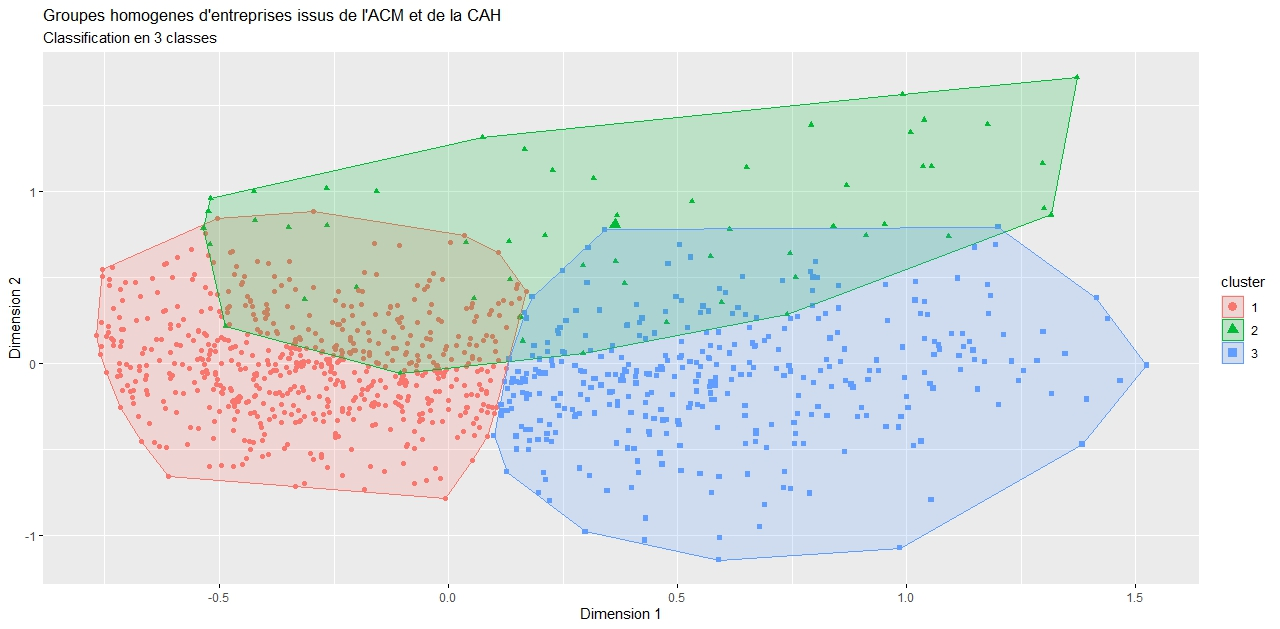
\includegraphics[width=\textwidth]{CAH.jpeg}
				\caption{Projection des trois classes obtenues par CAH sur le
					premier plan factoriel de l'ACM}
				\label{fig:cah_classes}
			\end{figure}
			
			La figure~\ref{fig:cah_classes} représente les trois classes
			d'entreprises obtenues, projetées sur le premier plan factoriel
			de l'ACM. La séparation visuelle des classes dans cet espace
			factoriel confirme la cohérence de la partition obtenue~: les
			trois groupes occupent des zones distinctes du plan factoriel,
			témoignant d'une bonne homogénéité intra-classe et d'une
			séparation satisfaisante inter-classes.
		
			\begin{itemize}
				\item \textbf{Classe 1} --- [753] entreprises (~63,1\,\%)~. L'on remarque que: (i) 40,2\% des entreprises de la classe 1 ont entre 5 et 9 ans d'anciennté; (ii)  
				81,1\% évolues dans le secteur de l'agriculture et de l'agroalimentaire; (iii) 36,3 \% sont dans la région du Centre; (iv) 52,5 \% sont des des petites entreprises. 
				\item \textbf{Classe 2} --- [57] entreprises (~4,8\,\%)~:
				profil dominant: (i) 26,4\% des entreprises ont plus de 20 ans; (ii) 54,4\% sont des Moyennes Entreprises; (iii) 45,5\% exercent leurs activités dans la région du centre; (iv) 24,6\% offrent des services financiers en bancaires.
				\item \textbf{Classe 3} --- [384] entreprises (~32,2\,\%)~:
				profil dominant: (i) 38,8\% ont entre 5 et 9 ans; (ii) 31,2\% sont dans le secteur de l'agriculture et de l'agroalimentaire; (iii) 45,6 \% sont implentés dans la région du centre et (iv) 59,6 \% sont des petites entreprises.
			\end{itemize}
			\begin{figure}[H]
				\centering
				\begin{minipage}{0.48\textwidth}
					\centering
					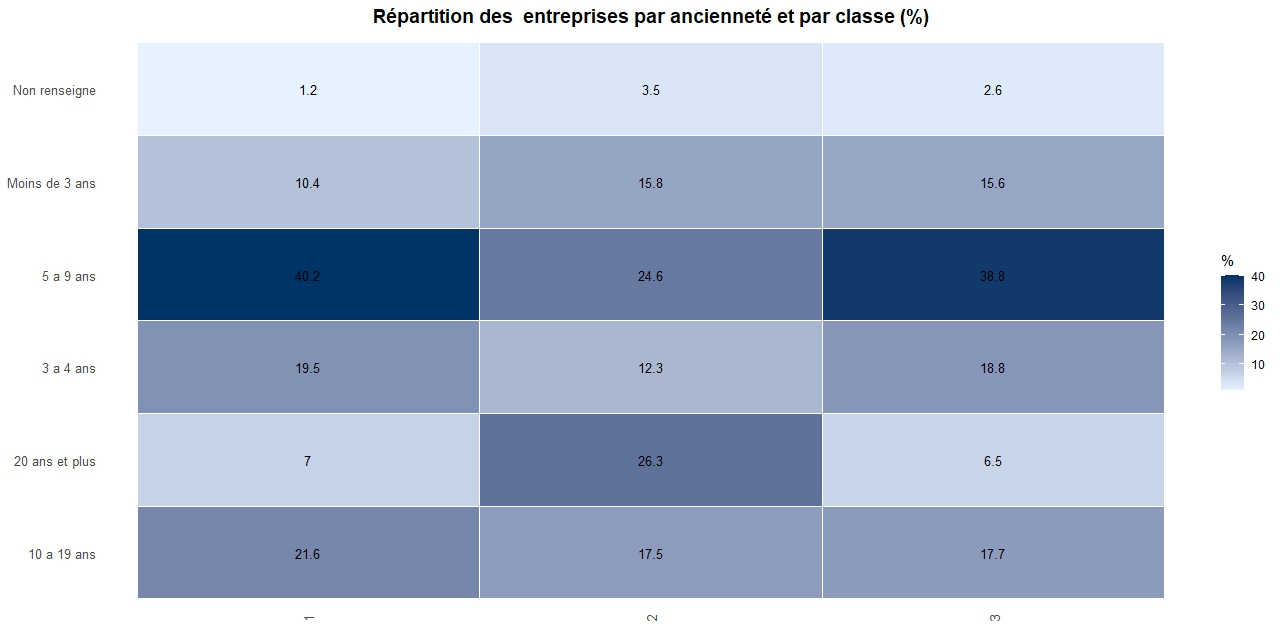
\includegraphics[width=\textwidth]{classe_et_anciennete.jpeg}
					\caption{Répartition des classes par ancienneté }
					\label{fig:rep_class_anc}
				\end{minipage}
				\hfill
				\begin{minipage}{0.48\textwidth}
					\centering
					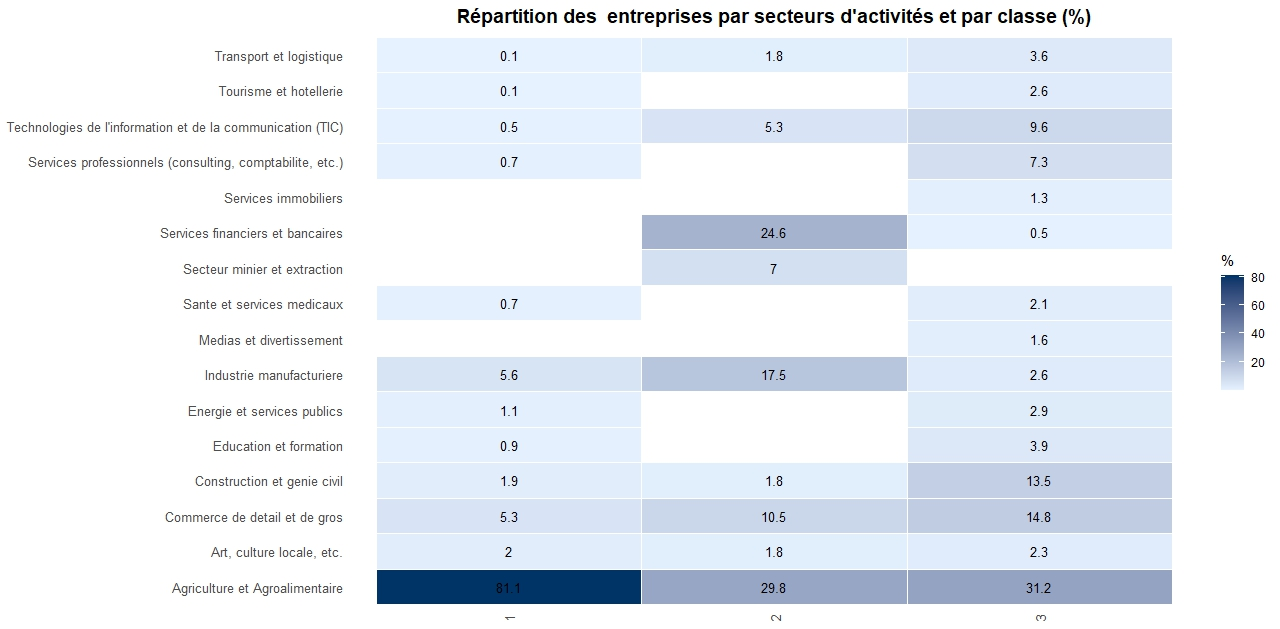
\includegraphics[width=\textwidth]{classes_et_secteurs_activites.jpeg}
					\caption{Répartition des classes par secteur d'activité}
					\label{fig:rep_classe_secteur}
				\end{minipage}
			\end{figure}
			\begin{figure}[H]
				\centering
				\begin{minipage}{0.48\textwidth}
					\centering
					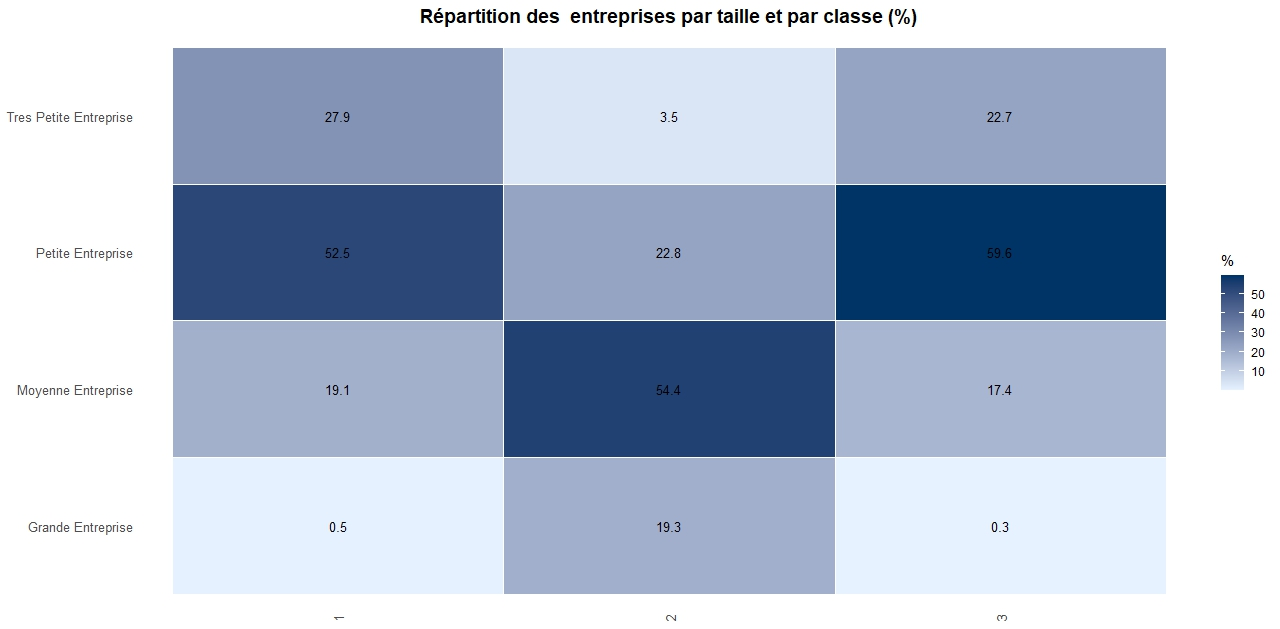
\includegraphics[width=\textwidth]{classes_et_tailles.jpeg}
					\caption{Répartition des classes par taille}
					\label{fig:rep_classe_taille}
				\end{minipage}
				\hfill
				\begin{minipage}{0.48\textwidth}
					\centering
					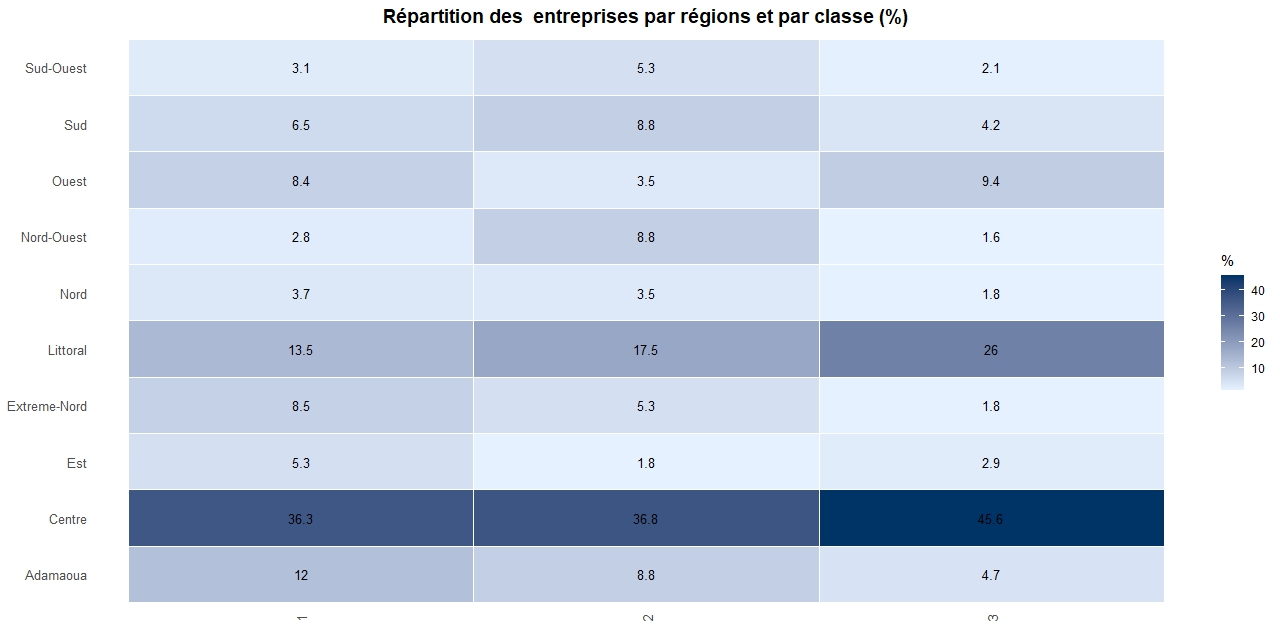
\includegraphics[width=\textwidth]{classes_et_regions.jpeg}
					\caption{Répartition des classes par région}
					\label{fig:rep_classe_region}
				\end{minipage}
			\end{figure}
			
			
			\subsubsection{Analyse Factorielle Discriminante (AFD)}
			
			L'AFD est conduite en aval de la CAH afin de valider la qualité de
			la partition obtenue et d'identifier les variables qui discriminent
			le mieux les trois classes d'entreprises \cite{saporta_2010}. Elle
			permet de répondre à deux questions complémentaires~: les classes
			identifiées sont-elles suffisamment distinctes pour être considérées
			comme des groupes homogènes~? Quelles variables permettent de les
			distinguer le plus efficacement~?
			
			\paragraph{Axes discriminants et pouvoir discriminant}
			
			\begin{figure}[H]
				\centering
				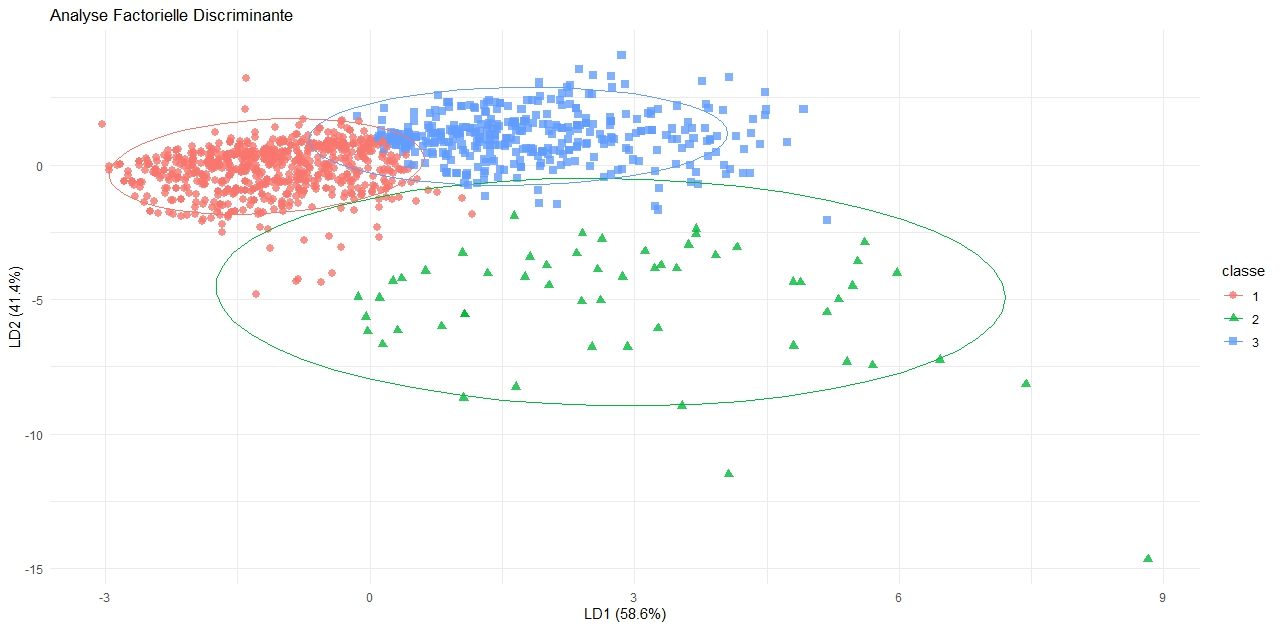
\includegraphics[width=0.85\textwidth]{AFDProjectionDesObservations.jpeg}
				\caption{Projection des entreprises et des centres de classes
					sur les axes discriminants de l'AFD}
				\label{fig:afd_projection}
			\end{figure}
			
			Le graphique de projection des observations met en évidence une excellente séparation globale des trois classes sur le plan formé par les deux premiers axes discriminants, qui captent ensemble 100 \% du pouvoir de séparation (58.6 \% pour LD1 et 41.4 \% pour LD2). Les ellipses de confiance à 95 \% confirment visuellement la pertinence statistique du modèle : bien qu'un léger chevauchement existe entre les classes 1 et 3, les trois nuages de points se structurent de manière distincte sans concentration massive au centre.
			
			
			\paragraph{Les axes factoriels obtenus}

L'Analyse Factorielle Discriminante (AFD) consiste à construire des combinaisons
linéaires des variables initiales --- appelées fonctions discriminantes canoniques ---
de manière à maximiser la variance inter-classes tout en minimisant la variance
intra-classes. Chaque axe obtenu (LD1, LD2, \ldots) représente ainsi une direction
de l'espace factoriel le long de laquelle les groupes issus de la Classification
Ascendante Hiérarchique (CAH) sont séparés de façon optimale. Les coefficients
associés à chaque variable sur ces axes, présentés dans le tableau~\ref{tab:variables_ld},
renseignent sur la contribution relative de chacune d'elles à la discrimination
entre les classes.
		
		\begin{table}[H]
			\centering
			\caption{Coefficients des variables sur les fonctions discriminantes canoniques}
			\label{tab:variables_ld}
			\renewcommand{\arraystretch}{1.4}
			\begin{tabularx}{\textwidth}{>{\raggedright\arraybackslash}X
					>{\centering\arraybackslash}p{3cm}
					>{\centering\arraybackslash}p{3cm}}
				\toprule
				\rowcolor{primary!15}
				\textbf{Variable} & \textbf{LD1} & \textbf{LD2} \\
				\midrule
				
				Dim1
				& 3,4117 & 0,8420 \\
				
				\rowcolor{lightgray}
				Dim2
				& 0,5020 & $-$2,8215 \\
				
				Dim3
				& 1,0018 & $-$2,3454 \\
				
				\rowcolor{lightgray}
				Dim4
				& 0,7551 & $-$2,1043 \\
				
				Dim5
				& $-$0,5523 & 1,0850 \\
				
				\bottomrule
			\end{tabularx}
		\end{table}
		
		
		
		% --- Commentaires analytiques (à intégrer dans le texte du mémoire) ---
		%
		 Le tableau~\ref{tab:variables_ld} présente les coefficients standardisés des variables
		 sur les deux premières fonctions discriminantes canoniques (LD1 et LD2).
		
		 \paragraph{Fonction LD1 — Axe de discrimination principal}
		 La première fonction discriminante est dominée par \textbf{Dim1} (coefficient = 3,41),
		 qui exerce la contribution la plus élevée en valeur absolue parmi toutes les variables.
		 Les variables Dim3 (1,00) et Dim4 (0,76) contribuent également positivement à LD1,
		 tandis que Dim5 présente une contribution négative modérée (--0,55). Dim2 (0,50) joue
		 un rôle secondaire sur cet axe. LD1 semble donc principalement structuré autour de
		 Dim1, qui peut être interprétée comme la dimension discriminante la plus puissante
		 entre les groupes.
		
		 \paragraph{Fonction LD2 — Axe secondaire de séparation}
		 La seconde fonction discriminante oppose fortement Dim2 (--2,82), Dim3 (--2,35)
		 et Dim4 (--2,10) aux variables Dim1 (0,84) et Dim5 (1,09), toutes deux à contribution
		 positive. LD2 capte ainsi une structure de variation orthogonale à LD1, permettant
		 d'affiner la séparation entre les groupes que LD1 ne distingue pas suffisamment.\\
		 
		 
		
		
		% ============================================================
		%  TABLEAU 2 — Indicateurs de performance du modèle
		% ============================================================
		
		
		Au-delà de la représentation factorielle, l'AFD poursuit un objectif de classification
		prédictive. À partir des fonctions discriminantes estimées, chaque observation est
		affectée à la classe dont le centroïde lui est le plus proche au sens de la distance
		de Mahalanobis, ce qui tient compte des corrélations entre variables et de la
		dispersion propre à chaque groupe. Les performances de ce modèle de classification
		sont évaluées à l'aide d'une matrice de confusion établie sur les données de test,
		dont les principaux indicateurs --- précision globale, indice Kappa de Cohen et
		tests de significativité --- sont consignés dans le tableau~\ref{tab:scores_modele}.
		\begin{table}[H]
			\centering
			\caption{Indicateurs de performance du modèle discriminant}
			\label{tab:scores_modele}
			\renewcommand{\arraystretch}{1.4}
			\begin{tabularx}{\textwidth}{>{\raggedright\arraybackslash}X
					>{\centering\arraybackslash}p{3.5cm}
					>{\centering\arraybackslash}p{3cm}}
				\toprule
				\rowcolor{primary!15}
				\textbf{Indicateur} & \textbf{Valeur} & \textbf{Interprétation} \\
				\midrule
				
				Accuracy
				& 0,9724 & Excellent \\
				
				\rowcolor{lightgray}
				Kappa de Cohen
				& 0,9435 & Accord quasi-parfait \\
				
				Accuracy Lower (IC 95\,\%)
				& 0,9614 & — \\
				
				\rowcolor{lightgray}
				Accuracy Upper (IC 95\,\%)
				& 0,9809 & — \\
				
				Accuracy Null
				& 0,6307 & Seuil classifieur naïf \\
				
				\rowcolor{lightgray}
				Accuracy P-value
				& $5{,}16 \times 10^{-183}$ & Hautement significatif \\
				
				McNemar P-value
				& $8{,}50 \times 10^{-7}$ & Significatif ($p < 0{,}05$) \\
				
				\bottomrule
			\end{tabularx}
		\end{table}
		
		% --- Commentaires analytiques (à intégrer dans le texte du mémoire) ---
		%
		 Le tableau~\ref{tab:scores_modele} synthétise les métriques d'évaluation du modèle
		 discriminant appliqué aux données de l'étude.
		
		 \paragraph{Précision globale (Accuracy)}
		 Le modèle affiche une précision globale de \textbf{97,24\,\%}, ce qui traduit un très
		 haut niveau de classification correcte des observations. L'intervalle de confiance à
		 95\,\% est étroit [96,14\,\% -- 98,09\,\%], confirmant la stabilité de cette estimation.
		
		 \paragraph{Indice Kappa de Cohen}
		 Le coefficient Kappa vaut \textbf{0,9435}, ce qui correspond à un accord quasi-parfait
		 entre les classes prédites et les classes réelles (seuil conventionnel : Kappa $> 0{,}80$
		 = très bon accord). Cet indicateur est particulièrement pertinent en présence de classes
		 déséquilibrées, car il corrige la précision en tenant compte du hasard.
		
		 \paragraph{Comparaison au classifieur naïf}
		 L'\textit{Accuracy Null} de 63,07\,\% représente la performance d'un classifieur trivial
		 attribuant systématiquement la classe majoritaire. Le gain de performance du modèle
		 par rapport à ce seuil est de $+34{,}17$ points de pourcentage, ce qui illustre
		 l'apport réel du modèle discriminant.
		
		 \paragraph{Significativité statistique}
		 La p-valeur associée à l'accuracy ($5{,}16 \times 10^{-183}$) est extrêmement faible,
		 rejetant sans ambiguïté l'hypothèse nulle selon laquelle le modèle ne serait pas meilleur
		 qu'un classifieur aléatoire. De même, le test de McNemar (p = $8{,}50 \times 10^{-7}$)
		 indique une asymétrie significative dans la matrice de confusion, suggérant que les
		 erreurs du modèle ne sont pas distribuées de façon uniforme entre les classes.
		
	
%=============================================================
\section{Présentation de la plateforme \textit{Business Partnership}}
\label{sec:presentation_plateforme}
%=============================================================

La présente section est consacrée à la présentation de la plateforme
\textit{Business Partnership}, fruit de l'ensemble des travaux de
conception et de développement décrits dans les chapitres précédents. Cette présentation
s'appuie sur des captures d'écran de la plateforme dans son état
fonctionnel actuel, accompagnées de descriptions techniques précises
permettant d'apprécier la cohérence entre les exigences formulées
dans le cahier des charges et les réalisations effectives.

%-------------------------------------------------------------
\subsection{Architecture générale de la plateforme}
\label{subsec:architecture_generale}
%-------------------------------------------------------------

La plateforme \textit{Business Partnership} est une application web
développée selon le paradigme \textbf{MVT (Modèle-Vue-Template)}
proposé par le framework Django. Son architecture repose sur une
séparation claire entre trois couches fonctionnelles~: la couche
de présentation, qui assure le rendu des interfaces utilisateur via
les templates HTML et CSS~; la couche métier, qui contient la logique
applicative;
et la couche de données, qui assure la persistance et la restitution
structurée des informations via l'ORM de Django et la base de données
SQLite.

%-------------------------------------------------------------
\subsection{Interface utilisateur}
\label{subsec:interface_utilisateur}
%-------------------------------------------------------------

L'interface utilisateur de la plateforme \textit{Business Partnership}
a été conçue dans l'optique d'offrir une expérience de navigation intuitive, cohérente
et accessible. L'ensemble des
composants visuels repose sur le framework CSS \textbf{Bootstrap},
qui garantit une cohérence graphique entre les différentes pages
de la plateforme et une adaptation automatique de l'interface
aux différentes tailles d'écran (\textit{responsive design}).

\subsubsection{Page de login}

La page login permet à l'utilisateur de se connecter à son compte si ce dernier existe déjà. Cette page donne également la possibilité de créer un compte avec ses informations. La validation de son compte sera fait par l'administrateur du site après examen des documents.
\begin{figure}[H]
	\centering
	
\includegraphics[width=\textwidth]{login.png}
	\caption{Page de login
		\textit{Business Partnership}}
	\label{fig:screen_accueil}
\end{figure}

\subsubsection{Page de création de compte}

La page de création de compte demande des informations basiques sur l'entreprise et trois documents dont un facultatif.

\begin{figure}[H]
	\centering
	
\includegraphics[width=\textwidth]{creationDeCompte.png}
	\caption{Page de création de compte}
	\label{fig:creationDeCompte}
\end{figure}
\subsubsection{Validation de compte par l'administrateur}
L'administrateur du site recoit la demande d'adhésion et la valide ou l'invalide.
\begin{figure}[H]
	\centering
	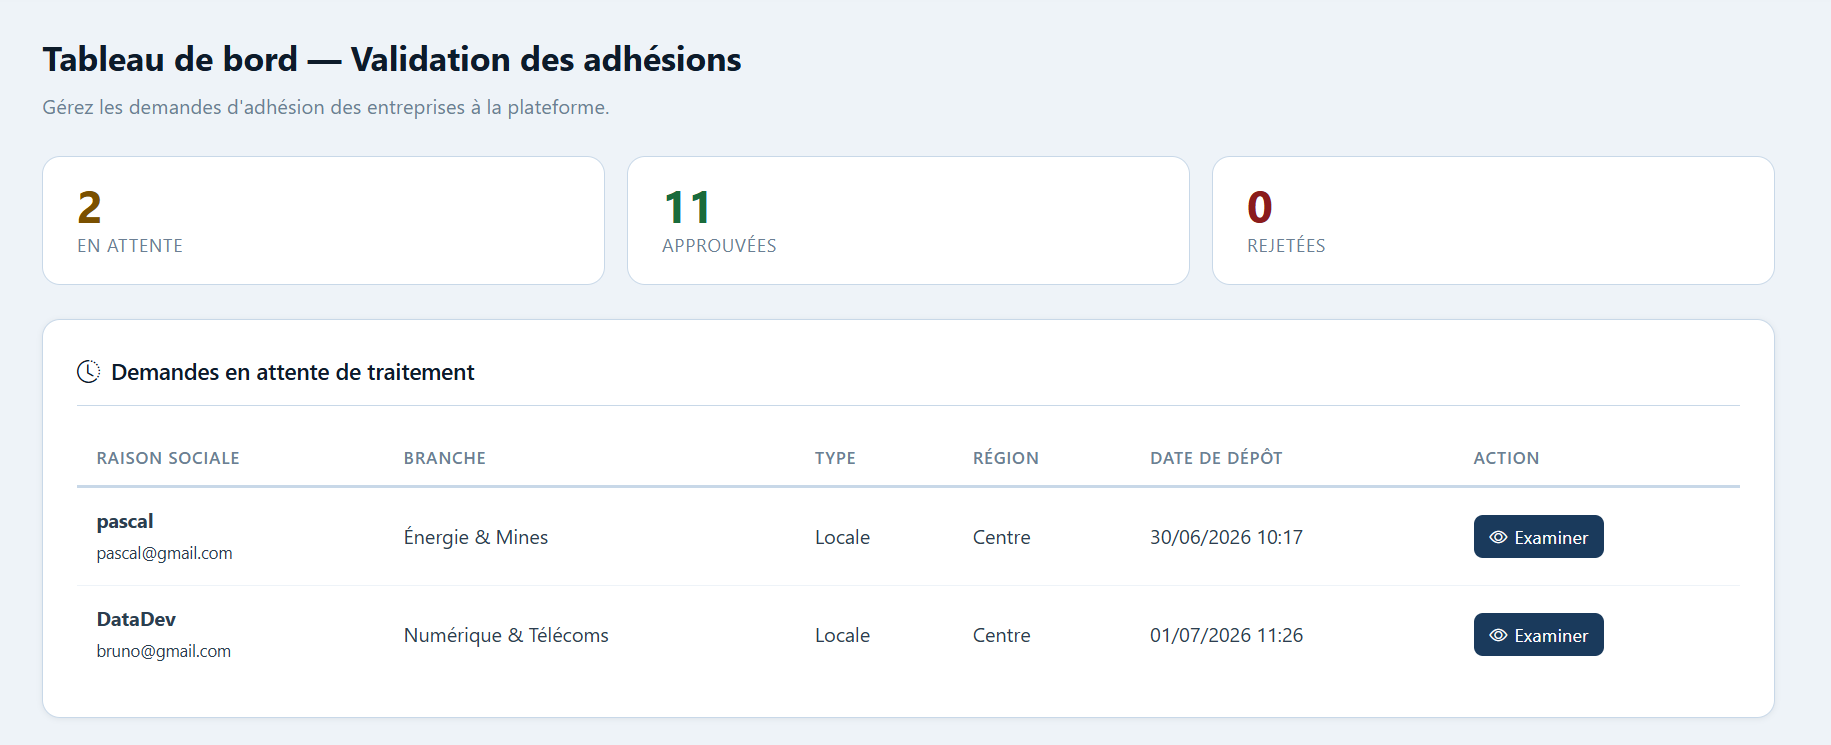
\includegraphics[width=\textwidth]{demande.png}
	\caption{Les demandes}
	\label{fig:demande}
\end{figure}
\begin{figure}[H]
	\centering
	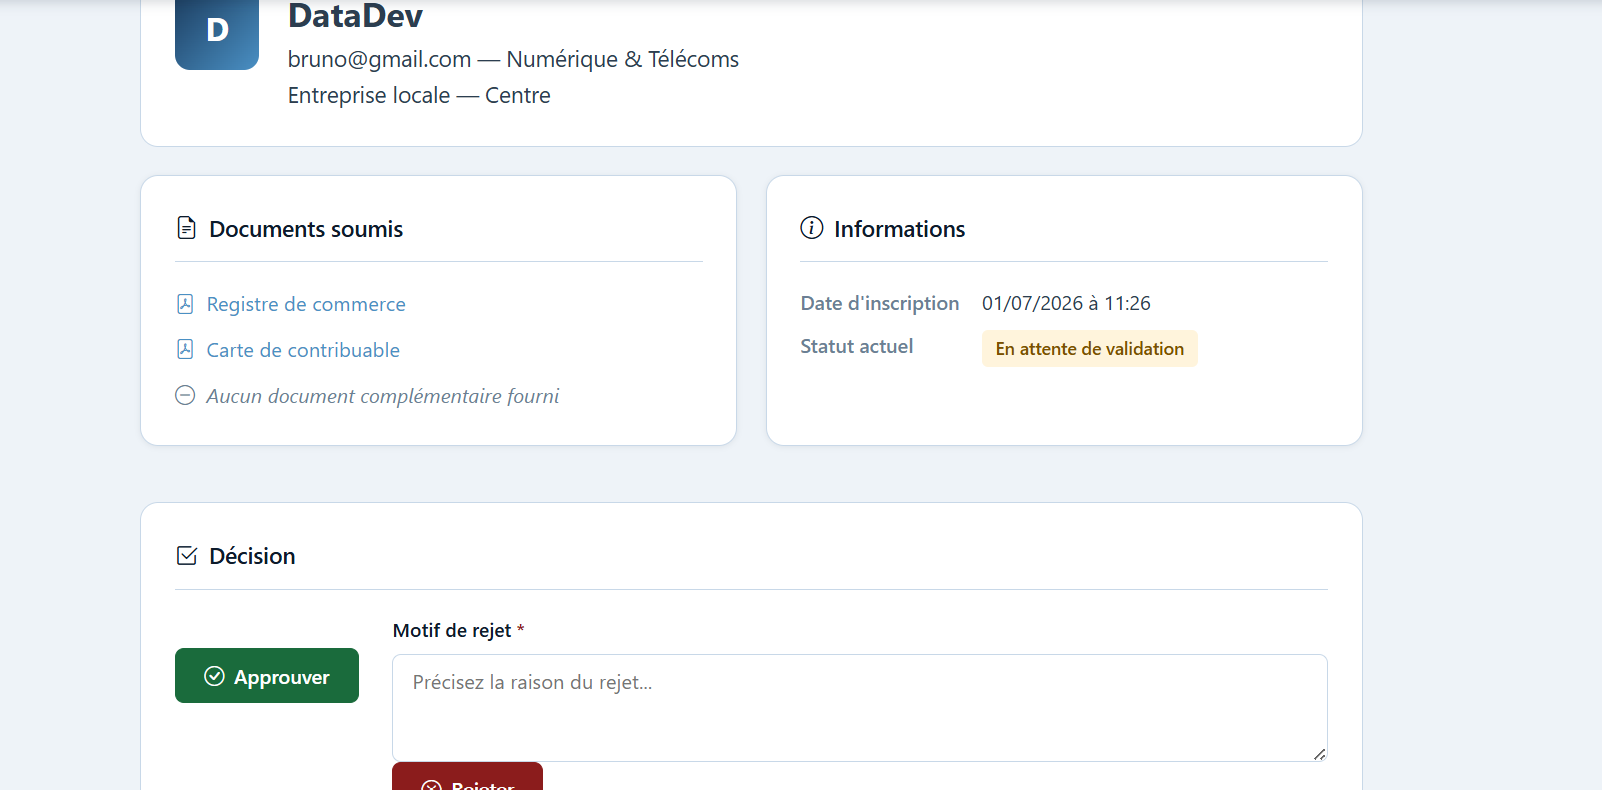
\includegraphics[width=\textwidth]{validation.png}
	\caption{Validation de compte}
	\label{fig:validation}
\end{figure}
\subsubsection{Tableau de bord de l'entreprise}
Le tableau de bord de l'entreprise permet de définir ses besoins, ses offres, de modifier ses informations et de visualiser les entreprises recommandées.

\begin{figure}[H]
	\centering
	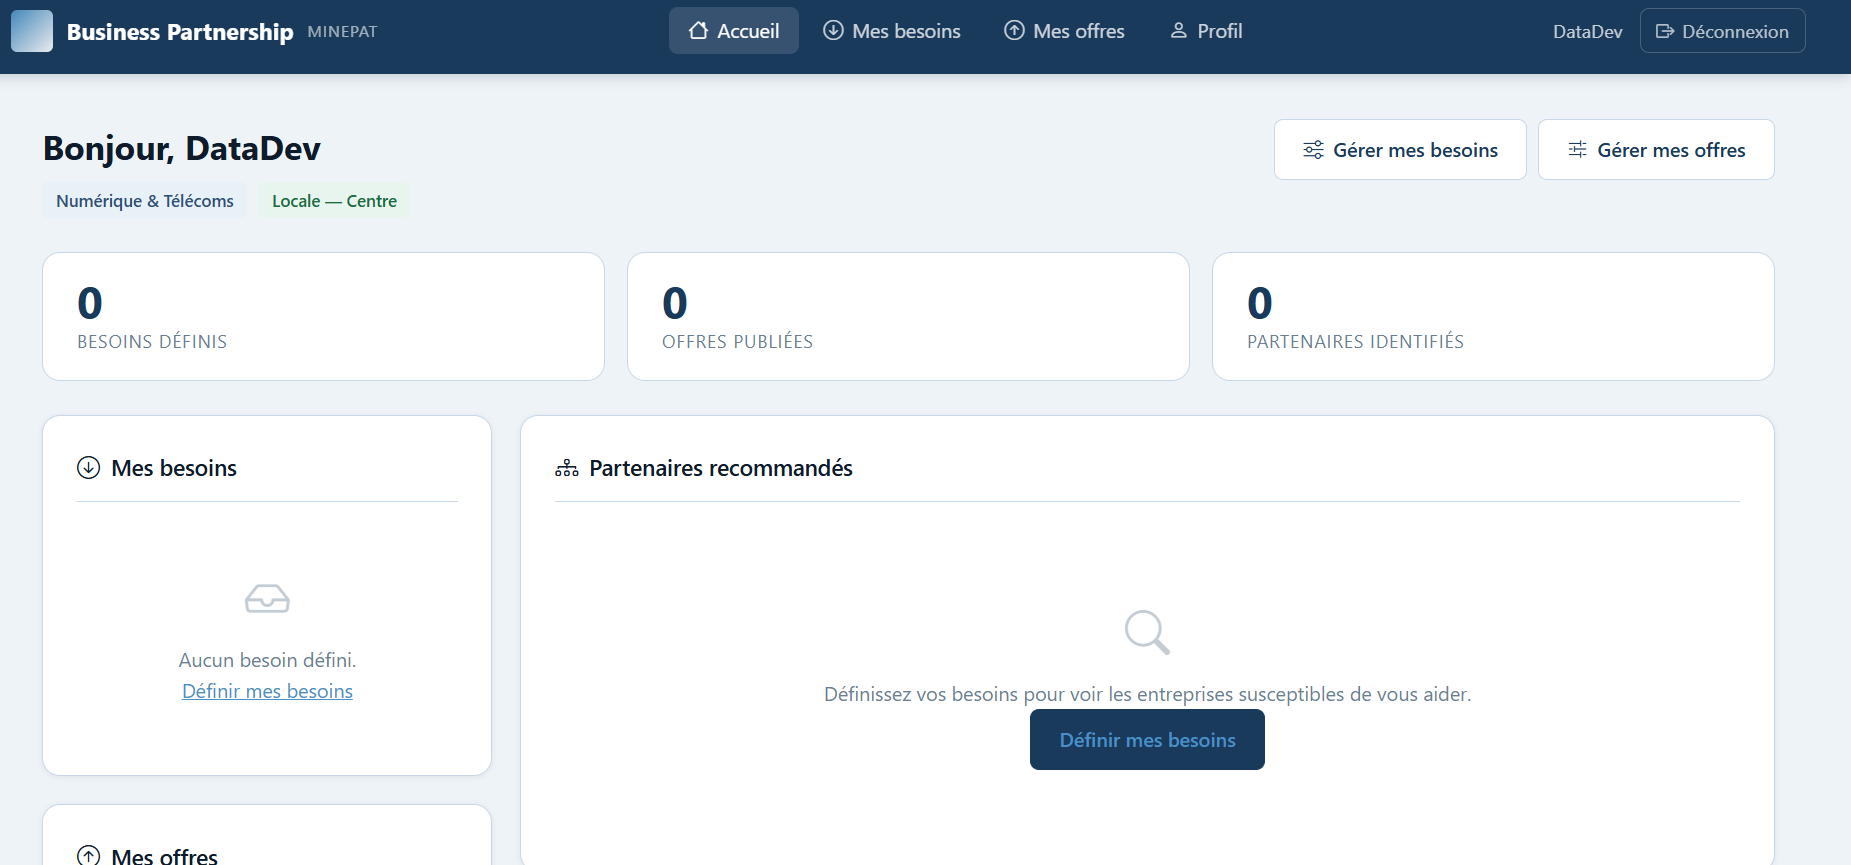
\includegraphics[width=\textwidth]{tableauDeBordEntreprise.png}
	\caption{Tableau de bord de l'entreprise}
	\label{fig:tableauDeBord}
\end{figure}

\subsubsection{Tableau de bord administrateur}

Le tableau de bord administrateur offre aux agents du \gls{minepat}
une vision panoramique et en temps réel de l'activité de la
plateforme. Une section dédiée à la
gestion des demandes d'inscription en attente de validation permet
à l'administrateur de consulter, approuver ou rejeter chaque
demande après vérification des informations fournies. 

\begin{figure}[H]
	\centering
	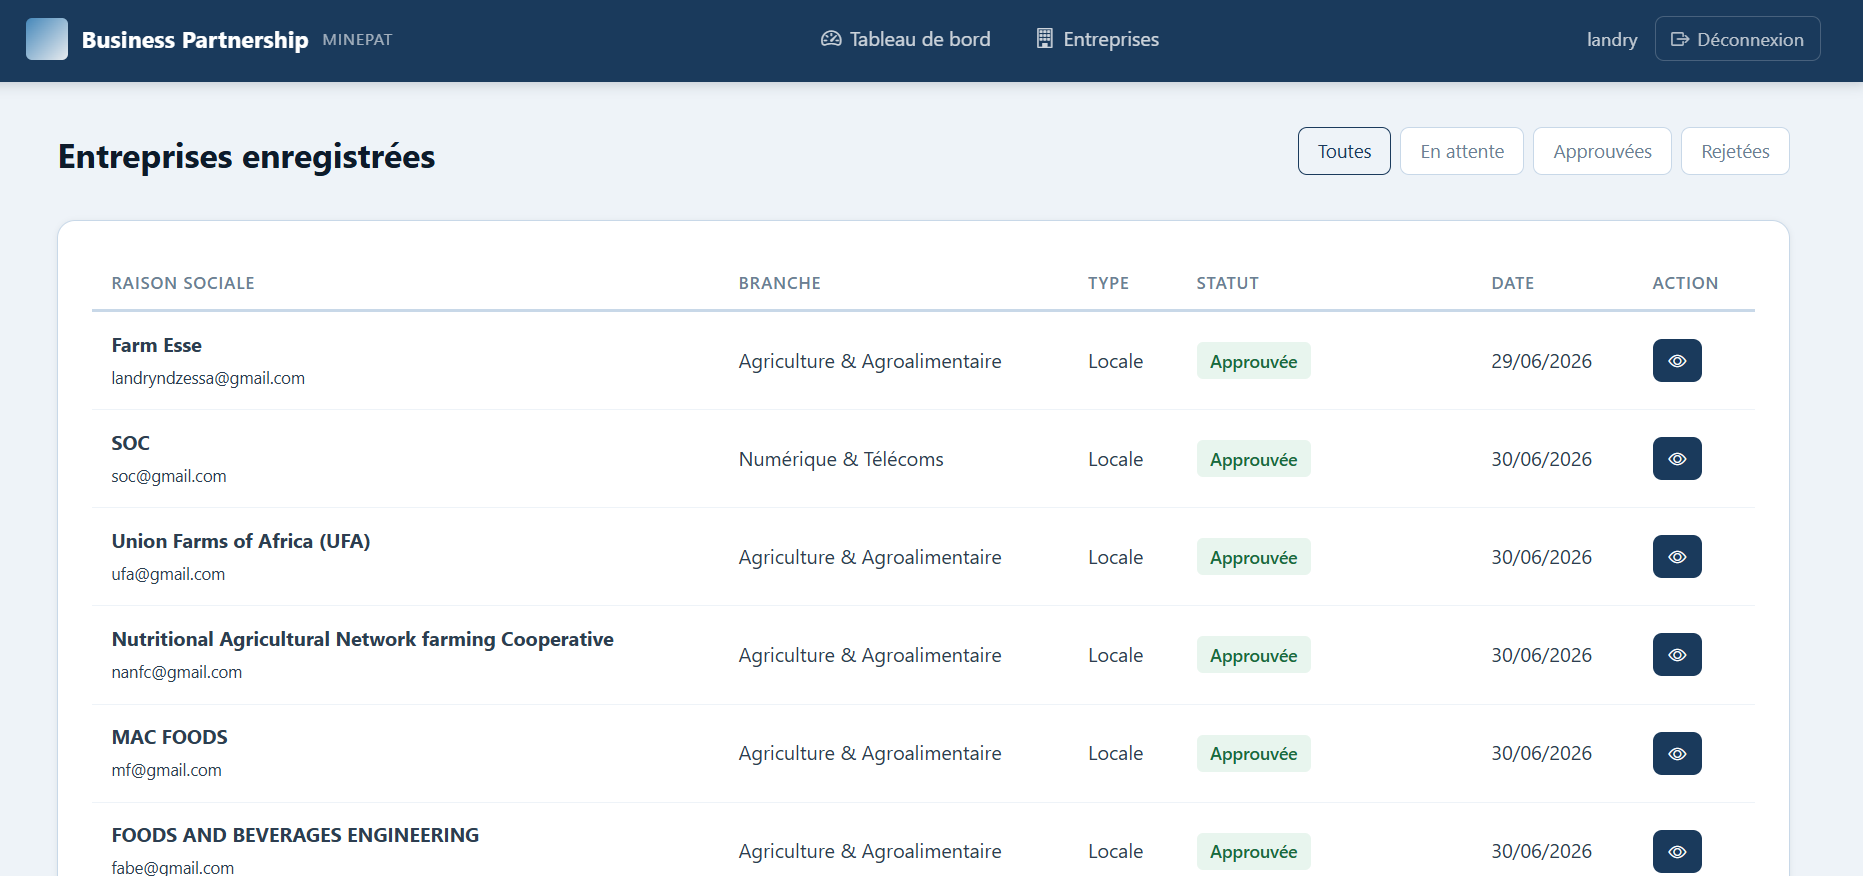
\includegraphics[width=\textwidth]{tableauDeBordAdmin.png}
	\caption{Tableau de bord de l'espace administrateur}
	\label{fig:admin}
\end{figure}


\subsubsection{Requ\^ete pour la mise en relation}

La mise en relation des entreprises est basée sur l'offre et la demande. Le classement est fait par ordre décroissant des entreprises les plus compatibles avec les besoins de l'entreprise. C'est à dire les entreprises offrant des serices dont vous avez le plus besoin.

\begin{figure}[H]
	\centering
	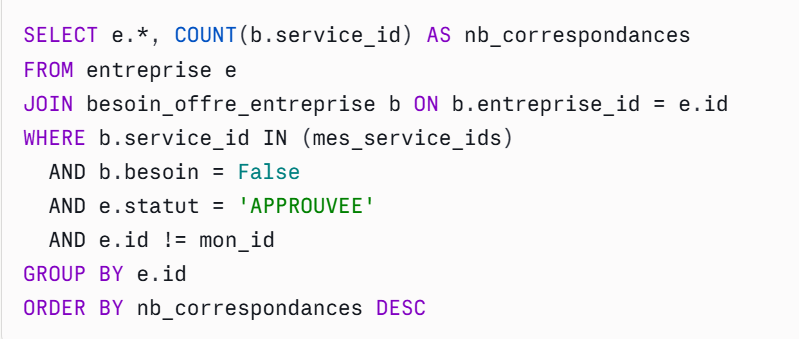
\includegraphics[width=\textwidth]{requeteSQL.png}
	\caption{Requ\^ete pour la mise en relation }
	\label{fig:admin}
\end{figure}

	\subsection{Perspectives}
	
L'onjectif principal de le plateforme numérique developpée dans le cadre de ce travail est de proposer un environnement de collaboration entre les entreprises basé sur les offres et les besoins de ceux-ci. Les évolutions potentielles envisagées pourraient consister à:
\begin{itemize}
	\item Donner la possibilité aux entreprises d'exposer leurs produits visible par les autres. La plateforme pourra donc s'étendre à une vitrine non seuelement de mise en relation mais aussi d'exposition des produits des entreprises;
	\item Intégrer un système de communication direct entre les entreprises sur la plateforme pour faciliter les échanges;
	\item Construire un outil d'aide à la décision pour accompagner les entreprises sur la base des données receuillies.
\end{itemize}

\section{Tests de l'application}

\subsection{Stratégie de test}
Les tests ont été réalisés avec le framework de tests intégré à Django,
qui repose sur \texttt{unittest} de la bibliothèque standard Python.
Chaque test s'exécute dans une base de données isolée en mémoire,
recréée et détruite automatiquement à chaque exécution, garantissant
l'indépendance des résultats.

\subsection{Couverture fonctionnelle}
Cinquante-six (56) cas de test ont été définis, répartis en huit groupes
couvrant l'ensemble des fonctionnalités de la plateforme
(tableau~\ref{tab:tests}).

\begin{table}[htbp]
	\centering
	\caption{Récapitulatif des tests par groupe}
	\label{tab:tests}
	\begin{tabular}{clc}
		\hline
		\textbf{Groupe} & \textbf{Fonctionnalités couvertes} & \textbf{Tests} \\
		\hline
		T1 & Modèles et intégrité des données     & 8  \\
		T2 & Authentification et contrôle d'accès & 7  \\
		T3 & Inscription des entreprises           & 6  \\
		T4 & Validation par le ministère           & 6  \\
		T5 & Gestion des besoins et offres         & 8  \\
		T6 & Algorithme de mise en relation        & 7  \\
		T7 & API JSON                              & 5  \\
		T8 & Isolation et sécurité des données     & 7  \\
		\hline
		\textbf{Total} & & \textbf{56} \\
		\hline
	\end{tabular}
\end{table}

\subsection{Faits saillants}
Parmi les comportements validés, on retiendra notamment~:
\begin{itemize}
	\item le blocage de la connexion pour toute entreprise dont le dossier
	n'a pas encore été approuvé par le ministère~;
	\item le classement décroissant des partenaires par nombre de
	correspondances, tel que spécifié dans le cahier des charges~;
	\item la protection contre l'accès croisé aux données~: une entreprise
	ne peut pas modifier ou supprimer les enregistrements
	appartenant à une autre~;
	\item la protection CSRF active sur tous les formulaires POST~;
	\item la contrainte d'unicité sur la table de faits qui empêche
	les doublons besoins/offres.
\end{itemize}
\section*{Conclusion}
La cartographie des besoins des entreprises, réalisée à l'aide d'outils tant théoriques que pratiques, a permis de mettre en évidence trois catégories distinctes. L'identification du profil des entreprises et des besoins les plus récurrents au sein de chaque classe pourrait ainsi guider les pouvoirs publics dans la mise en œuvre d'actions ciblées. Ces derniers n'étant pas en mesure de répondre à l'ensemble des sollicitations multiformes des entreprises, la plateforme numérique développée dans le cadre de ce travail vient non seulement accompagner ces structures, mais aussi appuyer les interventions du \gls{minepat}. 
	%============================================================
	%  CONCLUSION GÉNÉRALE
	%============================================================
	\chapter*{Conclusion Générale}
	\addcontentsline{toc}{chapter}{Conclusion Générale}
	\markboth{Conclusion Générale}{Conclusion Générale}
	
L'atteinte des objectifs de la Stratégie Nationale de Développement 2020-2030 (\gls{snd30}) constitue l'une des préoccupations majeures du gouvernement camerounais. Dans cette perspective, le secteur privé a été identifié comme le principal moteur de la croissance économique, rendant indispensable l'amélioration continue du climat des affaires pour stimuler sa compétitivité. Le présent travail s'est inscrit dans cette dynamique à travers l'exploitation des données de l'enquête nationale initiée par le \gls{minepat}.

Le volet analytique de cette étude a mis en évidence les caractéristiques structurelles du tissu entrepreneurial national, révélant notamment une économie encore faiblement orientée vers la transformation industrielle et souffrant d'un déficit de valeur ajoutée. L'application des méthodes d'analyse statistique multidimensionnelle a toutefois permis de segmenter les entreprises en trois profils distincts, offrant ainsi une grille de lecture factuelle pour orienter les futures interventions publiques. 

Face au constat que l'État ne peut répondre seul aux besoins multiformes de ces acteurs, la plateforme numérique «~Business Partnership~» a été développée comme un outil d'accompagnement direct. En s'appuyant sur une modélisation dimensionnelle adaptée, cette application facilite la mise en relation et la recherche d'opportunités d'affaires entre les entreprises, contribuant ainsi à dynamiser le secteur privé.

En guise d'ouverture, ce travail pose les bases d'un système d'aide à la décision qui pourrait être enrichi à l'avenir. Une perspective intéressante consisterait à intégrer des modules d'analyse prédictive ou d'intelligence artificielle pour recommander automatiquement des partenariats en fonction de l'évolution des besoins des entreprises, consolidant ainsi le rôle de la plateforme comme levier du développement économique national.
	

	%============================================================
	%  BIBLIOGRAPHIE
	%============================================================
	%\printbibliography[heading=bibintoc, title={Bibliographie}]
\newpage
\bibliographystyle{plainnat}
\bibliography{references} % Indiquez le nom de votre fichier .bib sans l'extension
%\printbibliography[title={Bibliographie}] % Génère la liste des références
	%============================================================
	%  ANNEXES
	%============================================================
	
	\chapter*{Questionnaire de l'enquête MINEPAT 2025}
	\label{ann:questionnaire}
	
	\begin{figure}[H]
		\centering
		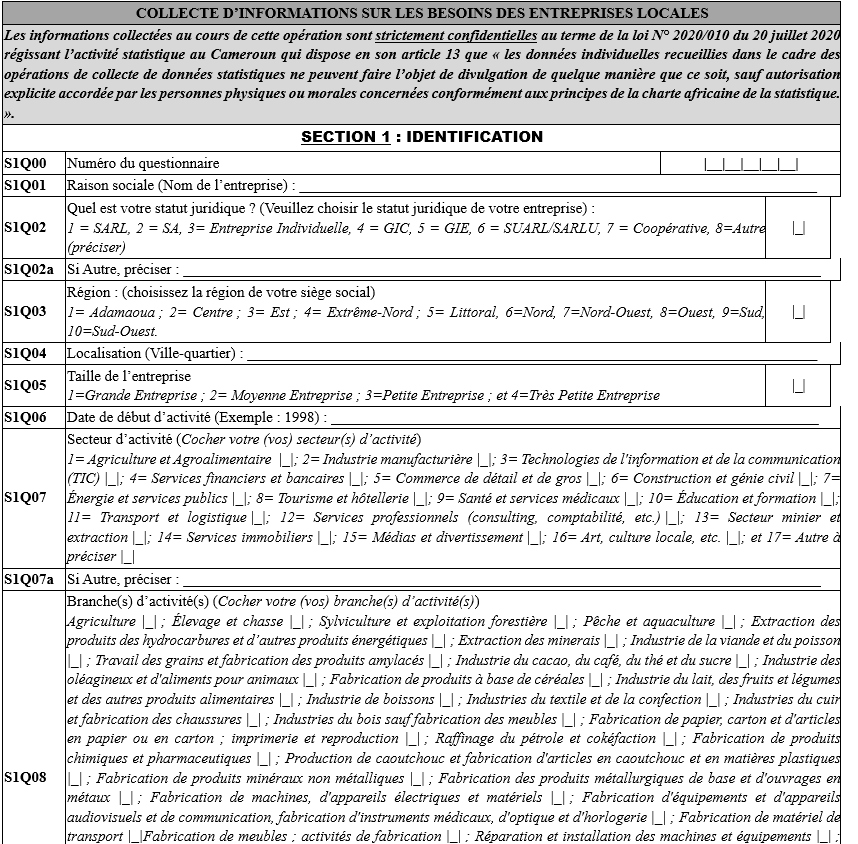
\includegraphics[width=\textwidth]{annexe1.png}
		\caption[Questionnaire 1/3]{Questionnaire 1/3 \footnotemark}
		\label{fig:questionnaire_1}
	\end{figure}
	\footnotetext{Source : Rapport sur l'enquete des besoins des entreprises locales}
	
	\begin{figure}[H]
		\centering
		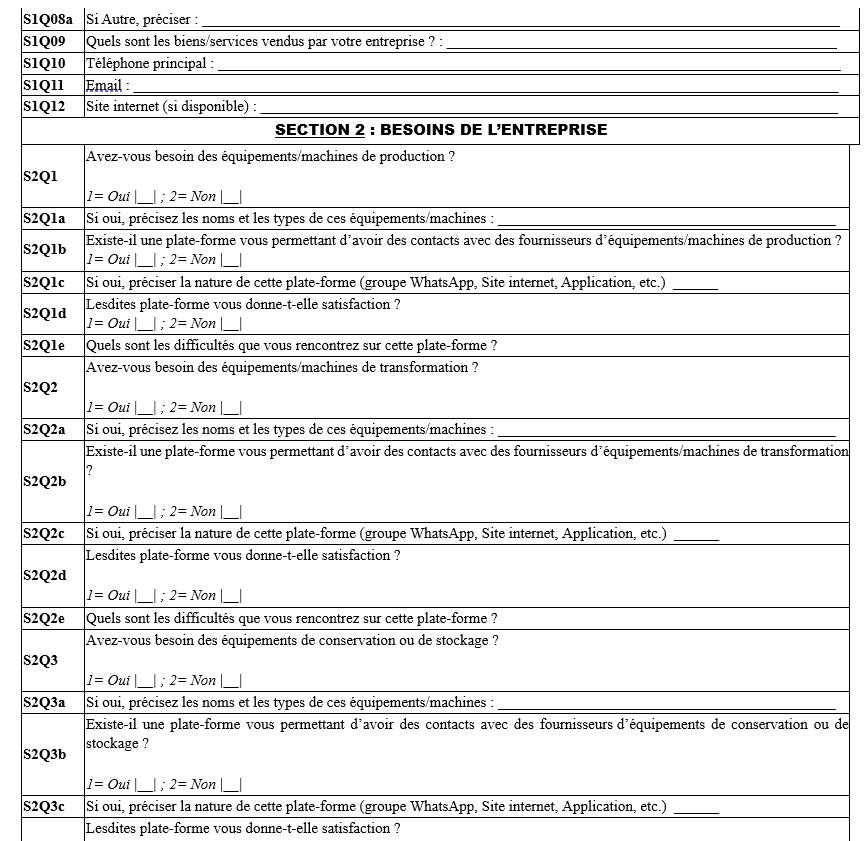
\includegraphics[width=\textwidth]{annexe2.png}
		\caption[Questionnaire 2/3]{Questionnaire 2/3 \footnotemark}
		\label{fig:questionnaire_2}
	\end{figure}
	\footnotetext{Source : Rapport sur l'enquete des besoins des entreprises locales}
	
	\begin{figure}[H]
		\centering
		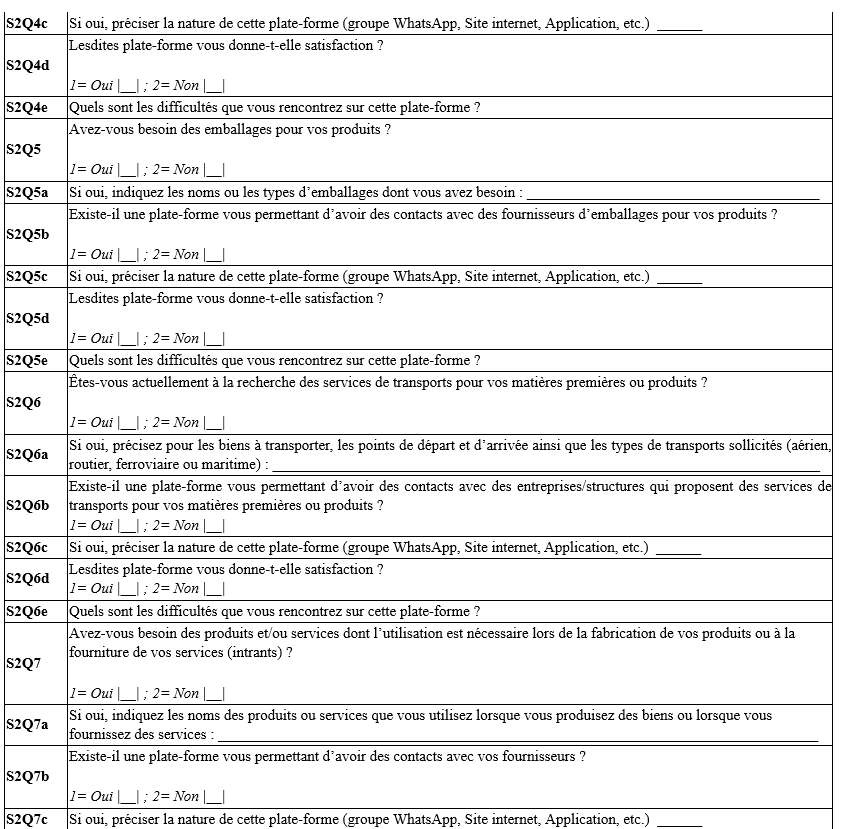
\includegraphics[width=\textwidth]{annexe3.png}
		\caption[Questionnaire 3/3]{Questionnaire 3/3 \footnotemark}
		\label{fig:questionnaire_3}
	\end{figure}
	\footnotetext{Source : Rapport sur l'enquete des besoins des entreprises locales}
	
	
	\chapter*{Publication de l'annonce}
	\label{ann:modele}
	
	\begin{figure}[H]
		\centering
		
\includegraphics[width=\textwidth]{annexe5.jpg}
		\caption[Communiqué d'intérêt public]{Communiqué d'inter\^et public \footnotemark}
		\label{fig:communique}
	\end{figure}
	\footnotetext{Source : Rapport sur l'enquete des besoins des entreprises locales}
	
	\begin{figure}[H]
		\centering
		
\includegraphics[width=\textwidth]{annexe6.jpg}
		\caption[Demande de communiqué à Cameroun Tribune]{Demande de communiqué à cameroun tribune \footnotemark}
		\label{fig:demande_tribune}
	\end{figure}
	\footnotetext{Source : Rapport sur l'enquete des besoins des entreprises locales}
	
	
\end{document}